%%%%%%%%%%%%%%%%%%%%%%%%%%%%%%%%%%%%%%%%%
% Beamer Presentation
% LaTeX Template
% Version 1.0 (10/11/12)
%
% This template has been downloaded from:
% http://www.LaTeXTemplates.com
%
% License:
% CC BY-NC-SA 3.0 (http://creativecommons.org/licenses/by-nc-sa/3.0/)
%
%%%%%%%%%%%%%%%%%%%%%%%%%%%%%%%%%%%%%%%%%

%----------------------------------------------------------------------------------------
%	PACKAGES AND THEMES
%----------------------------------------------------------------------------------------

\documentclass{beamer}

\mode<presentation> {

% The Beamer class comes with a number of default slide themes
% which change the colors and layouts of slides. Below this is a list
% of all the themes, uncomment each in turn to see what they look like.

\usetheme{default}
%\usetheme{AnnArbor}
%\usetheme{Antibes}
%\usetheme{Bergen}
%\usetheme{Berkeley}
%\usetheme{Berlin}
%\usetheme{Boadilla}
%\usetheme{CambridgeUS}
%\usetheme{Copenhagen}
%\usetheme{Darmstadt}
%\usetheme{Dresden}
%\usetheme{Frankfurt}
%\usetheme{Goettingen}
%\usetheme{Hannover}
%\usetheme{Ilmenau}
%\usetheme{JuanLesPins}
%\usetheme{Luebeck}
%\usetheme{Madrid}
%\usetheme{Malmoe}
%\usetheme{Marburg}
%\usetheme{Montpellier}
%\usetheme{PaloAlto}
%\usetheme{Pittsburgh}
%\usetheme{Rochester}
%\usetheme{Singapore}
%\usetheme{Szeged}
%\usetheme{Warsaw}

% As well as themes, the Beamer class has a number of color themes
% for any slide theme. Uncomment each of these in turn to see how it
% changes the colors of your current slide theme.

%\usecolortheme{albatross}
%\usecolortheme{beaver}
%\usecolortheme{beetle}
%\usecolortheme{crane}
%\usecolortheme{dolphin}
%\usecolortheme{dove}
%\usecolortheme{fly}
%\usecolortheme{lily}
%\usecolortheme{orchid}
%\usecolortheme{rose}
%\usecolortheme{seagull}
%\usecolortheme{seahorse}
%\usecolortheme{whale}
%\usecolortheme{wolverine}

%\setbeamertemplate{footline} % To remove the footer line in all slides uncomment this line
\setbeamertemplate{footline}[page number] % To replace the footer line in all slides with a simple slide count uncomment this line

\setbeamertemplate{navigation symbols}{} % To remove the navigation symbols from the bottom of all slides uncomment this line
}
\newenvironment{changemargin}[2]{%
\begin{list}{}{%
\setlength{\topsep}{0pt}%
\setlength{\leftmargin}{#1}%
\setlength{\rightmargin}{#2}%
\setlength{\listparindent}{\parindent}%
\setlength{\itemindent}{\parindent}%
\setlength{\parsep}{\parskip}%
}%
\item[]}{\end{list}}
%\usepackage[greek,german]{babel}
\usepackage{graphicx} % Allows including images
\usepackage{booktabs} % Allows the use of \toprule, \midrule and \bottomrule in tables
\usepackage{amsmath}
\usepackage{slashed}
\usepackage{color}
\usepackage{rotating}
%----------------------------------------------------------------------------------------
%	TITLE PAGE
%----------------------------------------------------------------------------------------

%\title{Benchmarking reconstruction times} % The short title appears at the bottom of every slide, the full title is only on the title page

%\author{\underline{Author} \and Author} % Your name

%\author{{\bf A.~Pathak}, S.~Banerjee and P.N.~Dang}


%\institute[U. Louisville] % Your institution as it will appear on the bottom of every slide, may be shorthand to save space


%\date{{Upgrade Tracking Meeting}\\\today\\} % Date, can be changed to a custom date

%\pgfdeclareimage[height=.75cm]{biglogo}{/afs/cern.ch/user/s/swaban/public/university-of-louisville-logo}
%\titlegraphic{\pgfuseimage{biglogo}} 

\begin{document}

%\begin{frame}
%\titlepage % Print the title page as the first slide
%\end{frame}
%-------------------------------------------------
\begin{frame}
\frametitle{AthAlgSeq For full Reconstruction in HS06 Second}
\vspace*{0.5cm} 
\begin{table}

{\scalebox{.76}{
\begin{tabular}{|l|c|c|c|c|}\hline\hline
Detector  &         $\langle \mu \rangle$=0        &       $\langle \mu \rangle$=60    &     $\langle \mu \rangle$=140     &  $\langle \mu \rangle$=200    \\ \hline
ITk           &         30.39 $\pm$ 0.60                  &             123.98 $\pm$ 1.77          &           379.70 $\pm$ 5.13            &  563.12 $\pm$ 7.93                   \\ \hline\hline
\end{tabular}
}}
\end{table}
\vspace*{1cm}
\begin{table}

{\scalebox{.76}{
\begin{tabular}{|l|c|c|c|c|}\hline\hline
Detector  &         $\langle \mu \rangle$=20        \\ \hline
Run 2       &         114.61 $\pm$ 1.75                \\ \hline\hline
\end{tabular}
}}
\end{table}
\vspace*{1cm}
\end{frame} 
\end{document}
%------------------------------------------------
\iffalse
\begin{frame}
\frametitle{ collinear mass in $H\to e\tau_{had}$ }
\begin{normalsize}
\begin{center}
SR1 and SR2 (left to right) SR3(Below)
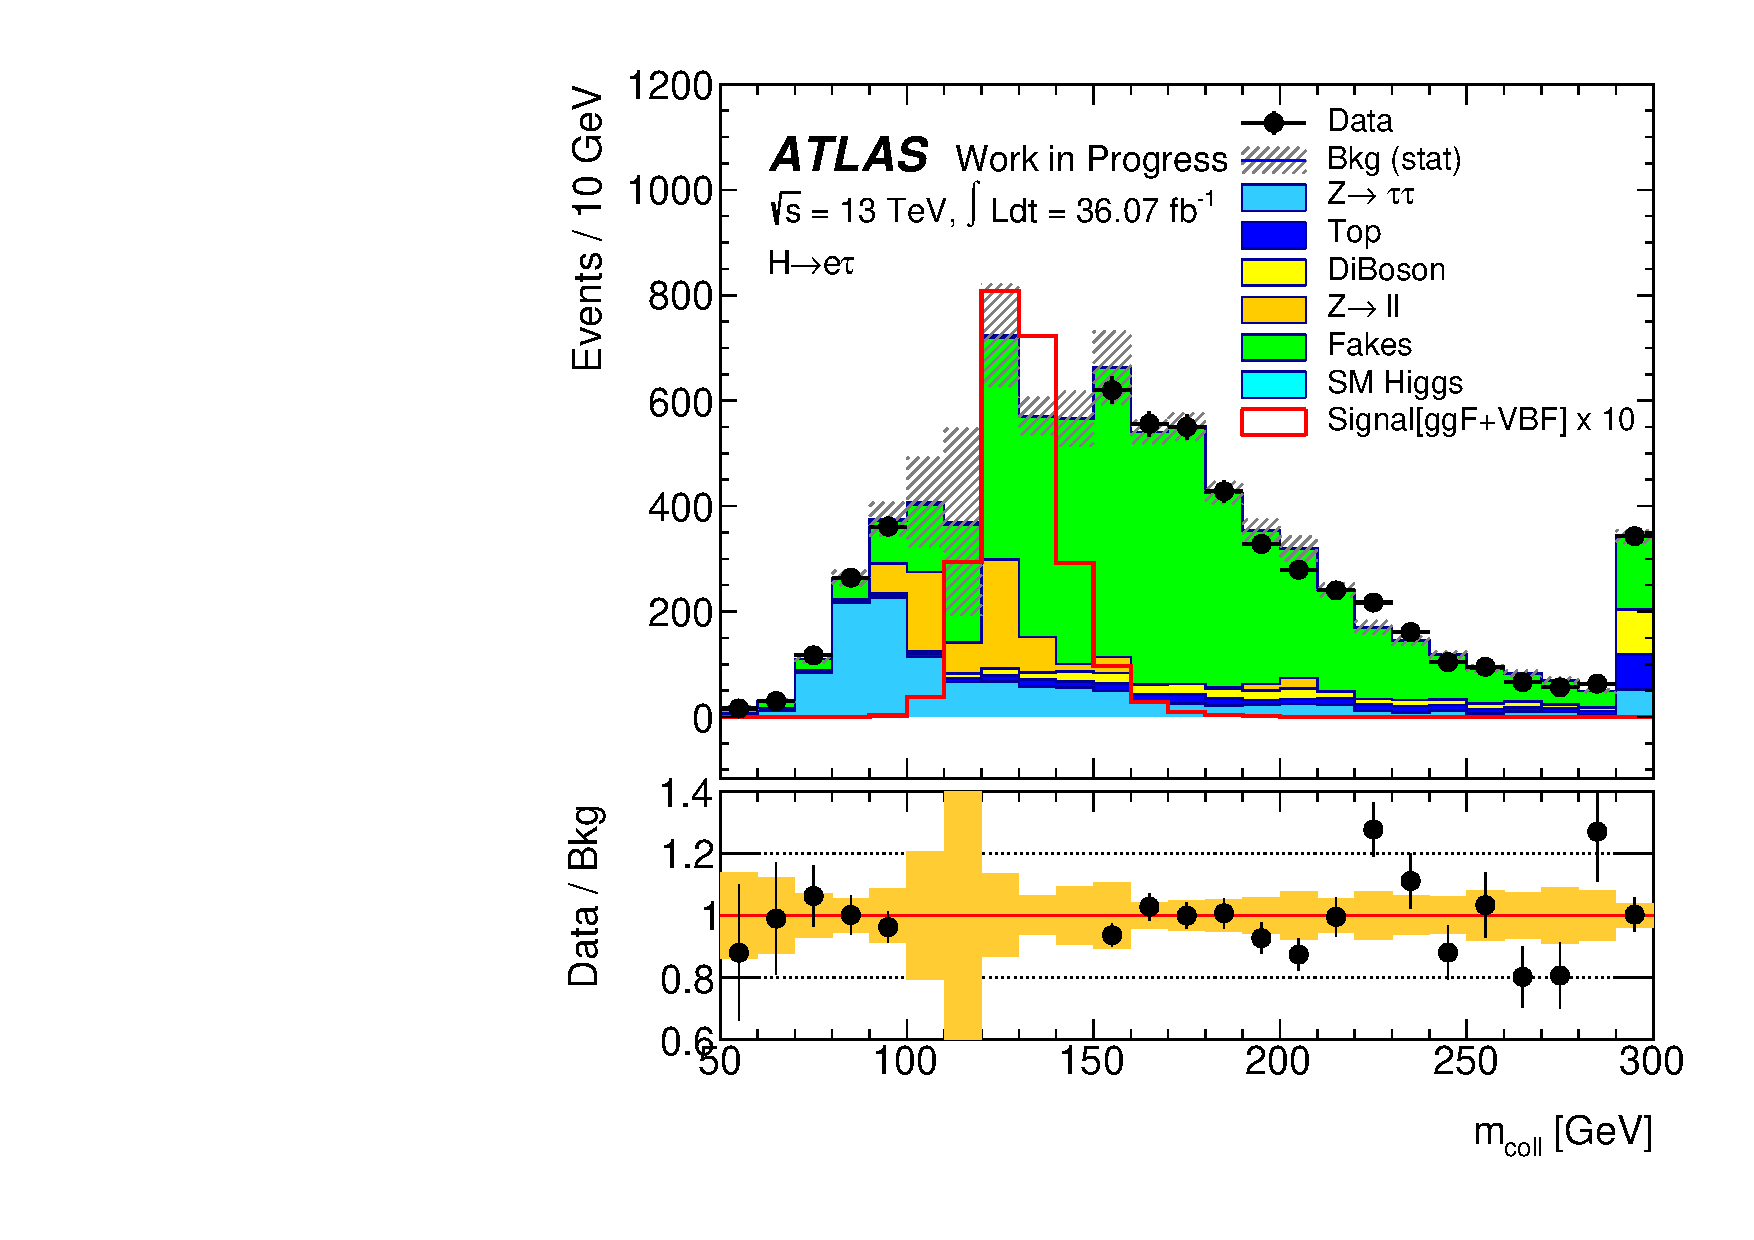
\includegraphics[width=.40\textwidth,height=.40\textheight,type=png,ext=.pdf,read=.pdf]{/afs/cern.ch/user/a/atpathak/afswork/private/xTauFramework/xTauFramework/test_candidacy_20Nov2017/Plots/plots/etau-CutTauMTSR1-collMassBL-lin}
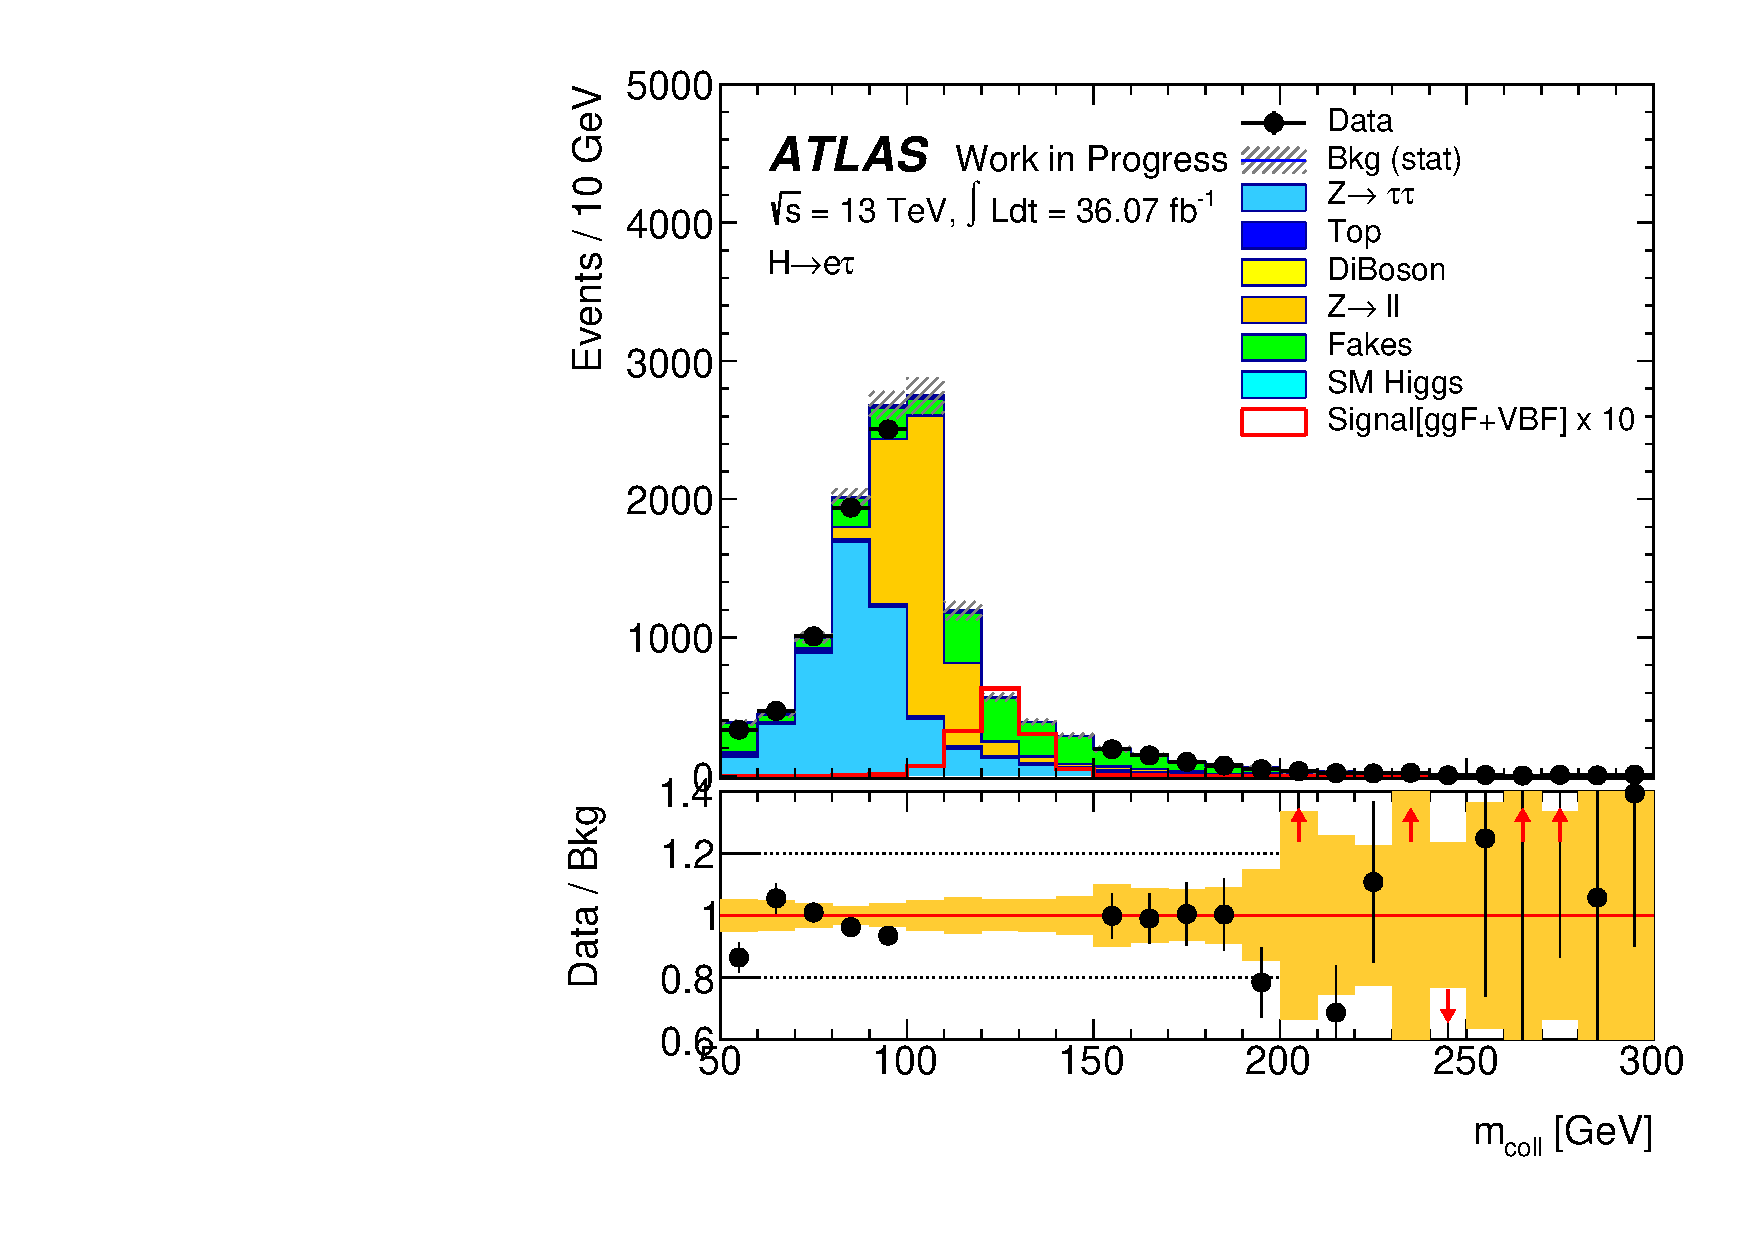
\includegraphics[width=.40\textwidth,height=.40\textheight,type=png,ext=.pdf,read=.pdf]{/afs/cern.ch/user/a/atpathak/afswork/private/xTauFramework/xTauFramework/test_candidacy_20Nov2017/Plots/plots/etau-CutTauMTSR2-collMassBL-lin}\\
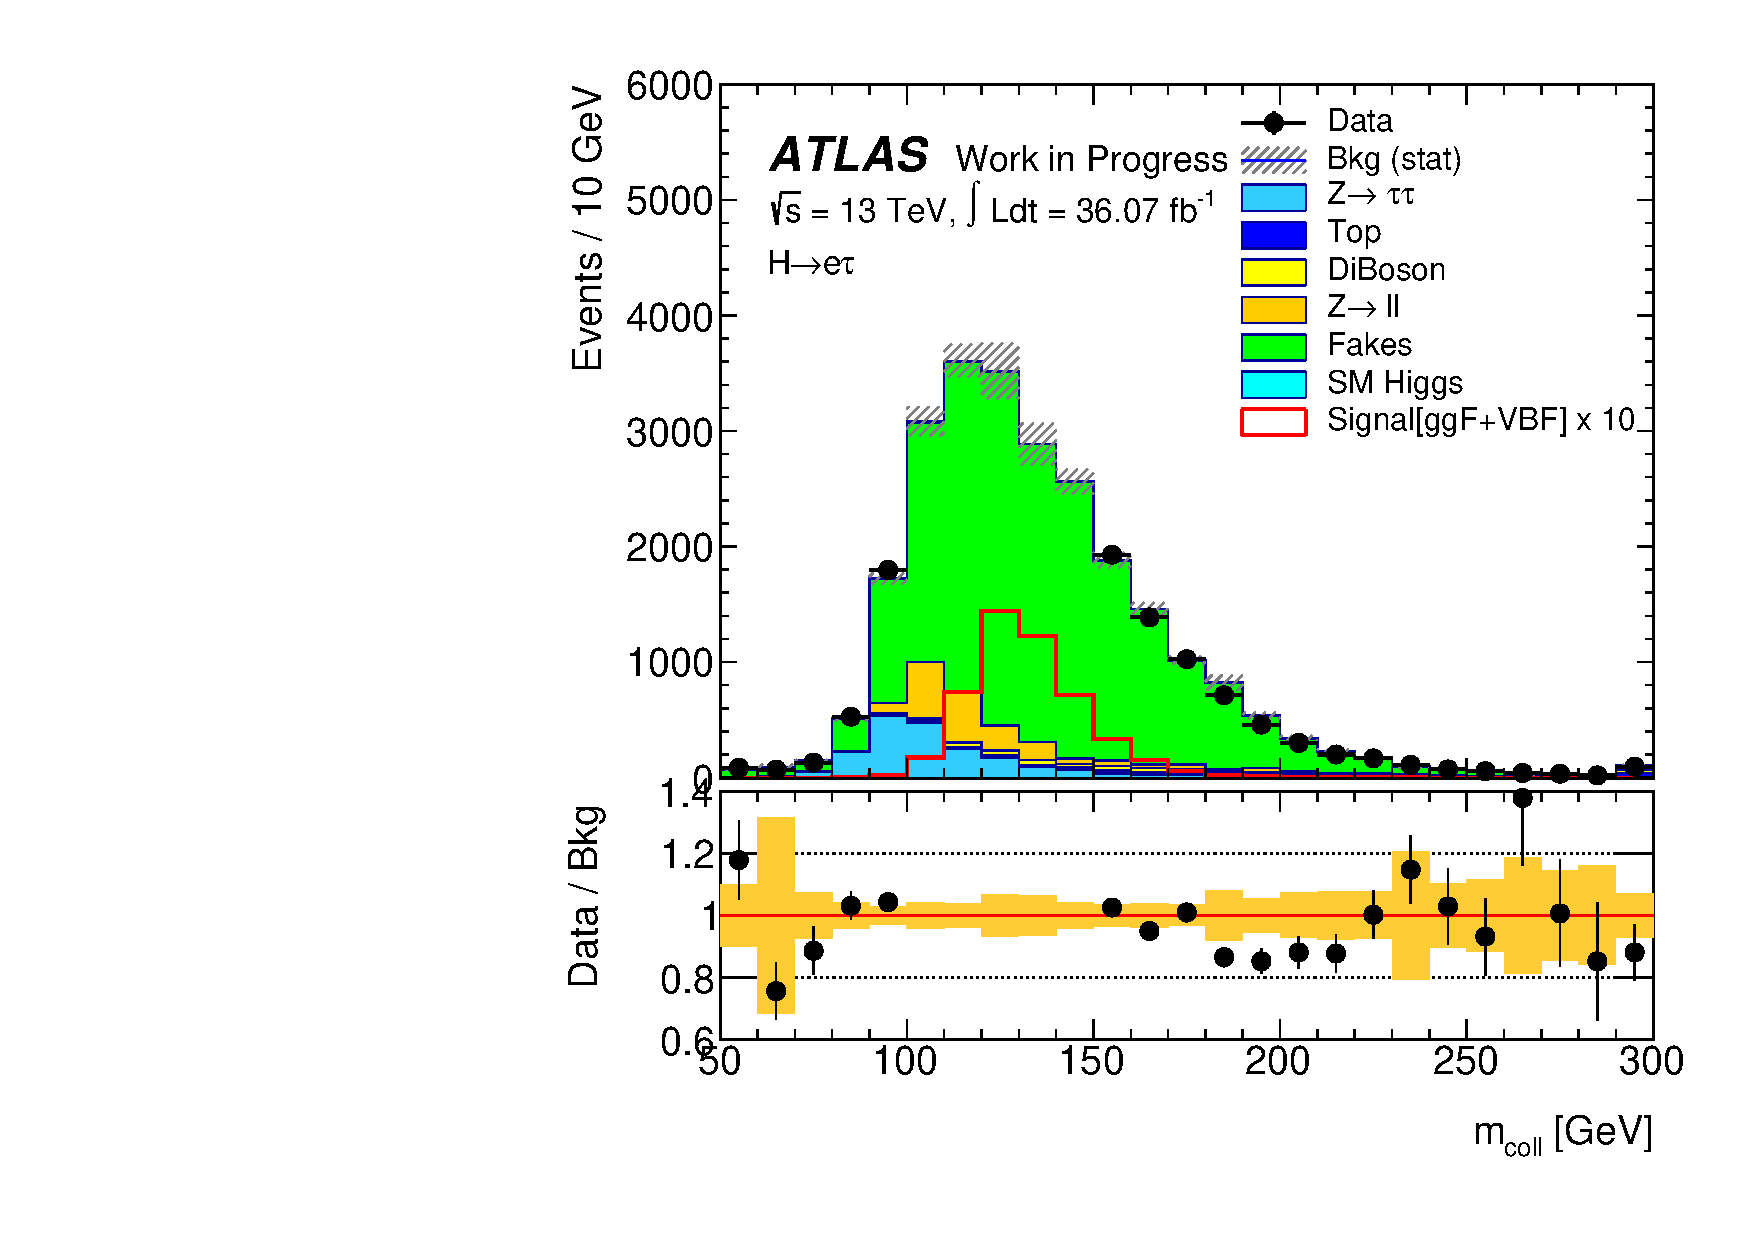
\includegraphics[width=.40\textwidth,height=.40\textheight,type=png,ext=.pdf,read=.pdf]{/afs/cern.ch/user/a/atpathak/afswork/private/xTauFramework/xTauFramework/test_candidacy_20Nov2017/Plots/plots/etau-CutTauPtSR3-collMassBL-lin}  
\end{center}
\end{normalsize}

\end {frame}
%------------------------------------------------
\begin{frame}
\frametitle{ collinear mass in $H\to \mu\tau_{had}$ }
\begin{normalsize}
\begin{center}
SR1 and SR2 (left to right) SR3(Below)
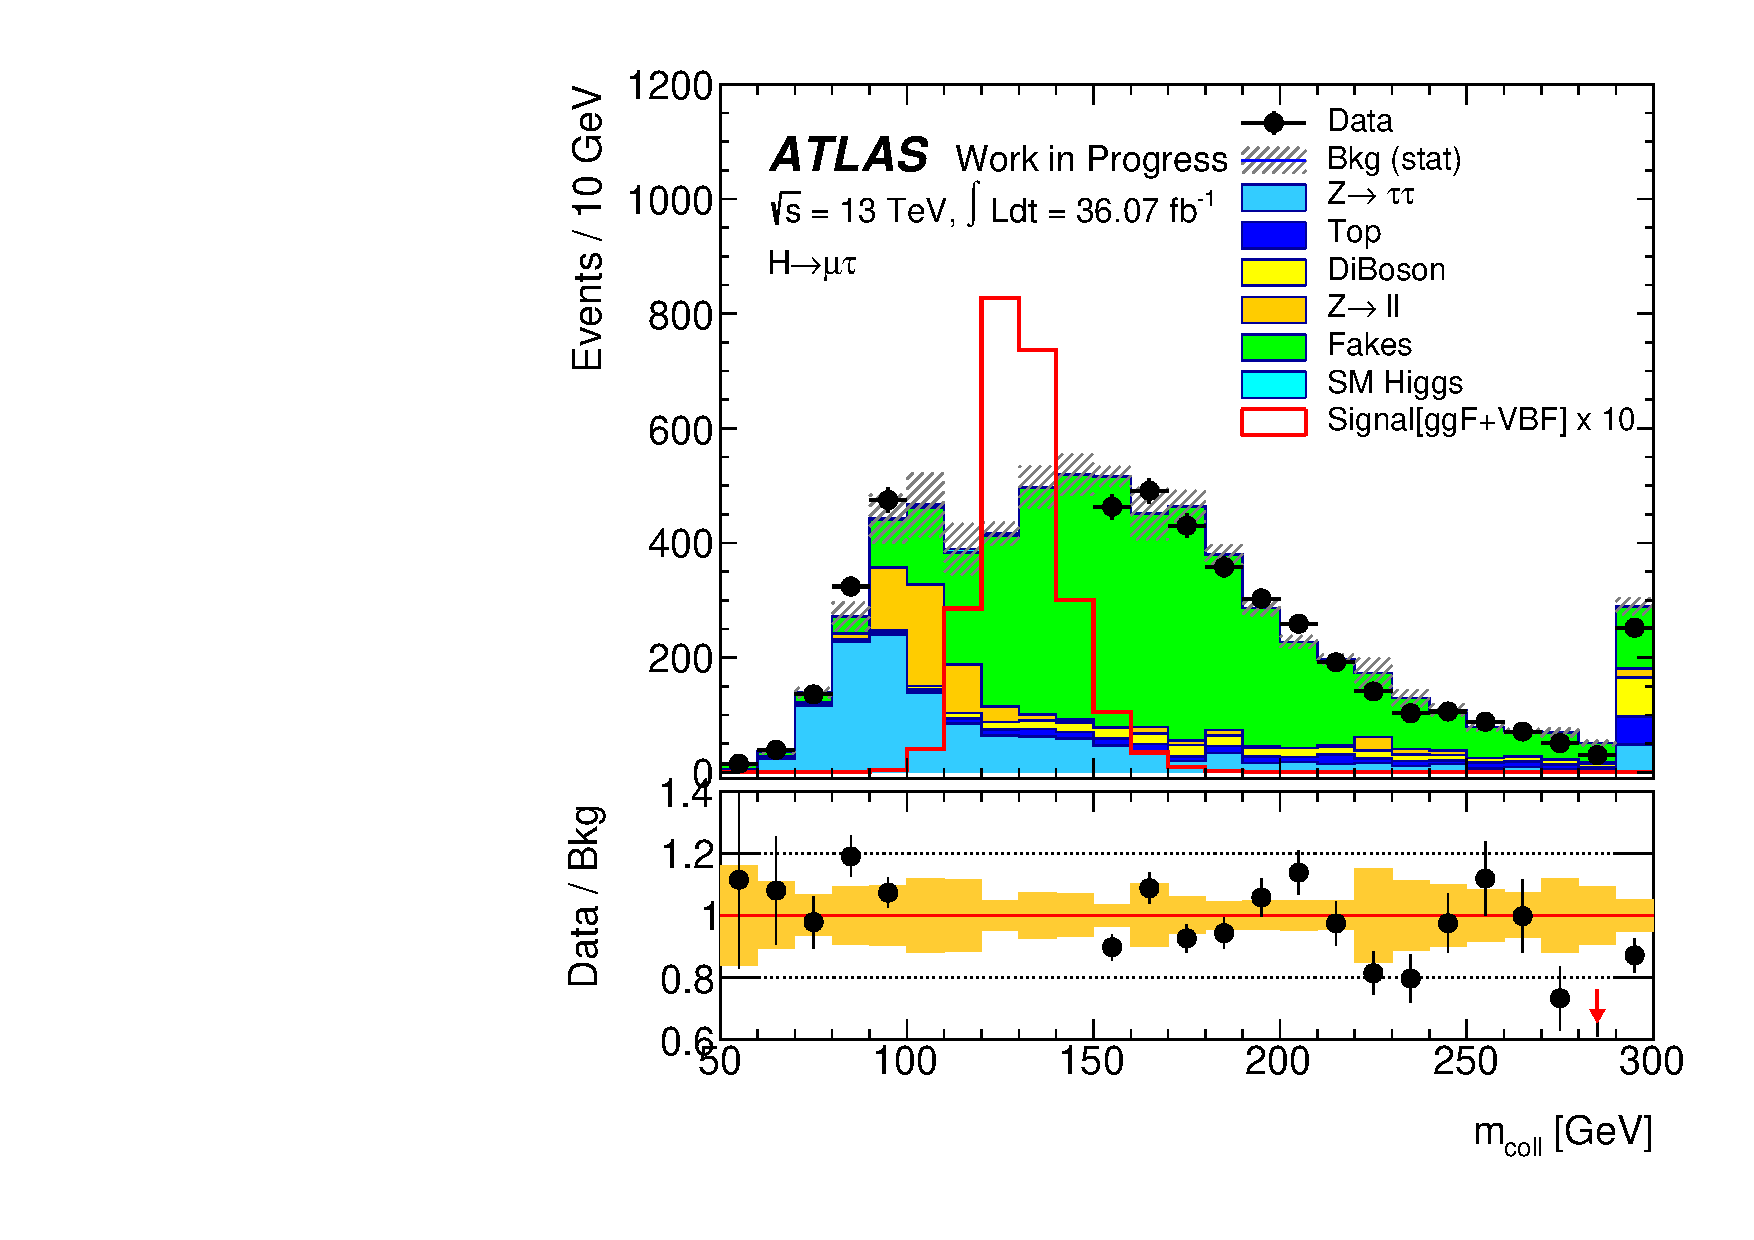
\includegraphics[width=.40\textwidth,height=.40\textheight,type=png,ext=.pdf,read=.pdf]{/afs/cern.ch/user/a/atpathak/afswork/private/xTauFramework/xTauFramework/test_candidacy_20Nov2017/Plots/plots/mtau-CutTauMTSR1-collMassBL-lin}
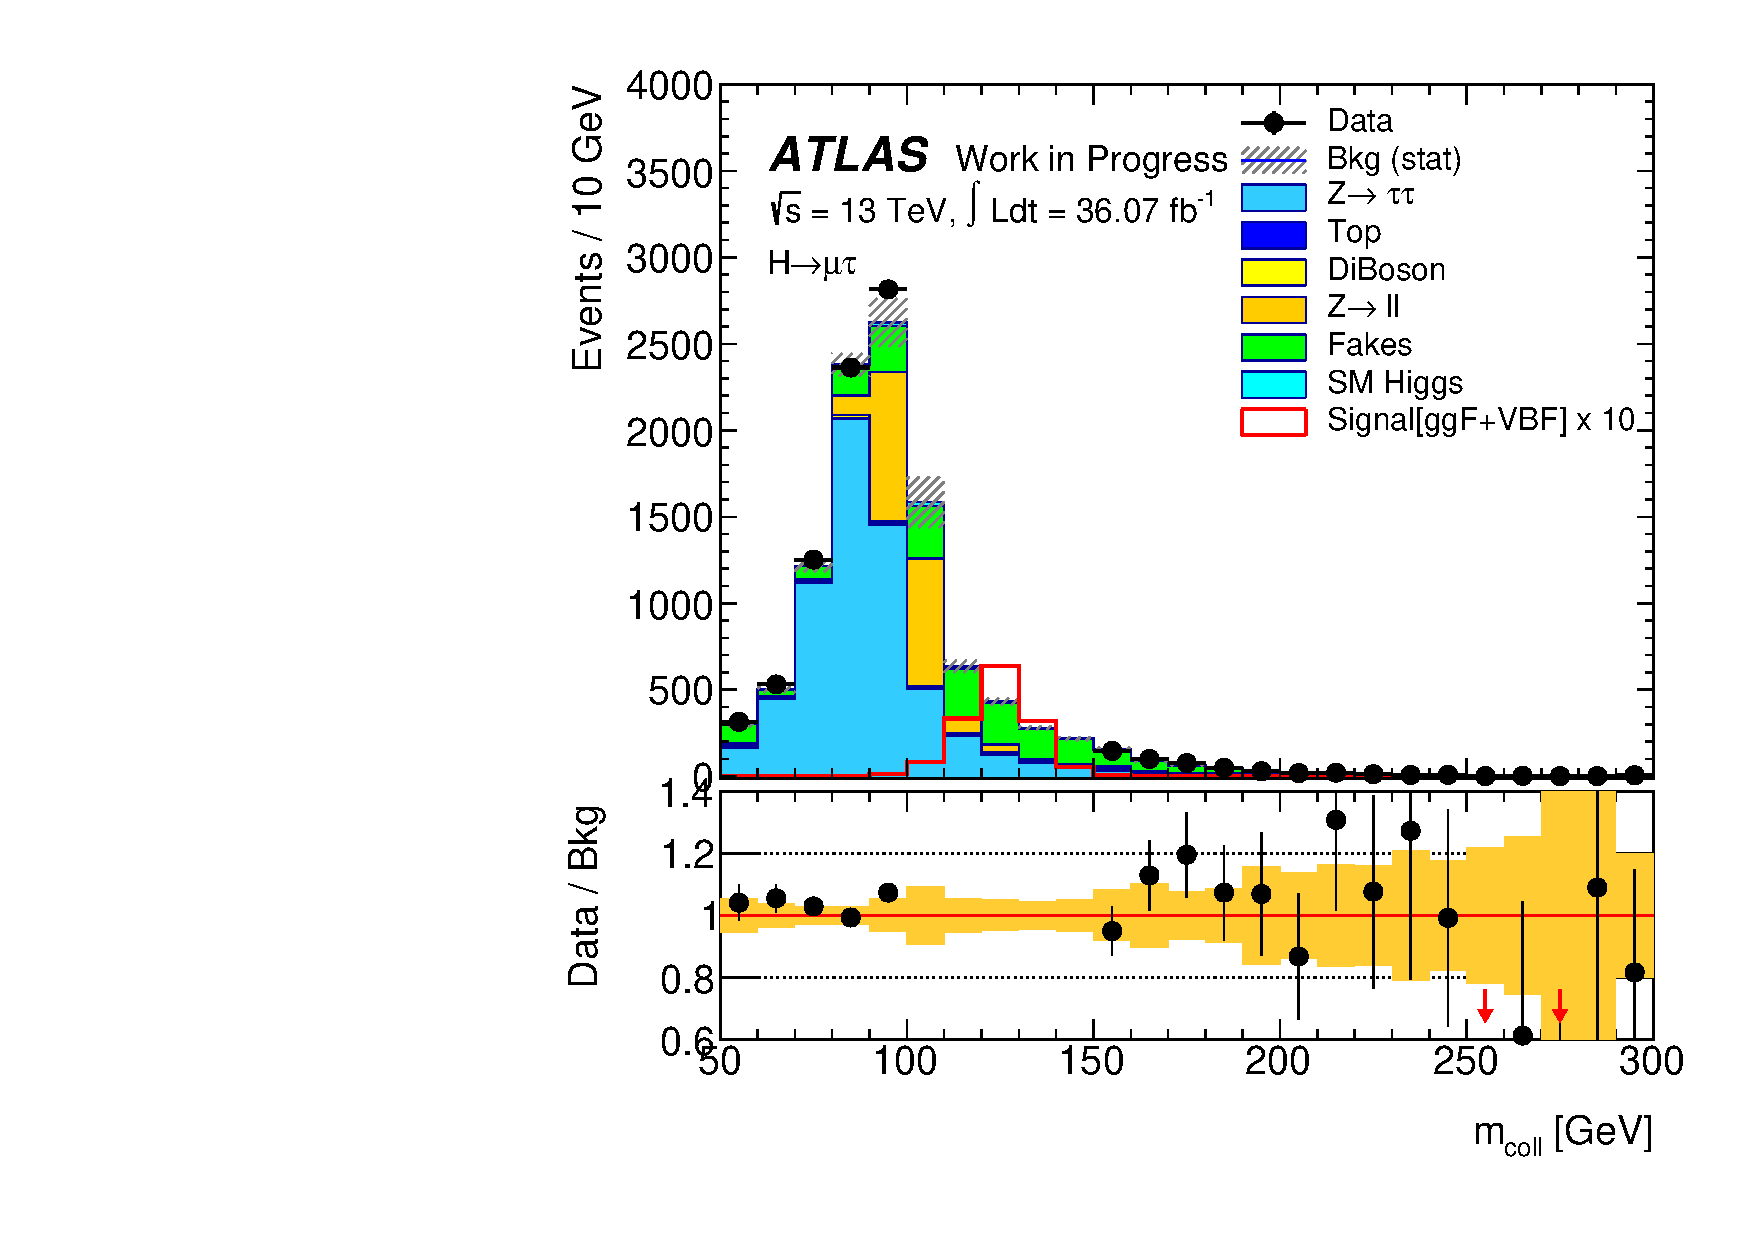
\includegraphics[width=.40\textwidth,height=.40\textheight,type=png,ext=.pdf,read=.pdf]{/afs/cern.ch/user/a/atpathak/afswork/private/xTauFramework/xTauFramework/test_candidacy_20Nov2017/Plots/plots/mtau-CutTauMTSR2-collMassBL-lin}\\
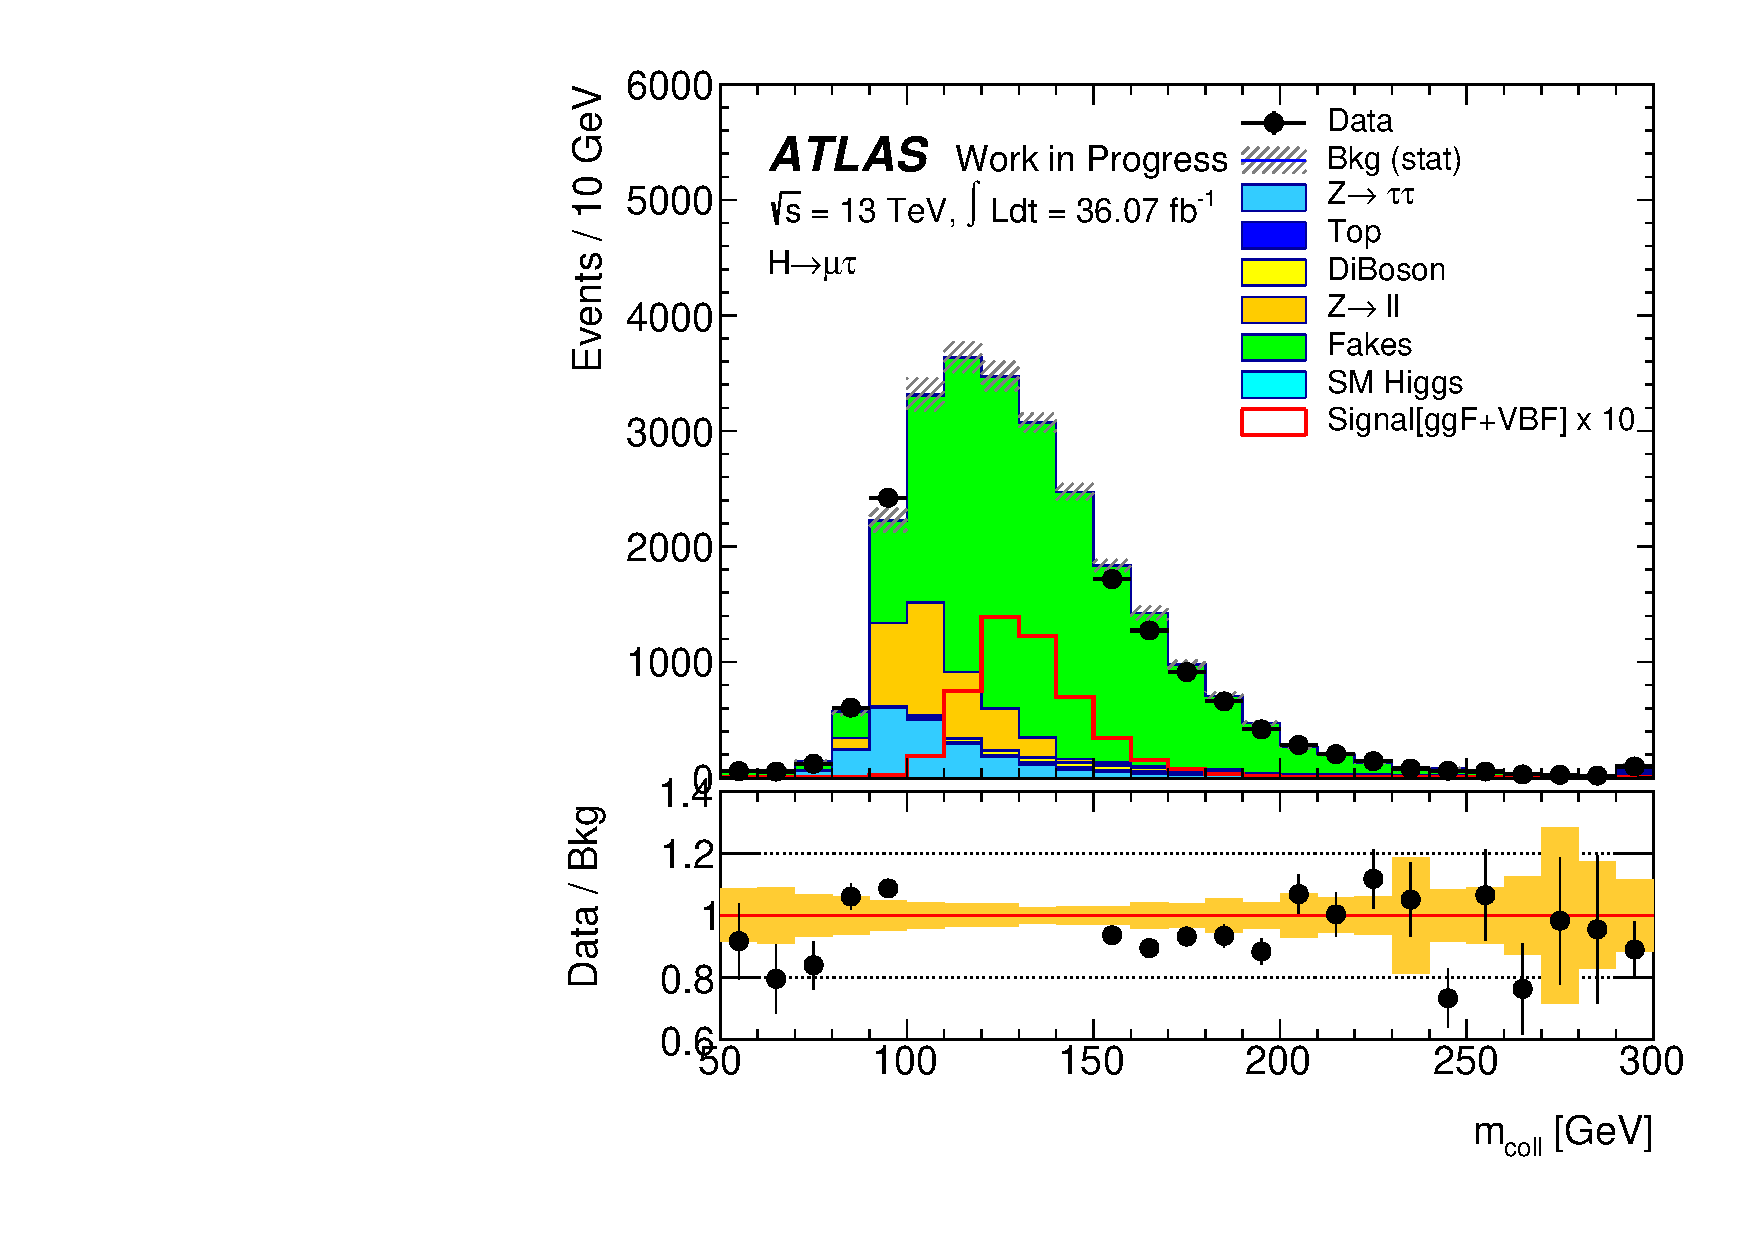
\includegraphics[width=.40\textwidth,height=.40\textheight,type=png,ext=.pdf,read=.pdf]{/afs/cern.ch/user/a/atpathak/afswork/private/xTauFramework/xTauFramework/test_candidacy_20Nov2017/Plots/plots/mtau-CutTauPtSR3-collMassBL-lin}  
\end{center}
\end{normalsize}

\end {frame}
\end{document}
%-------------------------------------------------
\begin{frame}
\frametitle{List of Algorithm Names :}
\begin{itemize}
\item Full Detector : 
\end{itemize}
\vspace*{0.5cm} 
\begin{table}

{\scalebox{.36}{
\begin{tabular}{|l|c|c|c|c|c|c|c|}\hline\hline
                           
Detector  &              Si Pre-                       &             SP                                     &              Pattern                                &         Ambiguity                                 &          Back-                           &     Primary              & ITk General                    \\ 
               &          Processing                     &        formation                              &          recognition                             &         Solution                                    &           tracking                      &      Vertex               &                                        \\ \hline
ITk          &  InDetSCT\_Clusterization      & InDetSiTrackerSpacePointFinder   & InDetSiSpTrackFinderSLHC              &  InDetAmbiguitySolverSLHC               &               $-$                        &  InDetPriVxFinder  & InDetCaloClusterROISelector \\
               &  InDetPixelClusterization        &                                                      &                                                         &                                                          &               $-$                         &                              & InDetCopyAlg                        \\
               &                                                &                                                      &                                                         &                                                          &               $-$                          &                             & InDetTrackCollectionMerger \\
               &                                                &                                                      &                                                         &                                                          &               $-$                          &                             & InDetTrackParticles              \\
               &                                                &                                                      &                                                         &                                                          &               $-$                          &                             & InDetVxLinkSetter                 \\
               &                                                &                                                      &                                                         &                                                          &               $-$                          &                             & InDetRecStatistics           \\          \hline\hline

\end{tabular}
}}
\end{table}
\vspace*{1cm}
\end{frame}
%-------------------------------------------------
\begin{frame}
\frametitle{List of Algorithm Names :}
\begin{itemize}
\item Full Detector : 
\end{itemize}
\vspace*{0.5cm} 
\begin{table}

{\scalebox{.29}{
\begin{tabular}{|l|c|c|c|c|c|c|c|}\hline\hline
Detector  &              Si Pre-                       &             SP                                     &              Pattern                                &         Ambiguity                                 &          Back-                                  &     Primary             & ITk General                    \\ 
               &          Processing                     &        formation                              &          recognition                             &         Solution                                    &           tracking                              &      Vertex              &                                        \\ \hline
Run 2      &  InDetSCT\_Clusterization +  &  InDetSiTrackerSpacePointFinder  & InDetSiSpTrackFinder                      & InDetAmbiguitySolver                      &  InDetTRT\_RIO\_Maker                 & InDetPriVxFinder  &InDetCaloClusterROISelector \\
               &  InDetPixelClusterization        &                                                     & InDetSiSpTrackFinderForwardTracks& InDetAmbiguitySolverForwardTracks& InDetTRT\_Extension                    &                             &InDetSegmentPRD\_Association\\
                &                                               &                                                      &                                                         &                                                          & InDetExtensionProcessor               &                             &InDetTRTonly\_PRD\_Association \\
                &                                               &                                                      &                                                         &                                                          & InDetTRT\_TrackSegmentsFinder   &                             &InDetPRD\_AssociationForwardTracks  \\                           
                &                                               &                                                      &                                                         &                                                          & InDetTRT\_SeededTrackFinde          &                            & InDetTrackCollectionMerger \\
                &                                               &                                                      &                                                         &                                                          & InDetTRT\_SeededAmbiguitySolver  &                             & InDetTrackSlimmer \\
                &                                               &                                                      &                                                         &                                                          & InDetTRT\_StandaloneTrackFinder   &                              & InDetTrackParticles \\
                &                                               &                                                      &                                                         &                                                          &                                                          &                              & InDetForwardTrackParticles \\
                &                                               &                                                      &                                                         &                                                          &                                                          &                              & InDetVxLinkSetter \\
                &                                               &                                                      &                                                         &                                                          &                                                          &                               & InDetBCM\_ZeroSuppression \\
                &                                               &                                                      &                                                         &                                                          &                                                          &                                &InDetCosmicsEventPhase \\
                &                                               &                                                      &                                                         &                                                          &                                                          &                                &InDetRecStatistics \\
\hline
\end{tabular}
}}
\end{table}
\vspace*{1cm}
\end{frame}
\end{document}
%------------------------------------------------
\begin{frame}

\begin{normalsize}
\begin{center}
\includegraphics[width=.50\textwidth,height=.50\textheight,type=png,ext=.pdf,read=.pdf]{/afs/cern.ch/work/a/atpathak/public/Pixel/LFV_Plots/Plots_project_New/Angle_Vis_neutrino_cut1_1}
\includegraphics[width=.50\textwidth,height=.50\textheight,type=png,ext=.pdf,read=.pdf]{/afs/cern.ch/work/a/atpathak/public/Pixel/LFV_Plots/Plots_project_New/Angle_Vis_neutrino_cut2_1}\\
\includegraphics[width=.45\textwidth,height=.45\textheight,type=png,ext=.pdf,read=.pdf]{/afs/cern.ch/work/a/atpathak/public/Pixel/LFV_Plots/Plots_project_New/Angle_Vis_neutrino_cut3_1}  
\end{center}
\end{normalsize}

\end {frame}
%------------------------------------------------
\begin{frame}

\begin{normalsize}
\begin{center}
\includegraphics[width=.50\textwidth,height=.50\textheight,type=png,ext=.pdf,read=.pdf]{/afs/cern.ch/work/a/atpathak/public/Pixel/LFV_Plots/Plots_project_New/Angle_Vis_neutrino_cut1_2}
\includegraphics[width=.50\textwidth,height=.50\textheight,type=png,ext=.pdf,read=.pdf]{/afs/cern.ch/work/a/atpathak/public/Pixel/LFV_Plots/Plots_project_New/Angle_Vis_neutrino_cut2_2}\\
\includegraphics[width=.45\textwidth,height=.45\textheight,type=png,ext=.pdf,read=.pdf]{/afs/cern.ch/work/a/atpathak/public/Pixel/LFV_Plots/Plots_project_New/Angle_Vis_neutrino_cut3_2}  
\end{center}
\end{normalsize}

\end {frame}
%------------------------------------------------
\begin{frame}

\begin{normalsize}
\begin{center}
\includegraphics[width=.50\textwidth,height=.50\textheight,type=png,ext=.pdf,read=.pdf]{/afs/cern.ch/work/a/atpathak/public/Pixel/LFV_Plots/Plots_project_New/Angle_Vis_neutrino_cut1_3}
\includegraphics[width=.50\textwidth,height=.50\textheight,type=png,ext=.pdf,read=.pdf]{/afs/cern.ch/work/a/atpathak/public/Pixel/LFV_Plots/Plots_project_New/Angle_Vis_neutrino_cut2_3}\\
\includegraphics[width=.45\textwidth,height=.45\textheight,type=png,ext=.pdf,read=.pdf]{/afs/cern.ch/work/a/atpathak/public/Pixel/LFV_Plots/Plots_project_New/Angle_Vis_neutrino_cut3_3}  
\end{center}
\end{normalsize}

\end {frame}
%------------------------------------------------
\begin{frame}

\begin{normalsize}
\begin{center}
\includegraphics[width=.50\textwidth,height=.50\textheight,type=png,ext=.pdf,read=.pdf]{/afs/cern.ch/work/a/atpathak/public/Pixel/LFV_Plots/Plots_project_New/Angle_Vis_neutrino_cut1_4}
\includegraphics[width=.50\textwidth,height=.50\textheight,type=png,ext=.pdf,read=.pdf]{/afs/cern.ch/work/a/atpathak/public/Pixel/LFV_Plots/Plots_project_New/Angle_Vis_neutrino_cut2_4}\\
\includegraphics[width=.45\textwidth,height=.45\textheight,type=png,ext=.pdf,read=.pdf]{/afs/cern.ch/work/a/atpathak/public/Pixel/LFV_Plots/Plots_project_New/Angle_Vis_neutrino_cut3_4}  
\end{center}
\end{normalsize}

\end {frame}
%------------------------------------------------
\begin{frame}

\begin{normalsize}
\begin{center}
\includegraphics[width=.50\textwidth,height=.50\textheight,type=png,ext=.pdf,read=.pdf]{/afs/cern.ch/work/a/atpathak/public/Pixel/LFV_Plots/Plots_project_New/Angle_Vis_neutrino_cut1_5}
\includegraphics[width=.50\textwidth,height=.50\textheight,type=png,ext=.pdf,read=.pdf]{/afs/cern.ch/work/a/atpathak/public/Pixel/LFV_Plots/Plots_project_New/Angle_Vis_neutrino_cut2_5}\\
\includegraphics[width=.45\textwidth,height=.45\textheight,type=png,ext=.pdf,read=.pdf]{/afs/cern.ch/work/a/atpathak/public/Pixel/LFV_Plots/Plots_project_New/Angle_Vis_neutrino_cut3_5}  
\end{center}
\end{normalsize}

\end {frame}
%------------------------------------------------
\begin{frame}

\begin{normalsize}
\begin{center}
\includegraphics[width=.50\textwidth,height=.50\textheight,type=png,ext=.pdf,read=.pdf]{/afs/cern.ch/work/a/atpathak/public/Pixel/LFV_Plots/Plots_project_New/Angle_Vis_neutrino_cut1_6}
\includegraphics[width=.50\textwidth,height=.50\textheight,type=png,ext=.pdf,read=.pdf]{/afs/cern.ch/work/a/atpathak/public/Pixel/LFV_Plots/Plots_project_New/Angle_Vis_neutrino_cut2_6}\\
\includegraphics[width=.45\textwidth,height=.45\textheight,type=png,ext=.pdf,read=.pdf]{/afs/cern.ch/work/a/atpathak/public/Pixel/LFV_Plots/Plots_project_New/Angle_Vis_neutrino_cut3_6}  
\end{center}
\end{normalsize}

\end {frame}
%------------------------------------------------
\begin{frame}

\begin{normalsize}
\begin{center}
\includegraphics[width=.50\textwidth,height=.50\textheight,type=png,ext=.pdf,read=.pdf]{/afs/cern.ch/work/a/atpathak/public/Pixel/LFV_Plots/Plots_project_New/Angle_Vis_neutrino_cut1_7}
\includegraphics[width=.50\textwidth,height=.50\textheight,type=png,ext=.pdf,read=.pdf]{/afs/cern.ch/work/a/atpathak/public/Pixel/LFV_Plots/Plots_project_New/Angle_Vis_neutrino_cut2_7}\\
\includegraphics[width=.45\textwidth,height=.45\textheight,type=png,ext=.pdf,read=.pdf]{/afs/cern.ch/work/a/atpathak/public/Pixel/LFV_Plots/Plots_project_New/Angle_Vis_neutrino_cut3_7}  
\end{center}
\end{normalsize}

\end {frame}
%------------------------------------------------
\begin{frame}

\begin{normalsize}
\begin{center}
\includegraphics[width=.50\textwidth,height=.50\textheight,type=png,ext=.pdf,read=.pdf]{/afs/cern.ch/work/a/atpathak/public/Pixel/LFV_Plots/Plots_project_New/Angle_Vis_neutrino_cut1_8}
\includegraphics[width=.50\textwidth,height=.50\textheight,type=png,ext=.pdf,read=.pdf]{/afs/cern.ch/work/a/atpathak/public/Pixel/LFV_Plots/Plots_project_New/Angle_Vis_neutrino_cut2_8}\\
\includegraphics[width=.45\textwidth,height=.45\textheight,type=png,ext=.pdf,read=.pdf]{/afs/cern.ch/work/a/atpathak/public/Pixel/LFV_Plots/Plots_project_New/Angle_Vis_neutrino_cut3_8}  
\end{center}
\end{normalsize}

\end {frame}
%------------------------------------------------
\begin{frame}

\begin{normalsize}
\begin{center}
\includegraphics[width=.50\textwidth,height=.50\textheight,type=png,ext=.pdf,read=.pdf]{/afs/cern.ch/work/a/atpathak/public/Pixel/LFV_Plots/Plots_project_New/Angle_Vis_neutrino_cut1_9}
\includegraphics[width=.50\textwidth,height=.50\textheight,type=png,ext=.pdf,read=.pdf]{/afs/cern.ch/work/a/atpathak/public/Pixel/LFV_Plots/Plots_project_New/Angle_Vis_neutrino_cut2_9}\\
\includegraphics[width=.45\textwidth,height=.45\textheight,type=png,ext=.pdf,read=.pdf]{/afs/cern.ch/work/a/atpathak/public/Pixel/LFV_Plots/Plots_project_New/Angle_Vis_neutrino_cut3_9}  
\end{center}
\end{normalsize}

\end {frame}
%------------------------------------------------
\begin{frame}

\begin{normalsize}
\begin{center}
\includegraphics[width=.50\textwidth,height=.50\textheight,type=png,ext=.pdf,read=.pdf]{/afs/cern.ch/work/a/atpathak/public/Pixel/LFV_Plots/Plots_project_New/Angle_Vis_neutrino_cut1_10}
\includegraphics[width=.50\textwidth,height=.50\textheight,type=png,ext=.pdf,read=.pdf]{/afs/cern.ch/work/a/atpathak/public/Pixel/LFV_Plots/Plots_project_New/Angle_Vis_neutrino_cut2_10}\\
\includegraphics[width=.45\textwidth,height=.45\textheight,type=png,ext=.pdf,read=.pdf]{/afs/cern.ch/work/a/atpathak/public/Pixel/LFV_Plots/Plots_project_New/Angle_Vis_neutrino_cut3_10}  
\end{center}
\end{normalsize}

\end {frame}
\end{document}
\fi
%------------------------------------------------
\iffalse
\begin{frame}
\frametitle{  $H\to \tau_{lep}\tau_{had}$ }
\begin{normalsize}
\begin{center}
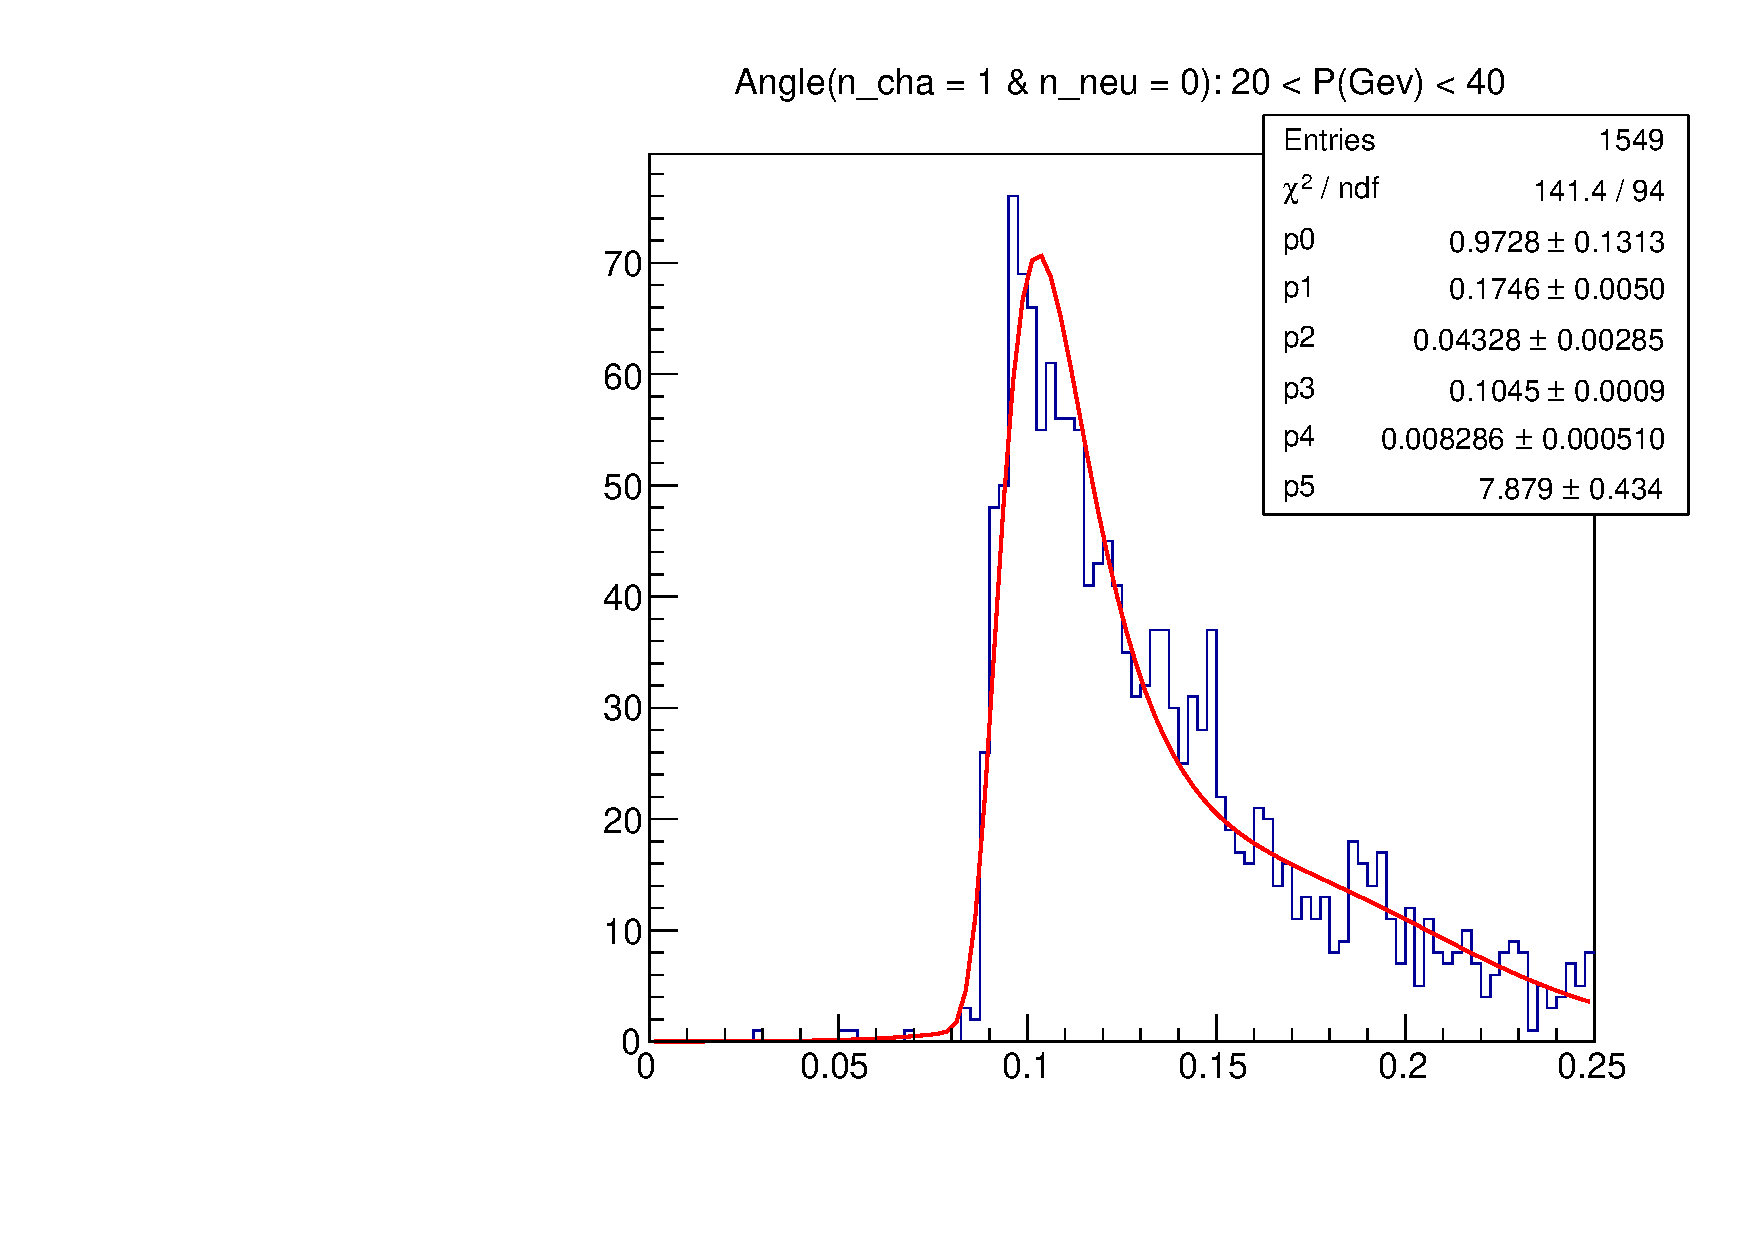
\includegraphics[width=.50\textwidth,height=.50\textheight,type=png,ext=.pdf,read=.pdf]{/afs/cern.ch/work/a/atpathak/public/Pixel/LFV_Plots/Plots_Fit_tautau/Angle_Vis_neutrino_decay1_Fit_1}
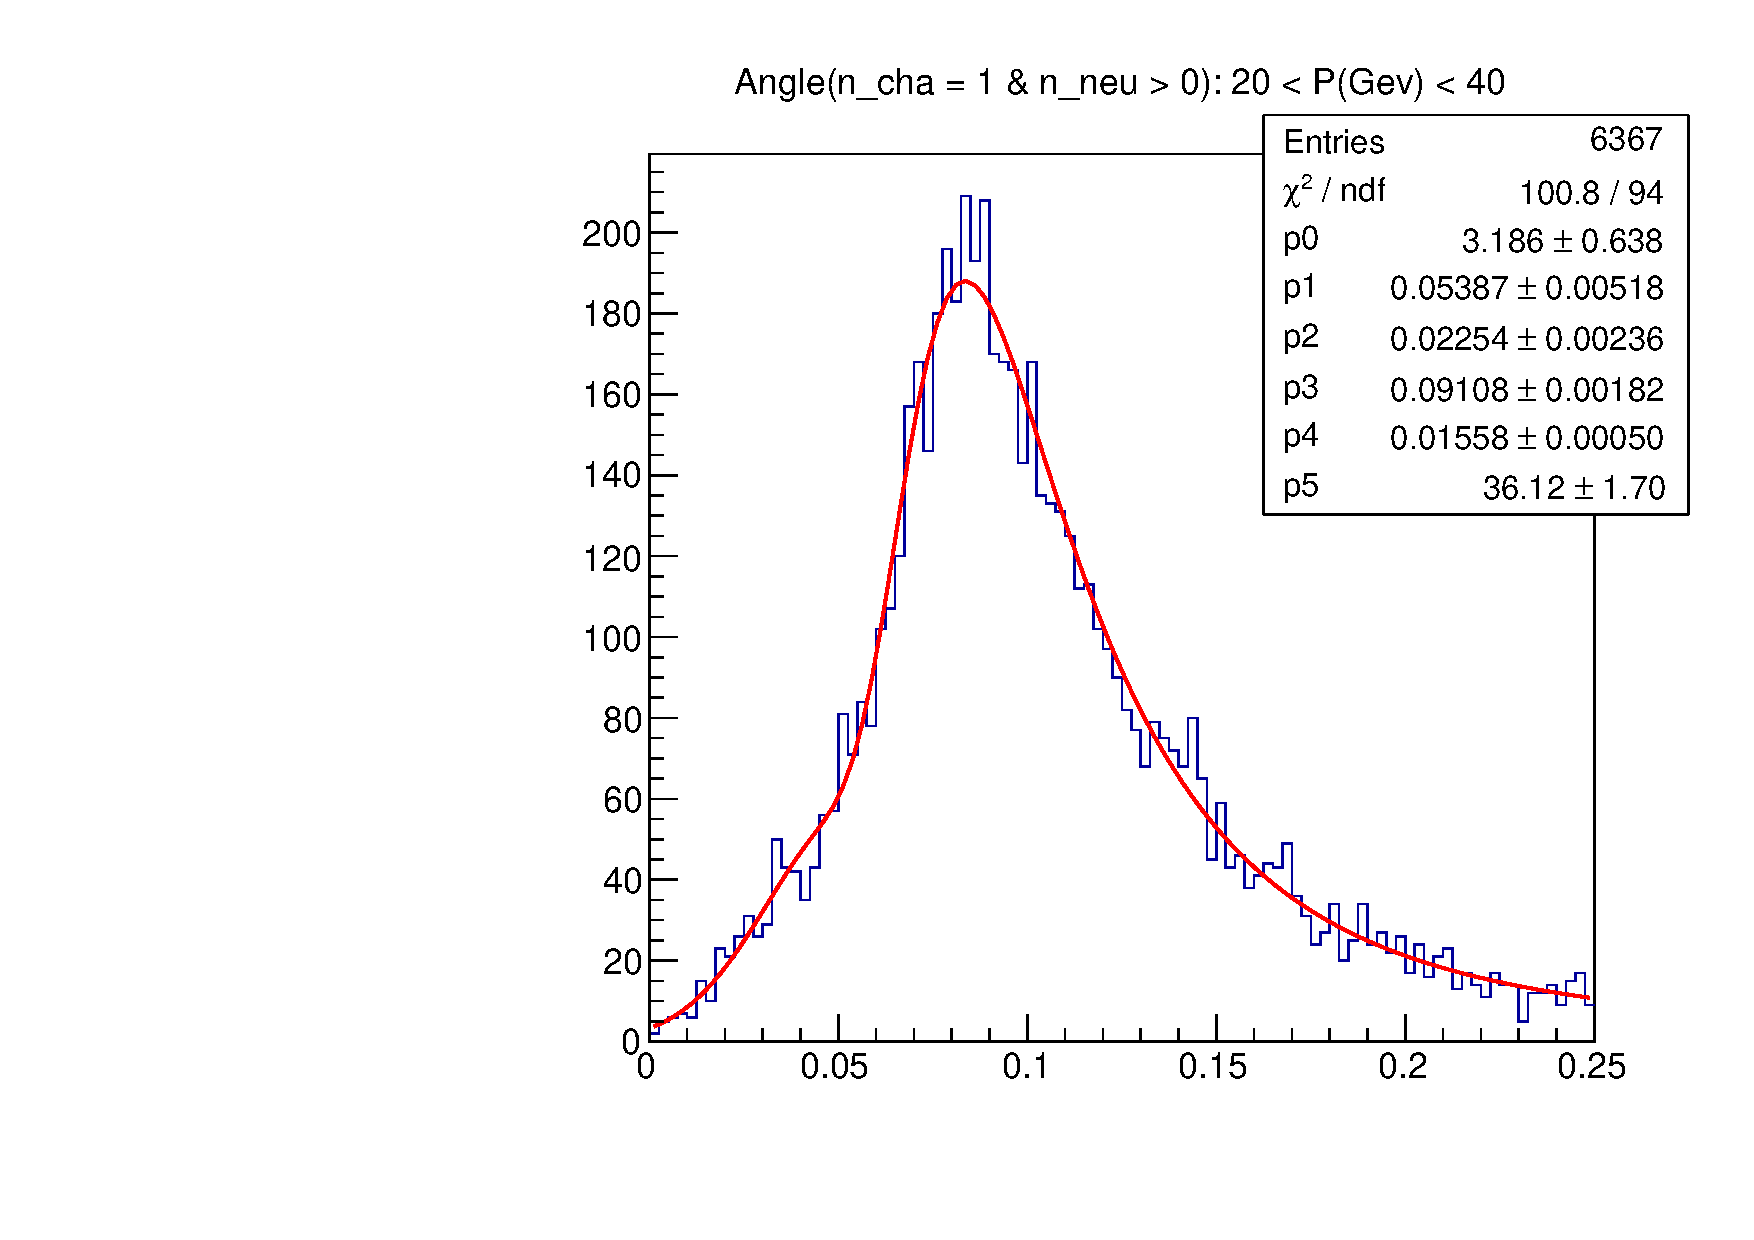
\includegraphics[width=.50\textwidth,height=.50\textheight,type=png,ext=.pdf,read=.pdf]{/afs/cern.ch/work/a/atpathak/public/Pixel/LFV_Plots/Plots_Fit_tautau/Angle_Vis_neutrino_decay2_Fit_1}\\
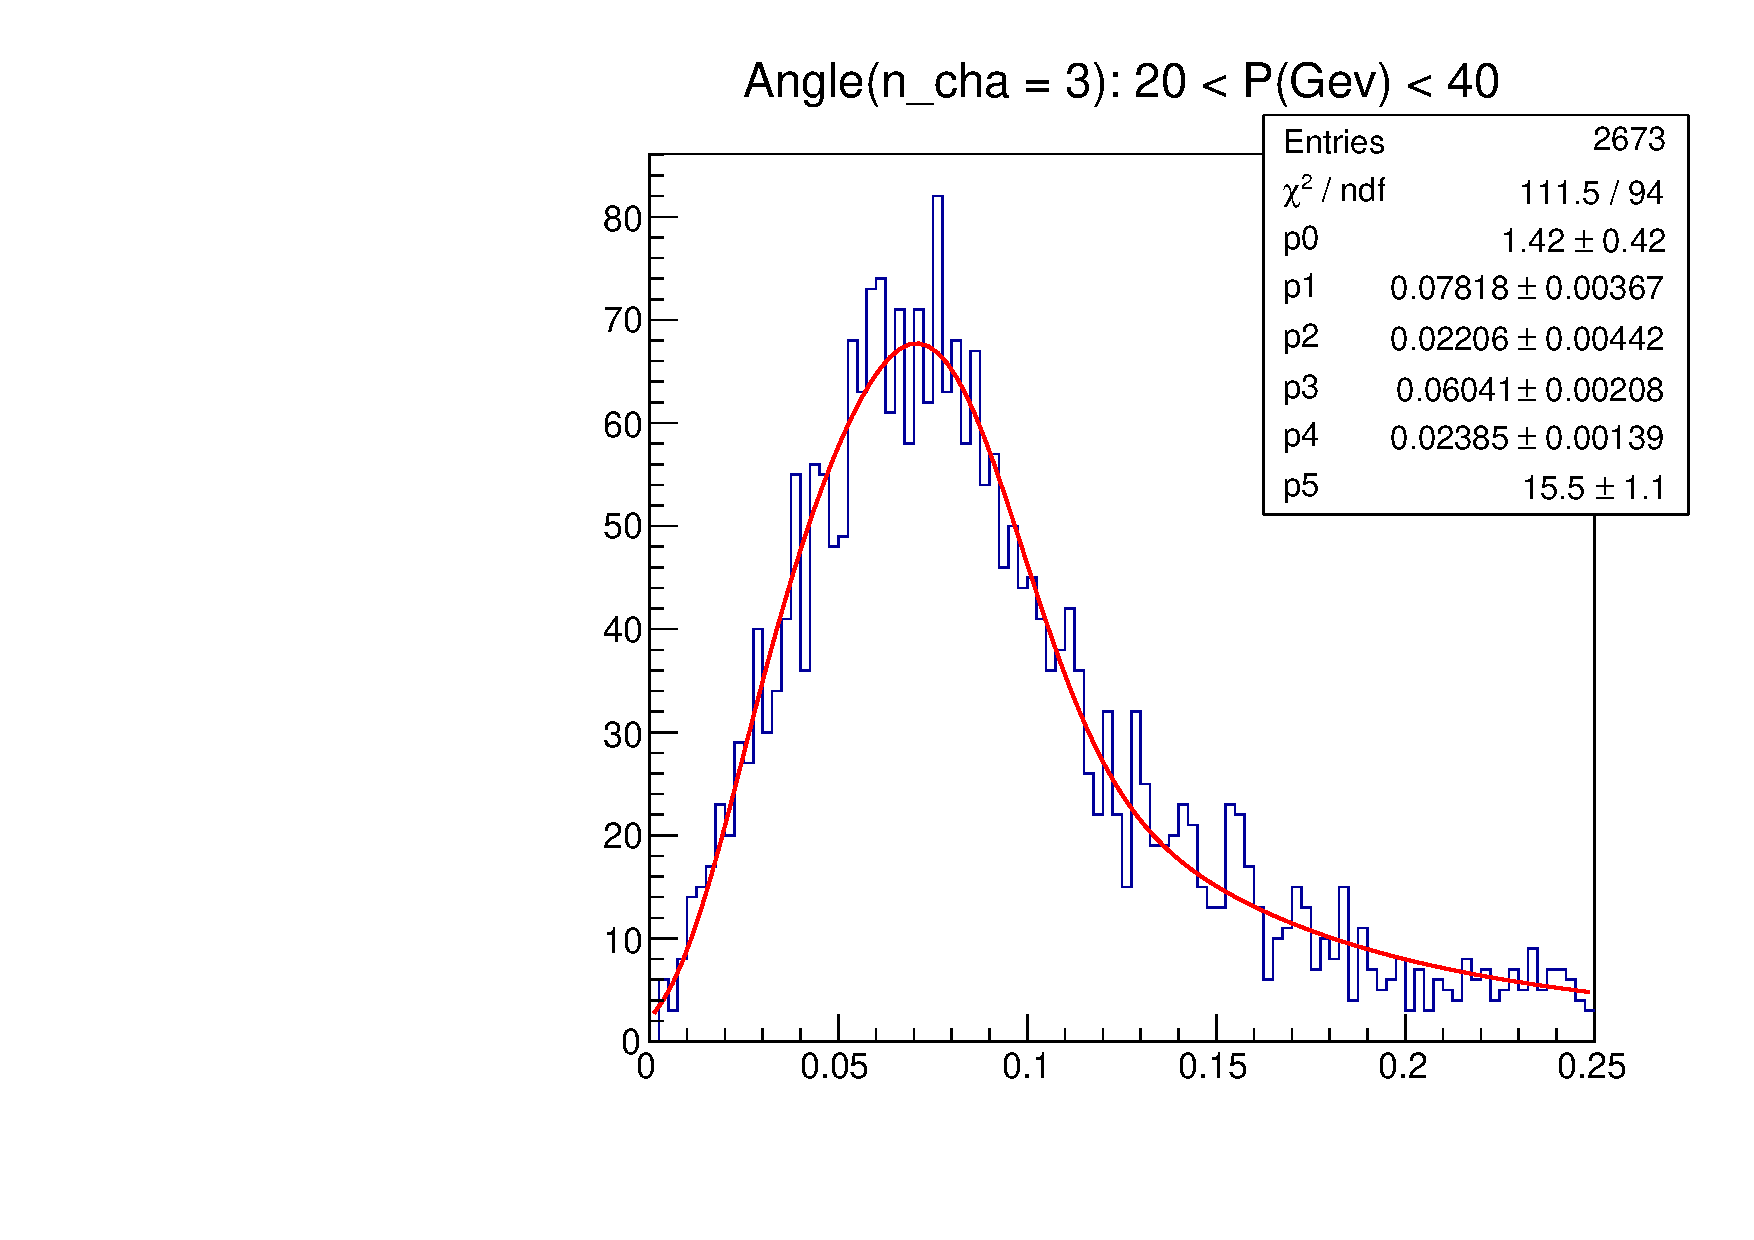
\includegraphics[width=.40\textwidth,height=.40\textheight,type=png,ext=.pdf,read=.pdf]{/afs/cern.ch/work/a/atpathak/public/Pixel/LFV_Plots/Plots_Fit_tautau/Angle_Vis_neutrino_decay3_Fit_1}  
\end{center}
\end{normalsize}

\end {frame}
%------------------------------------------------
\begin{frame}

\begin{normalsize}
\begin{center}
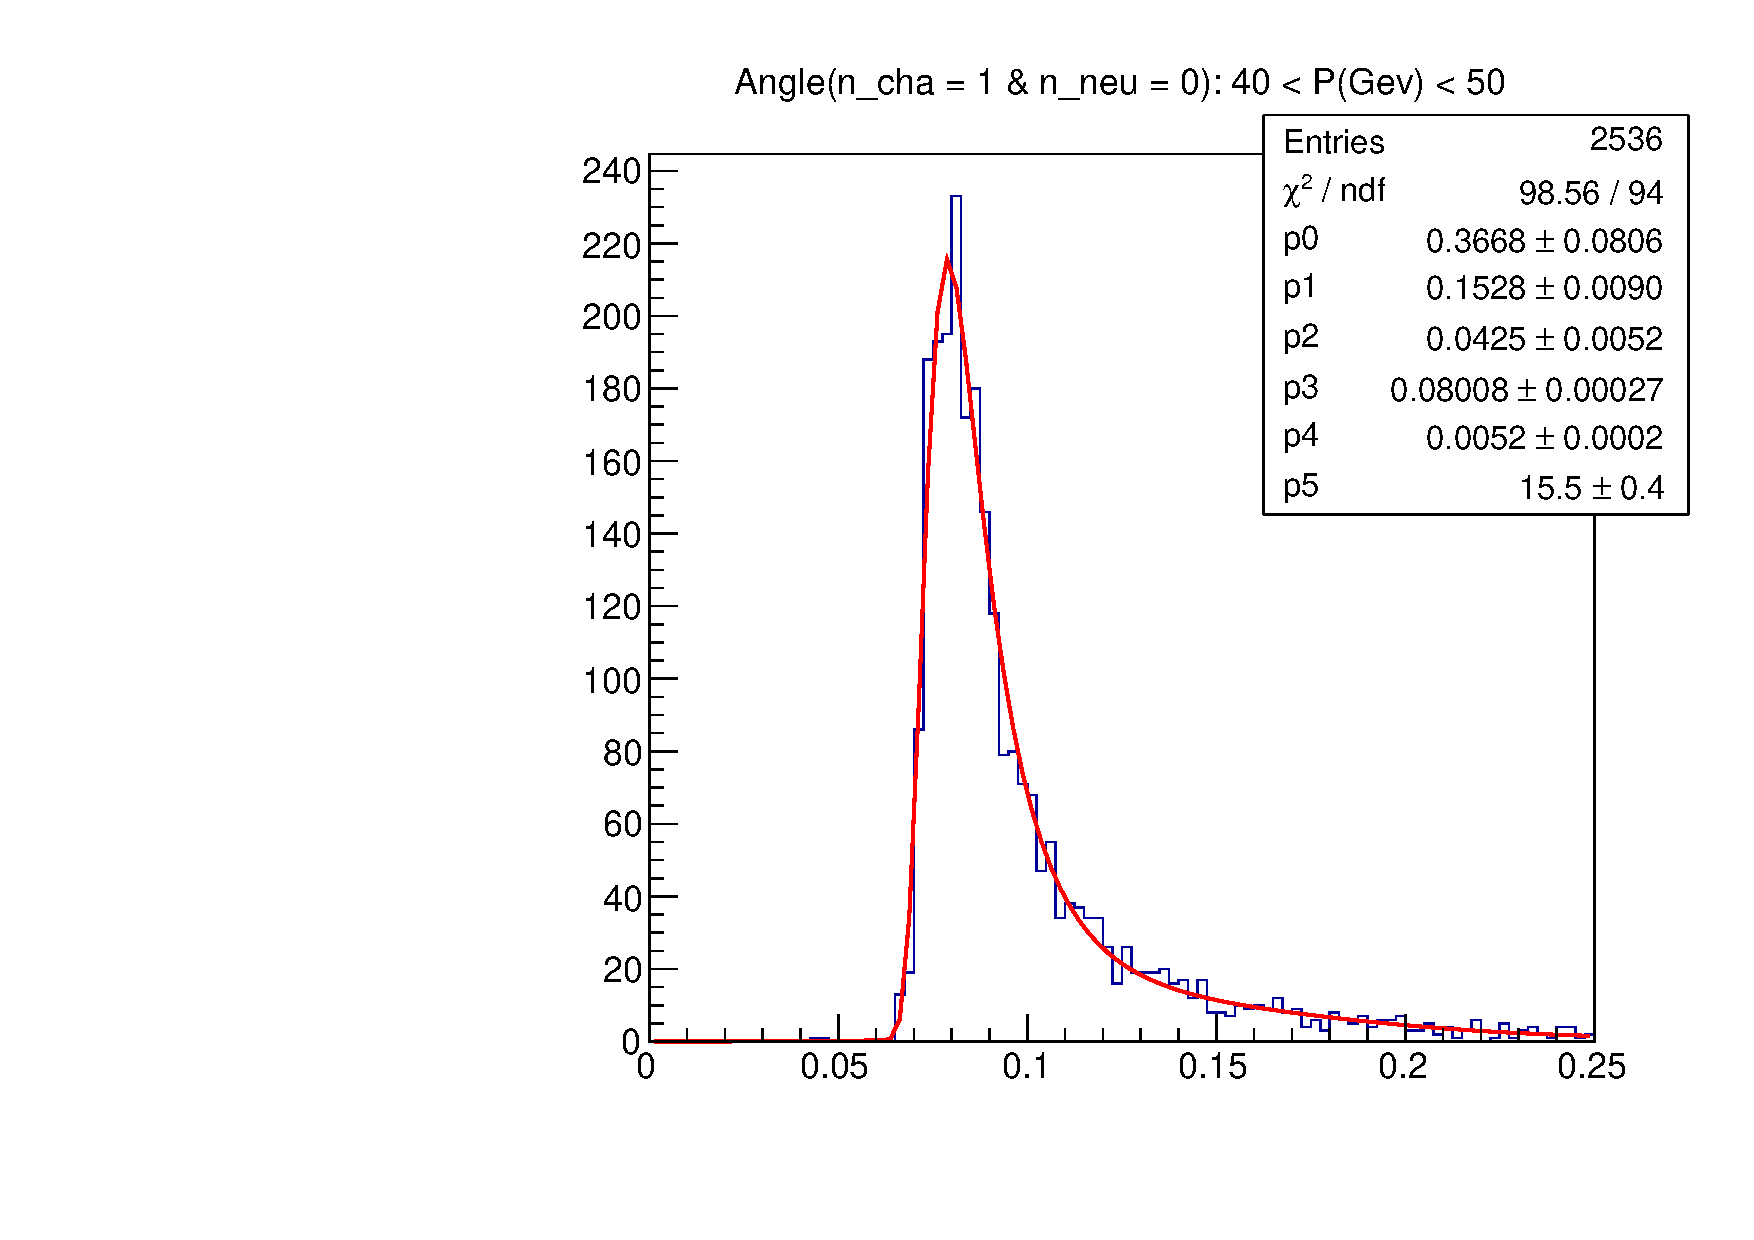
\includegraphics[width=.50\textwidth,height=.50\textheight,type=png,ext=.pdf,read=.pdf]{/afs/cern.ch/work/a/atpathak/public/Pixel/LFV_Plots/Plots_Fit_tautau/Angle_Vis_neutrino_decay1_Fit_2}
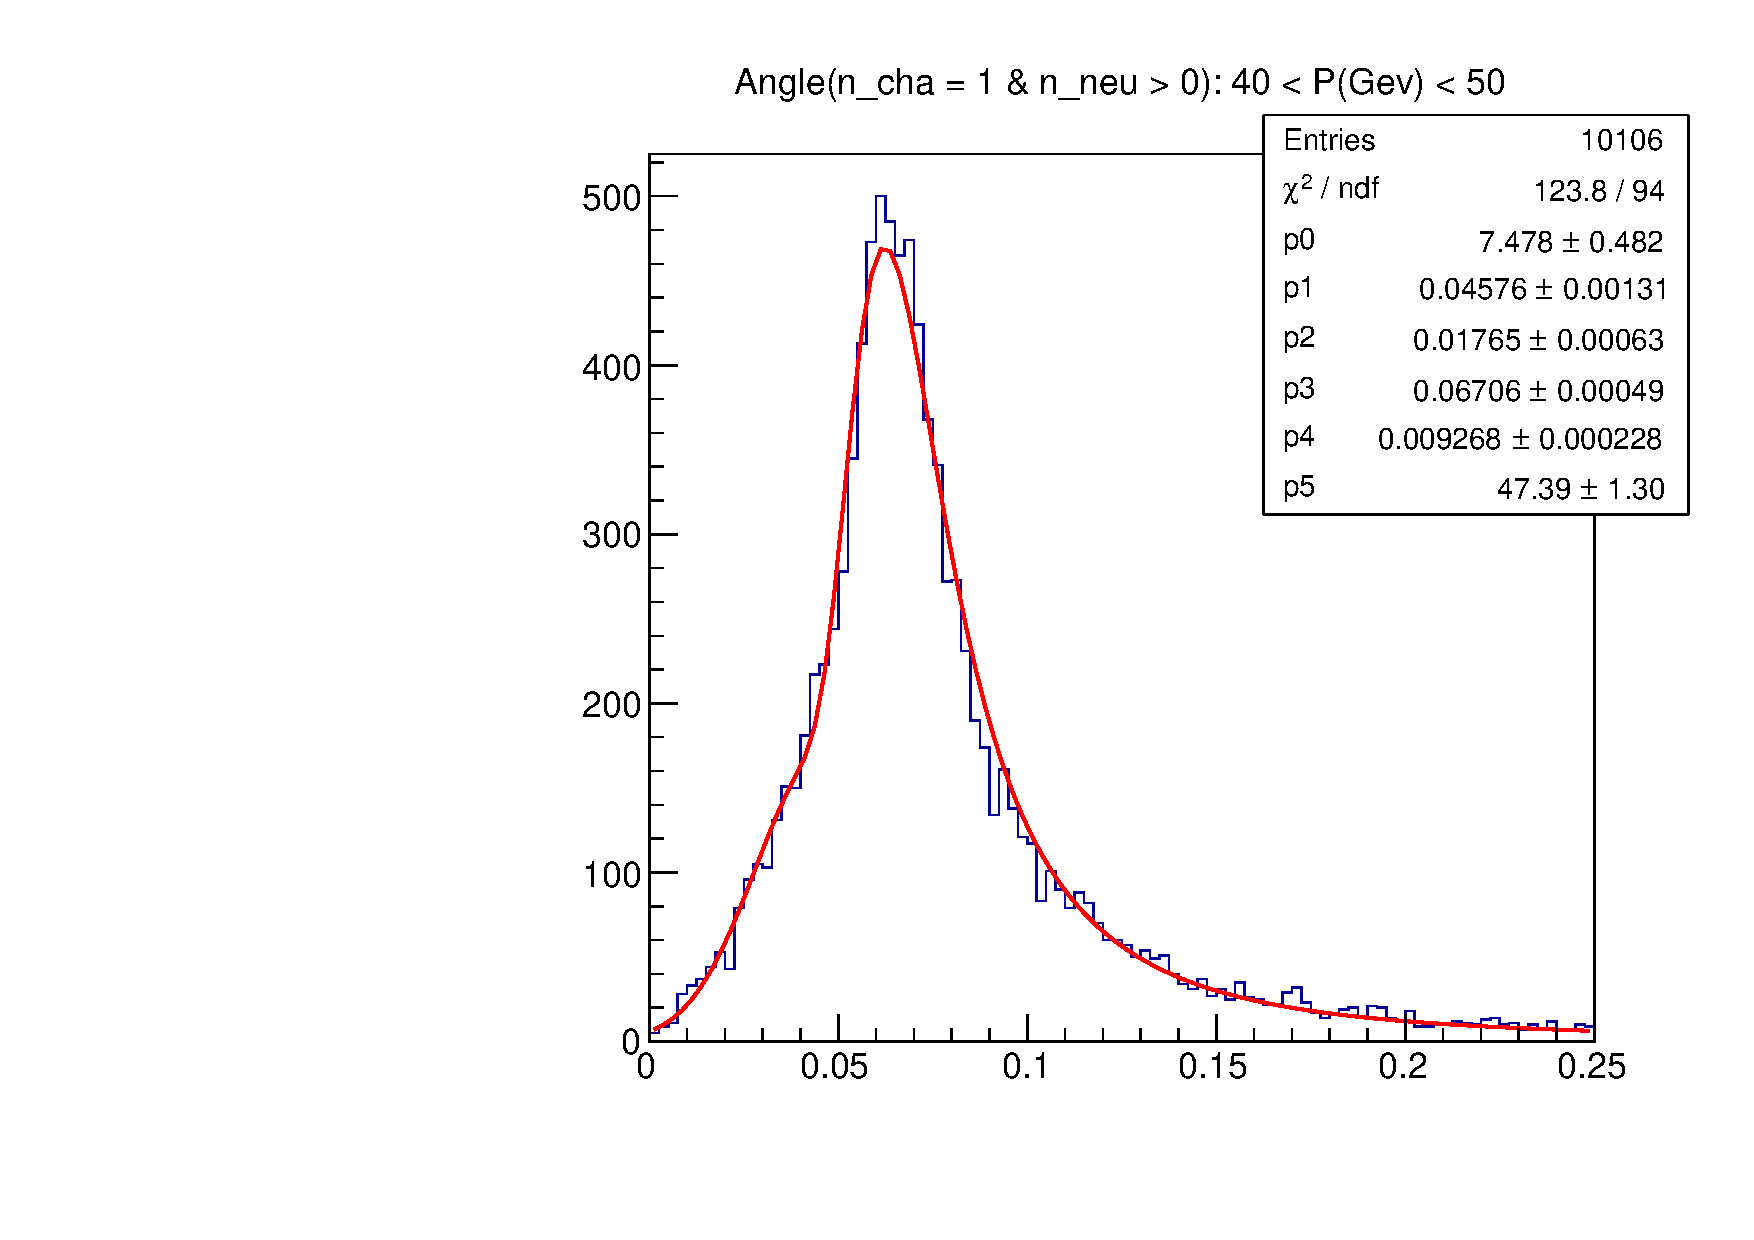
\includegraphics[width=.50\textwidth,height=.50\textheight,type=png,ext=.pdf,read=.pdf]{/afs/cern.ch/work/a/atpathak/public/Pixel/LFV_Plots/Plots_Fit_tautau/Angle_Vis_neutrino_decay2_Fit_2}\\
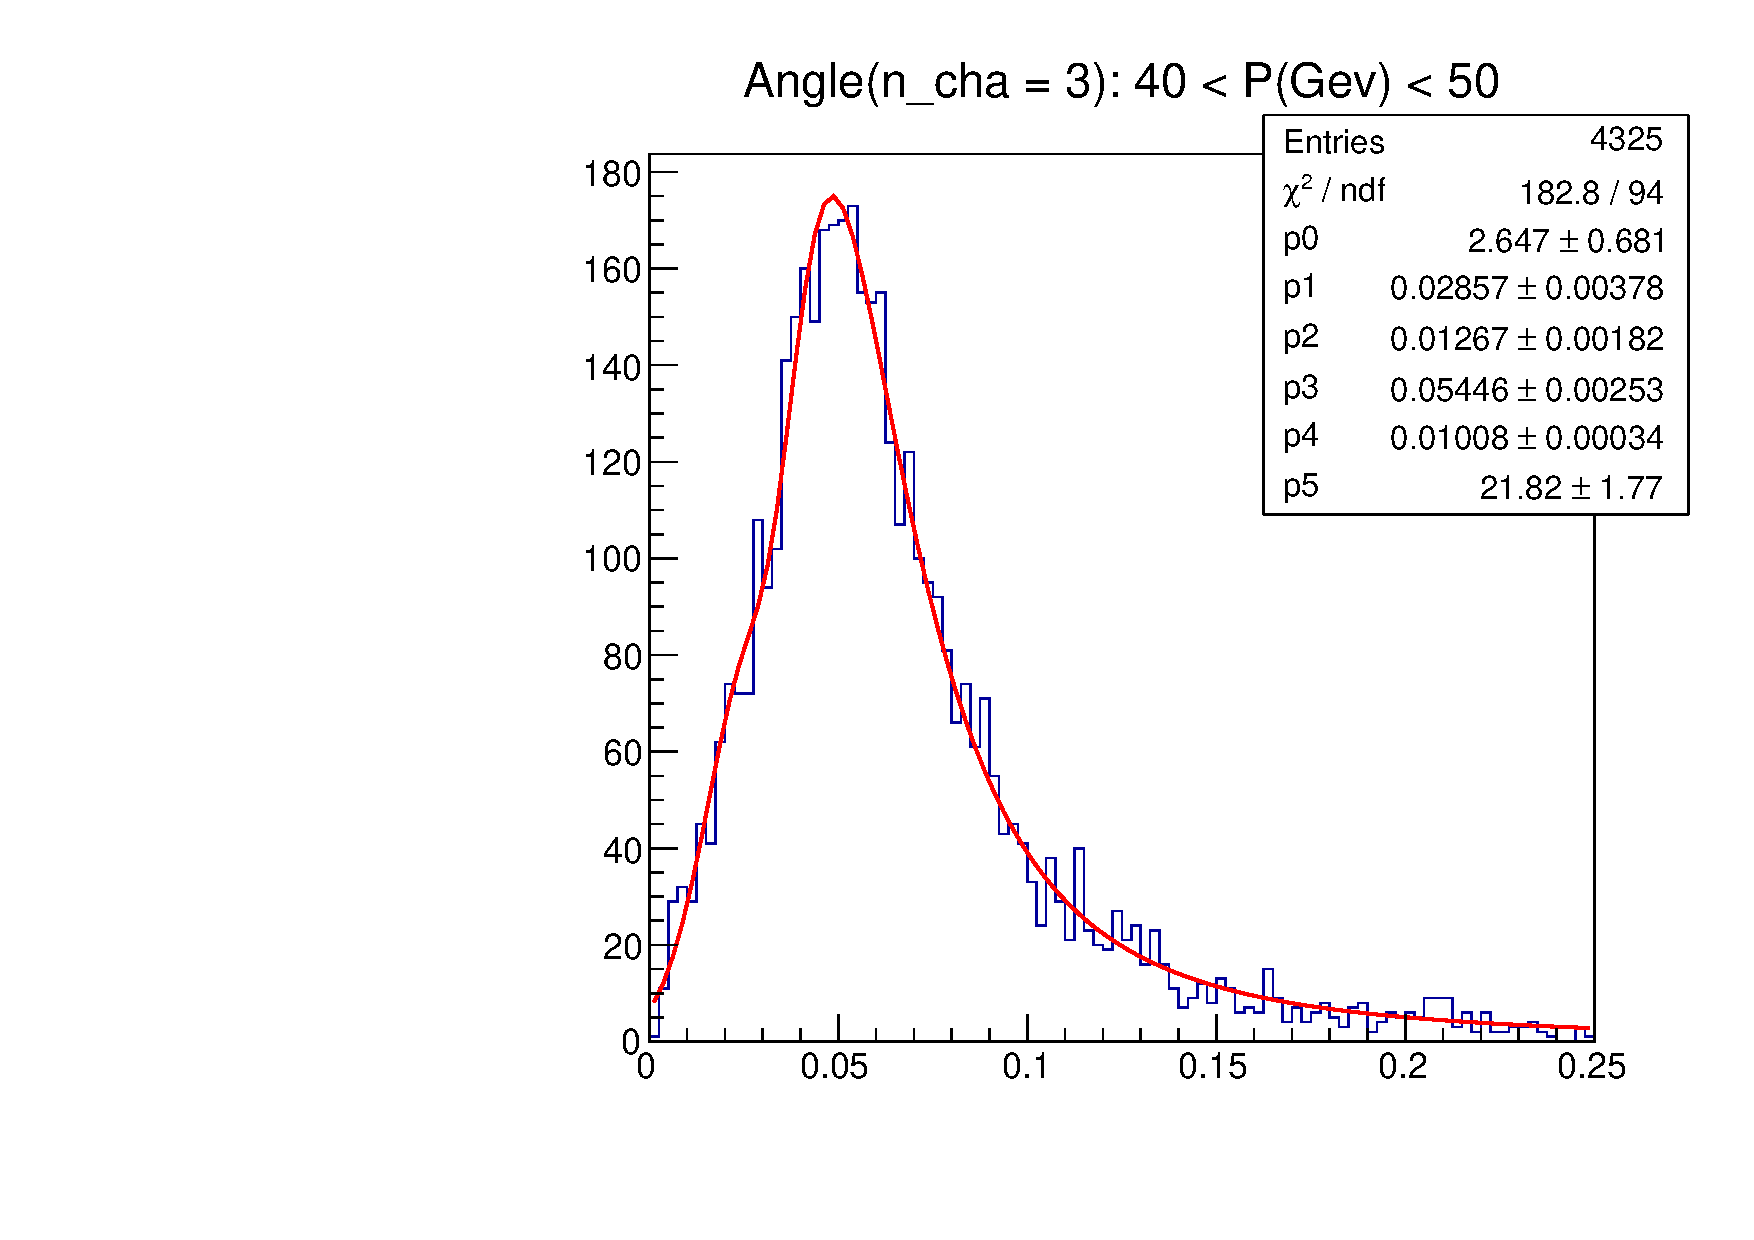
\includegraphics[width=.45\textwidth,height=.45\textheight,type=png,ext=.pdf,read=.pdf]{/afs/cern.ch/work/a/atpathak/public/Pixel/LFV_Plots/Plots_Fit_tautau/Angle_Vis_neutrino_decay3_Fit_2}   
\end{center}
\end{normalsize}

\end {frame}
%------------------------------------------------
\begin{frame}

\begin{normalsize}
\begin{center}
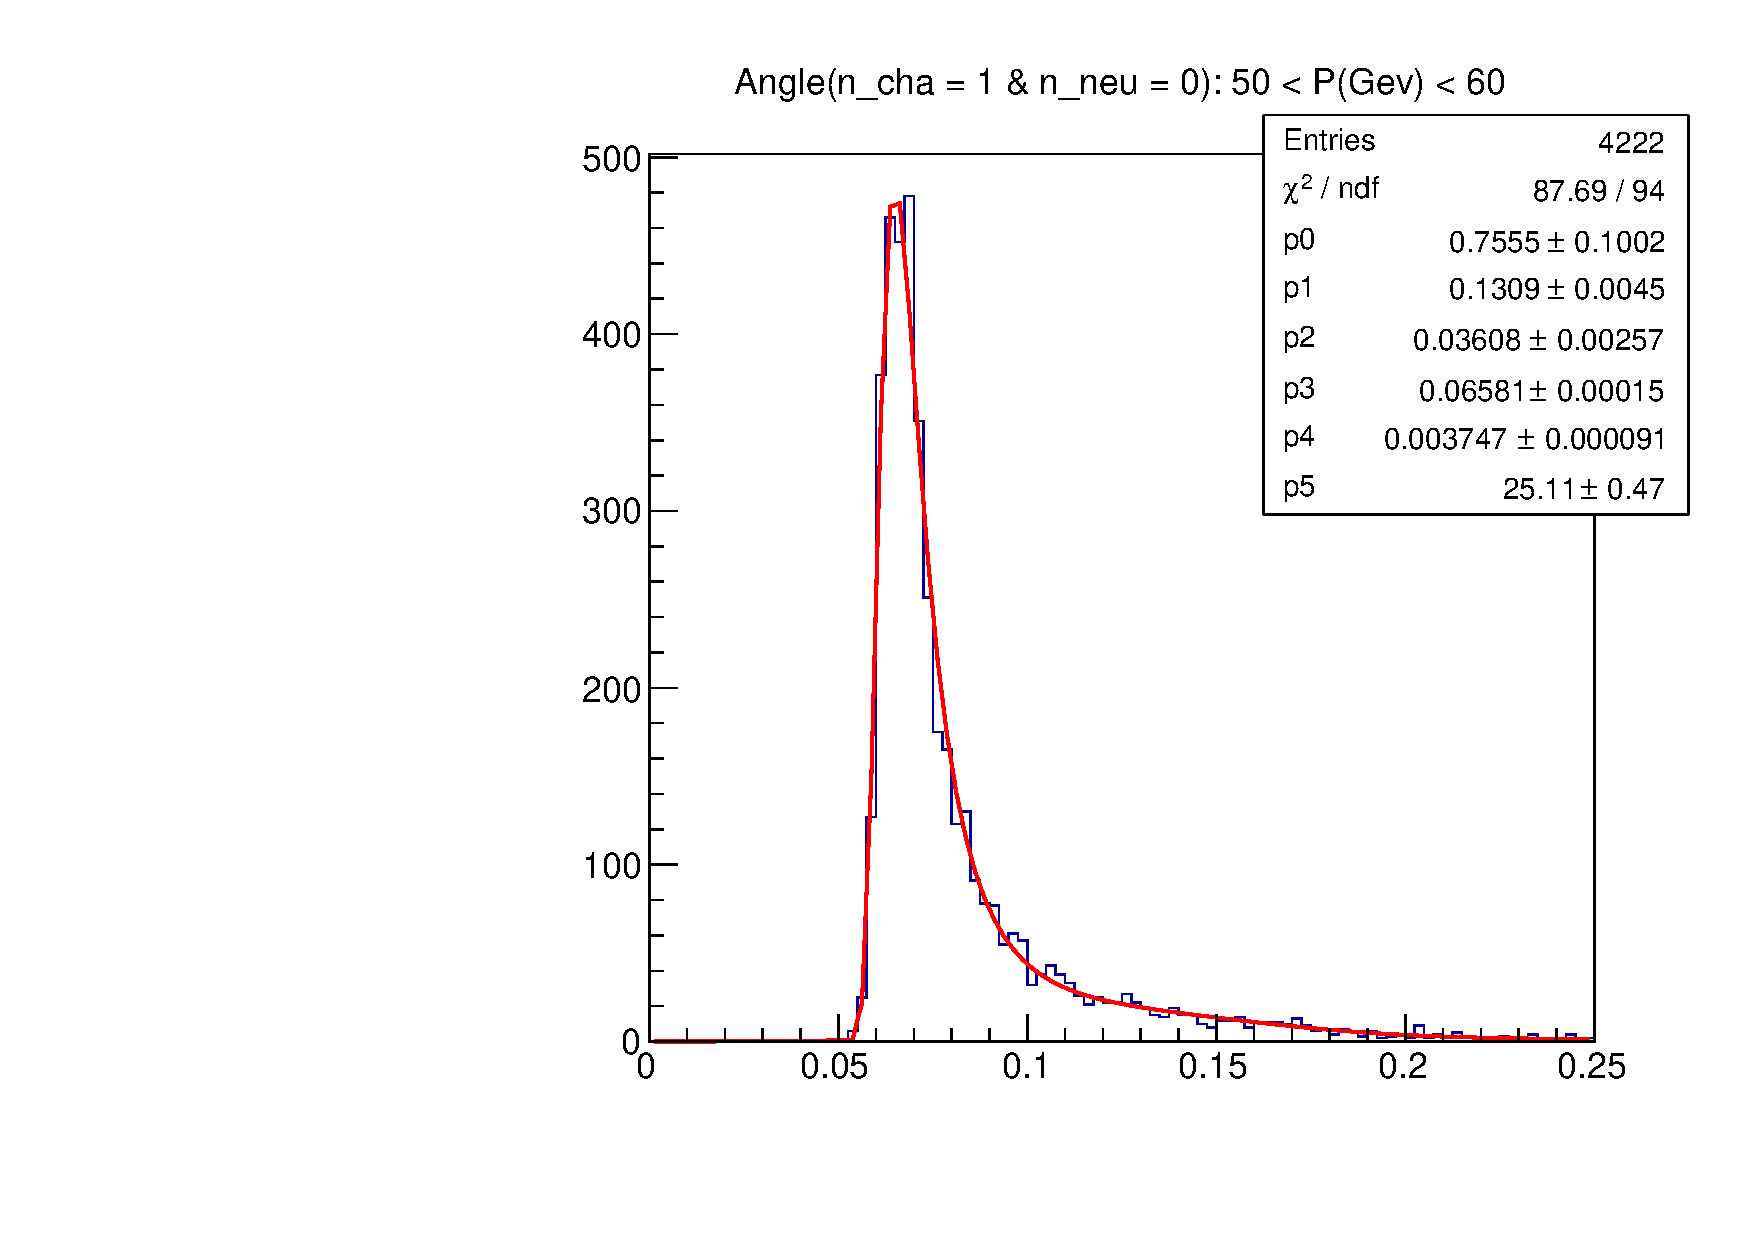
\includegraphics[width=.50\textwidth,height=.50\textheight,type=png,ext=.pdf,read=.pdf]{/afs/cern.ch/work/a/atpathak/public/Pixel/LFV_Plots/Plots_Fit_tautau/Angle_Vis_neutrino_decay1_Fit_3}
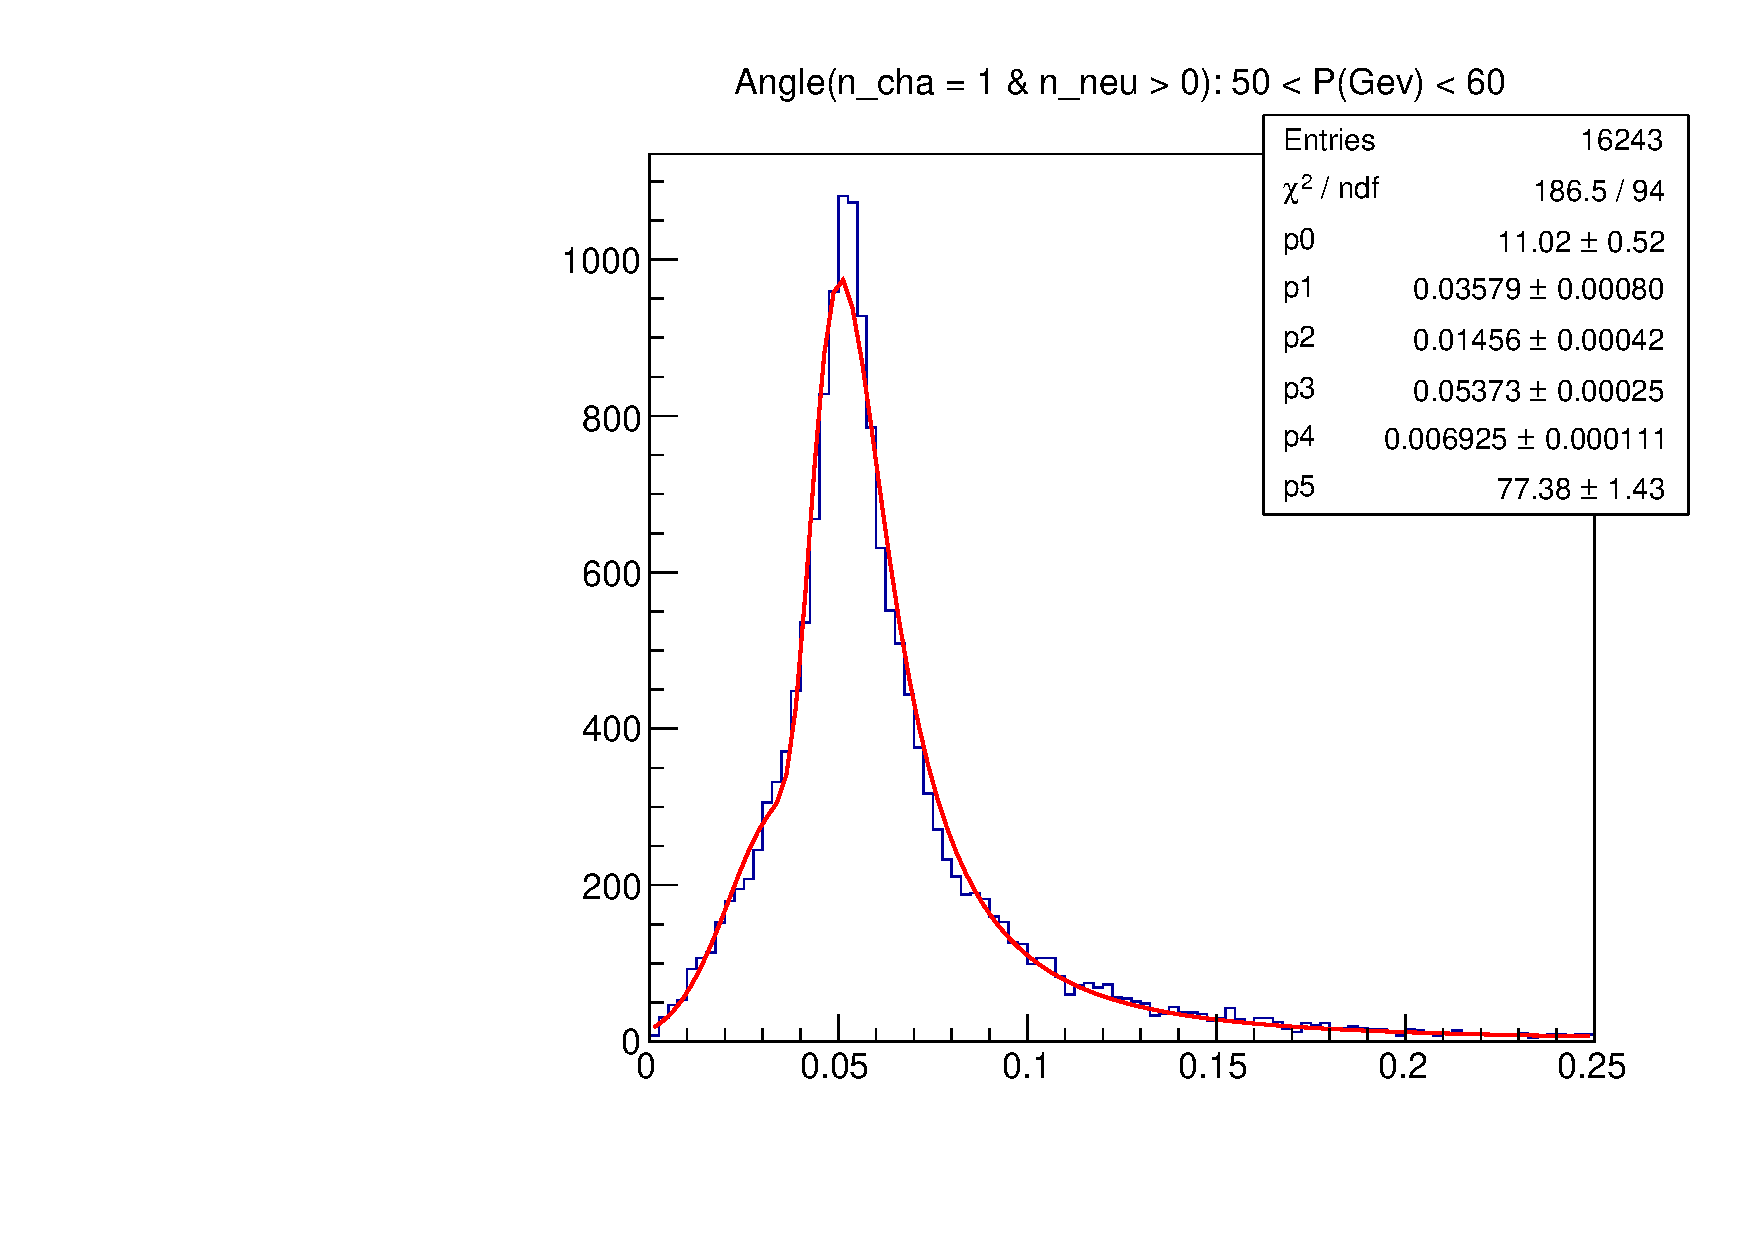
\includegraphics[width=.50\textwidth,height=.50\textheight,type=png,ext=.pdf,read=.pdf]{/afs/cern.ch/work/a/atpathak/public/Pixel/LFV_Plots/Plots_Fit_tautau/Angle_Vis_neutrino_decay2_Fit_3}\\
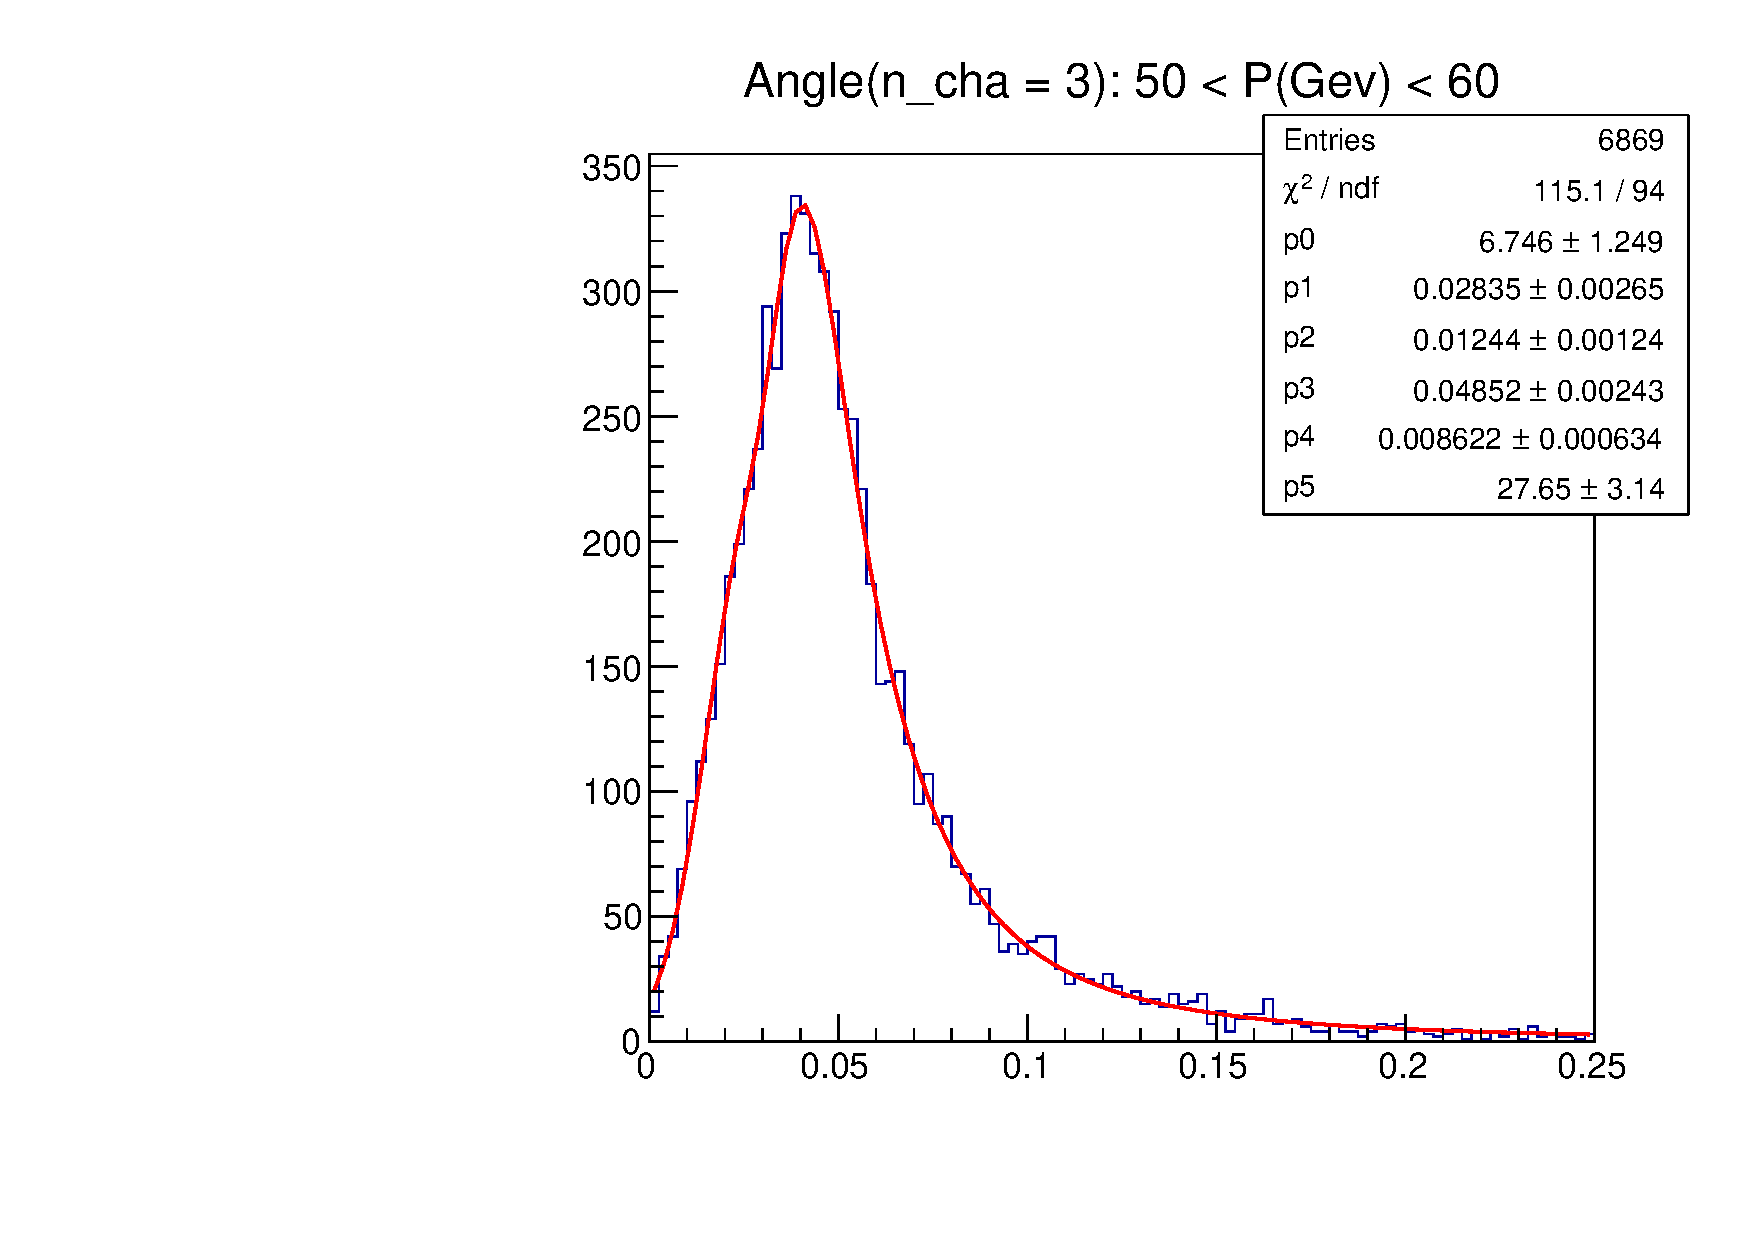
\includegraphics[width=.45\textwidth,height=.45\textheight,type=png,ext=.pdf,read=.pdf]{/afs/cern.ch/work/a/atpathak/public/Pixel/LFV_Plots/Plots_Fit_tautau/Angle_Vis_neutrino_decay3_Fit_3} 
\end{center}
\end{normalsize}

\end {frame}
%------------------------------------------------
\begin{frame}

\begin{normalsize}
\begin{center}
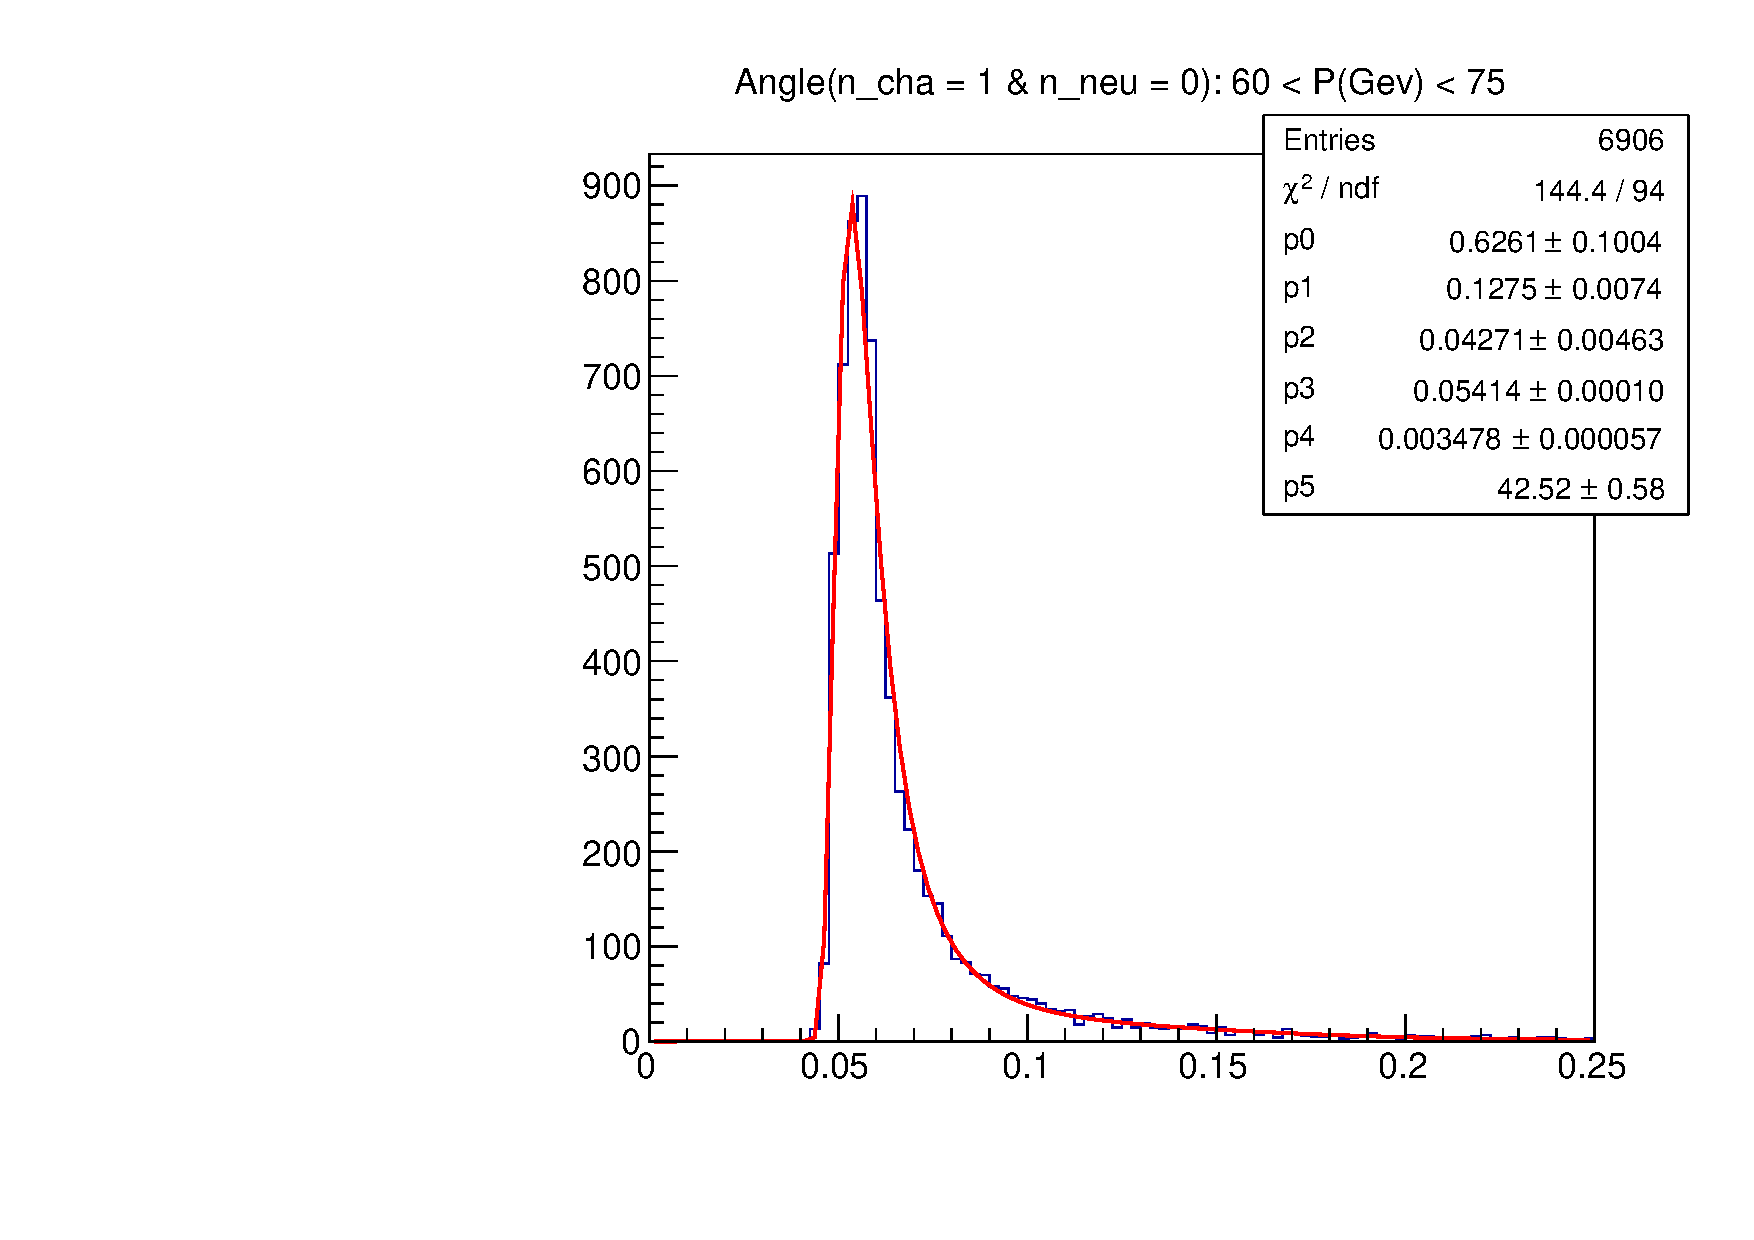
\includegraphics[width=.50\textwidth,height=.50\textheight,type=png,ext=.pdf,read=.pdf]{/afs/cern.ch/work/a/atpathak/public/Pixel/LFV_Plots/Plots_Fit_tautau/Angle_Vis_neutrino_decay1_Fit_4}
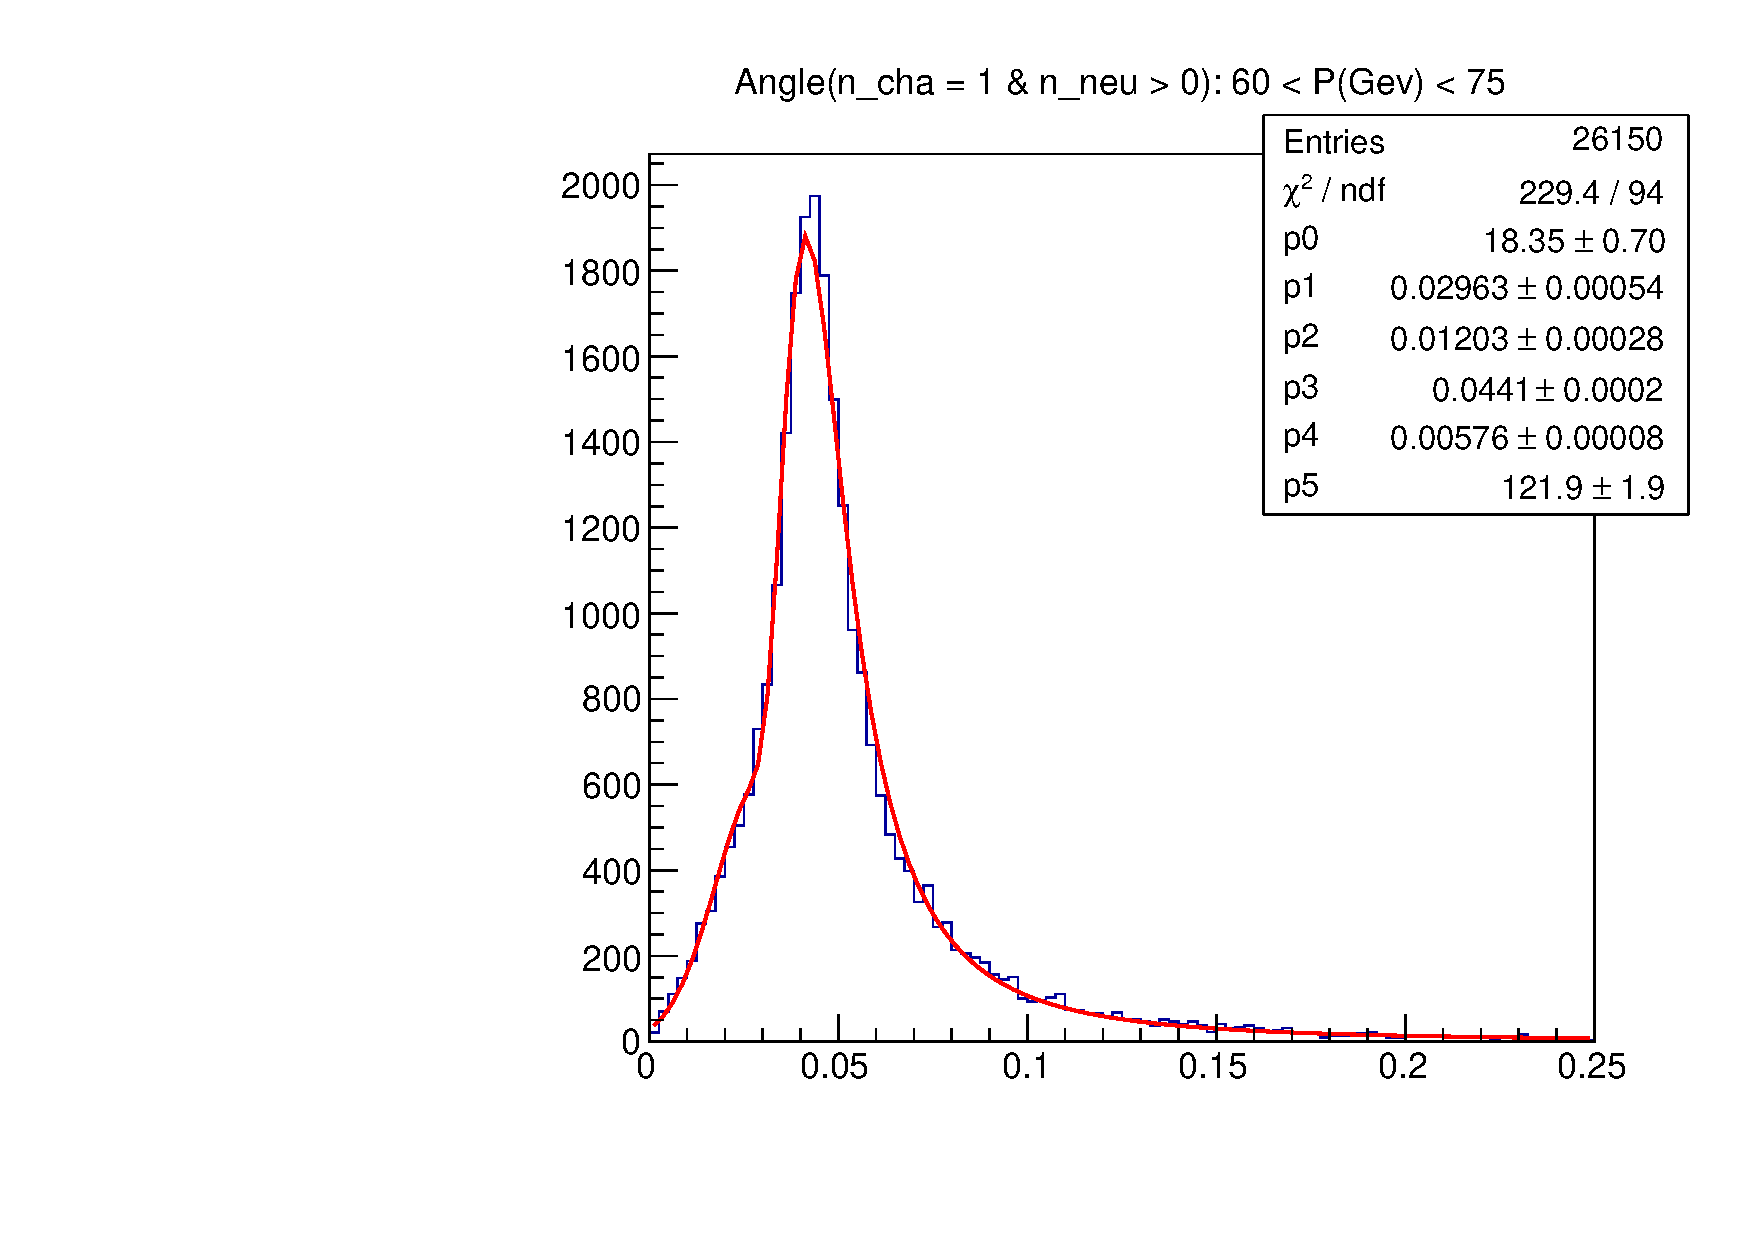
\includegraphics[width=.50\textwidth,height=.50\textheight,type=png,ext=.pdf,read=.pdf]{/afs/cern.ch/work/a/atpathak/public/Pixel/LFV_Plots/Plots_Fit_tautau/Angle_Vis_neutrino_decay2_Fit_4}\\
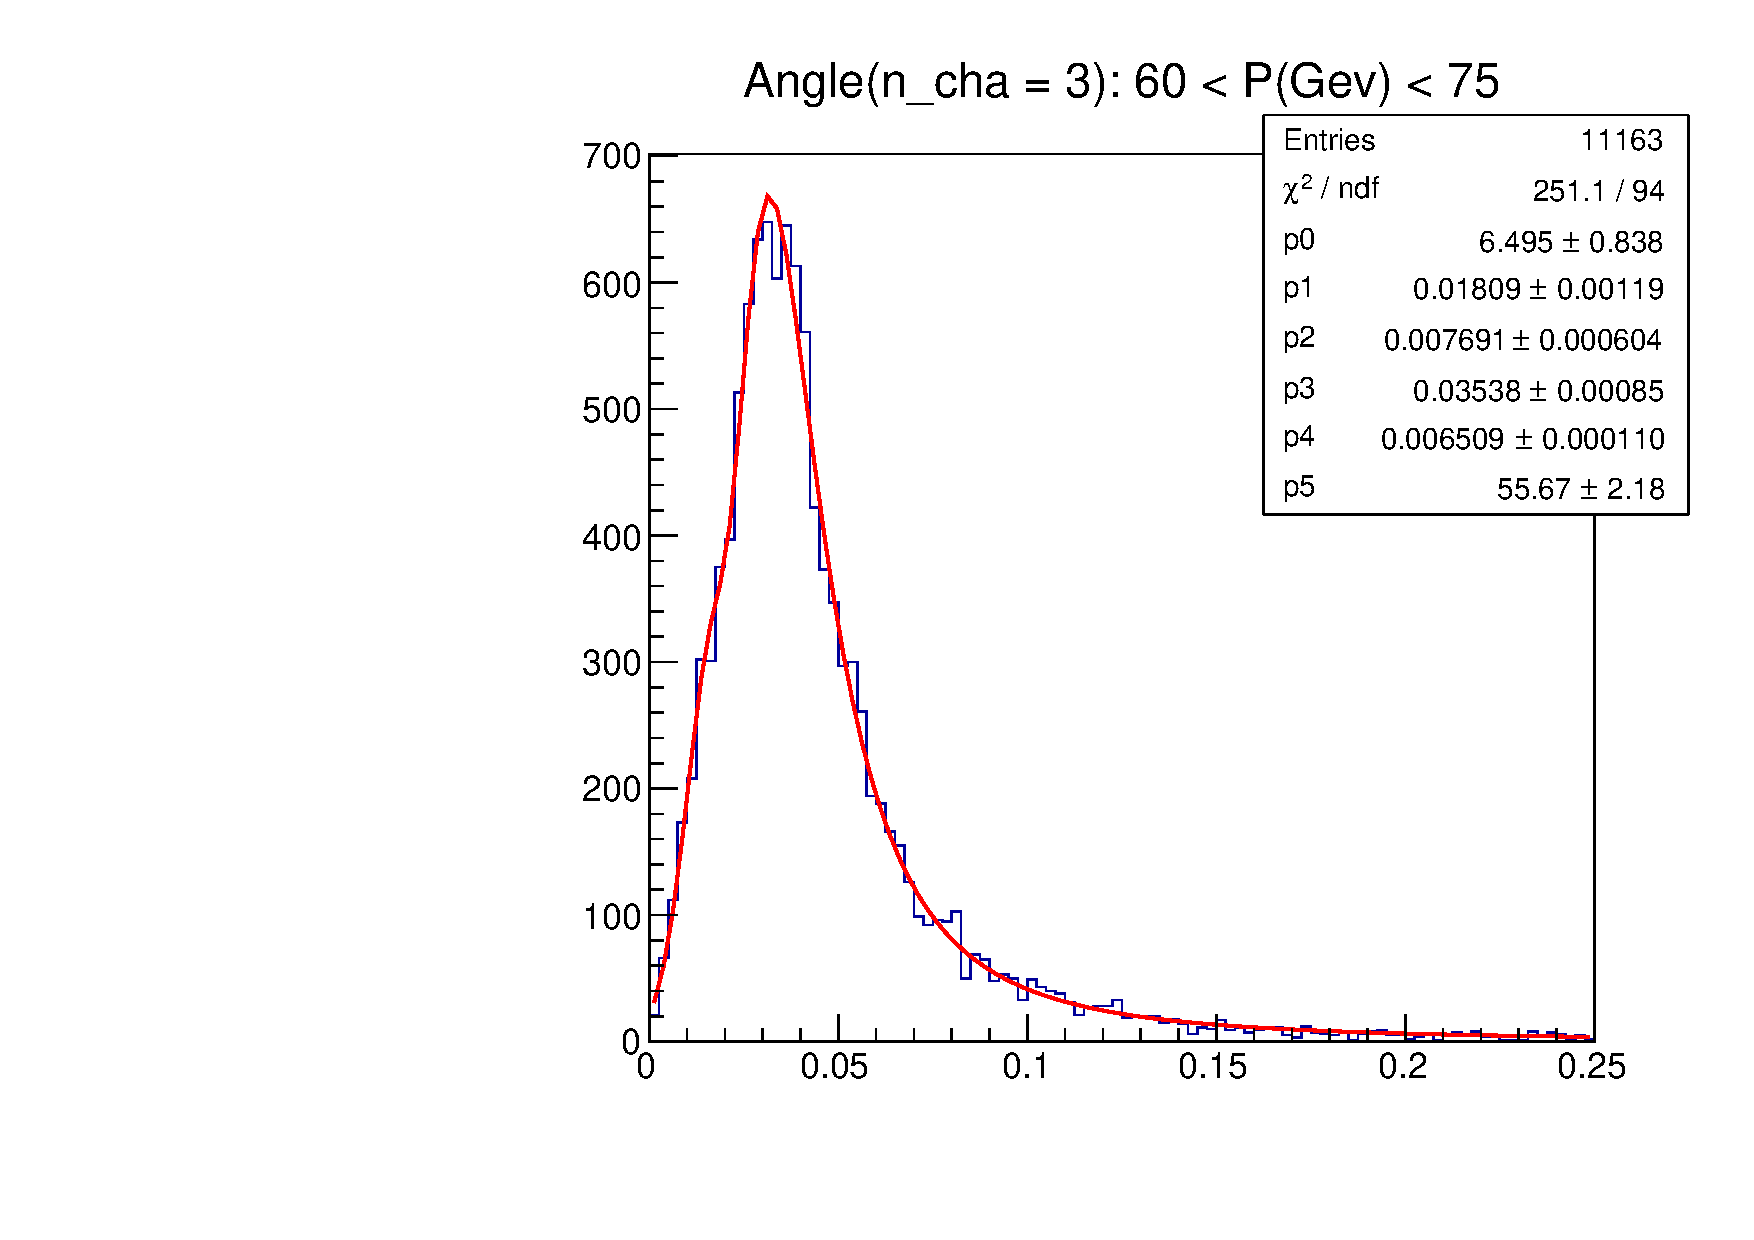
\includegraphics[width=.45\textwidth,height=.45\textheight,type=png,ext=.pdf,read=.pdf]{/afs/cern.ch/work/a/atpathak/public/Pixel/LFV_Plots/Plots_Fit_tautau/Angle_Vis_neutrino_decay3_Fit_4} 
\end{center}
\end{normalsize}

\end {frame}
%------------------------------------------------
\begin{frame}

\begin{normalsize}
\begin{center}
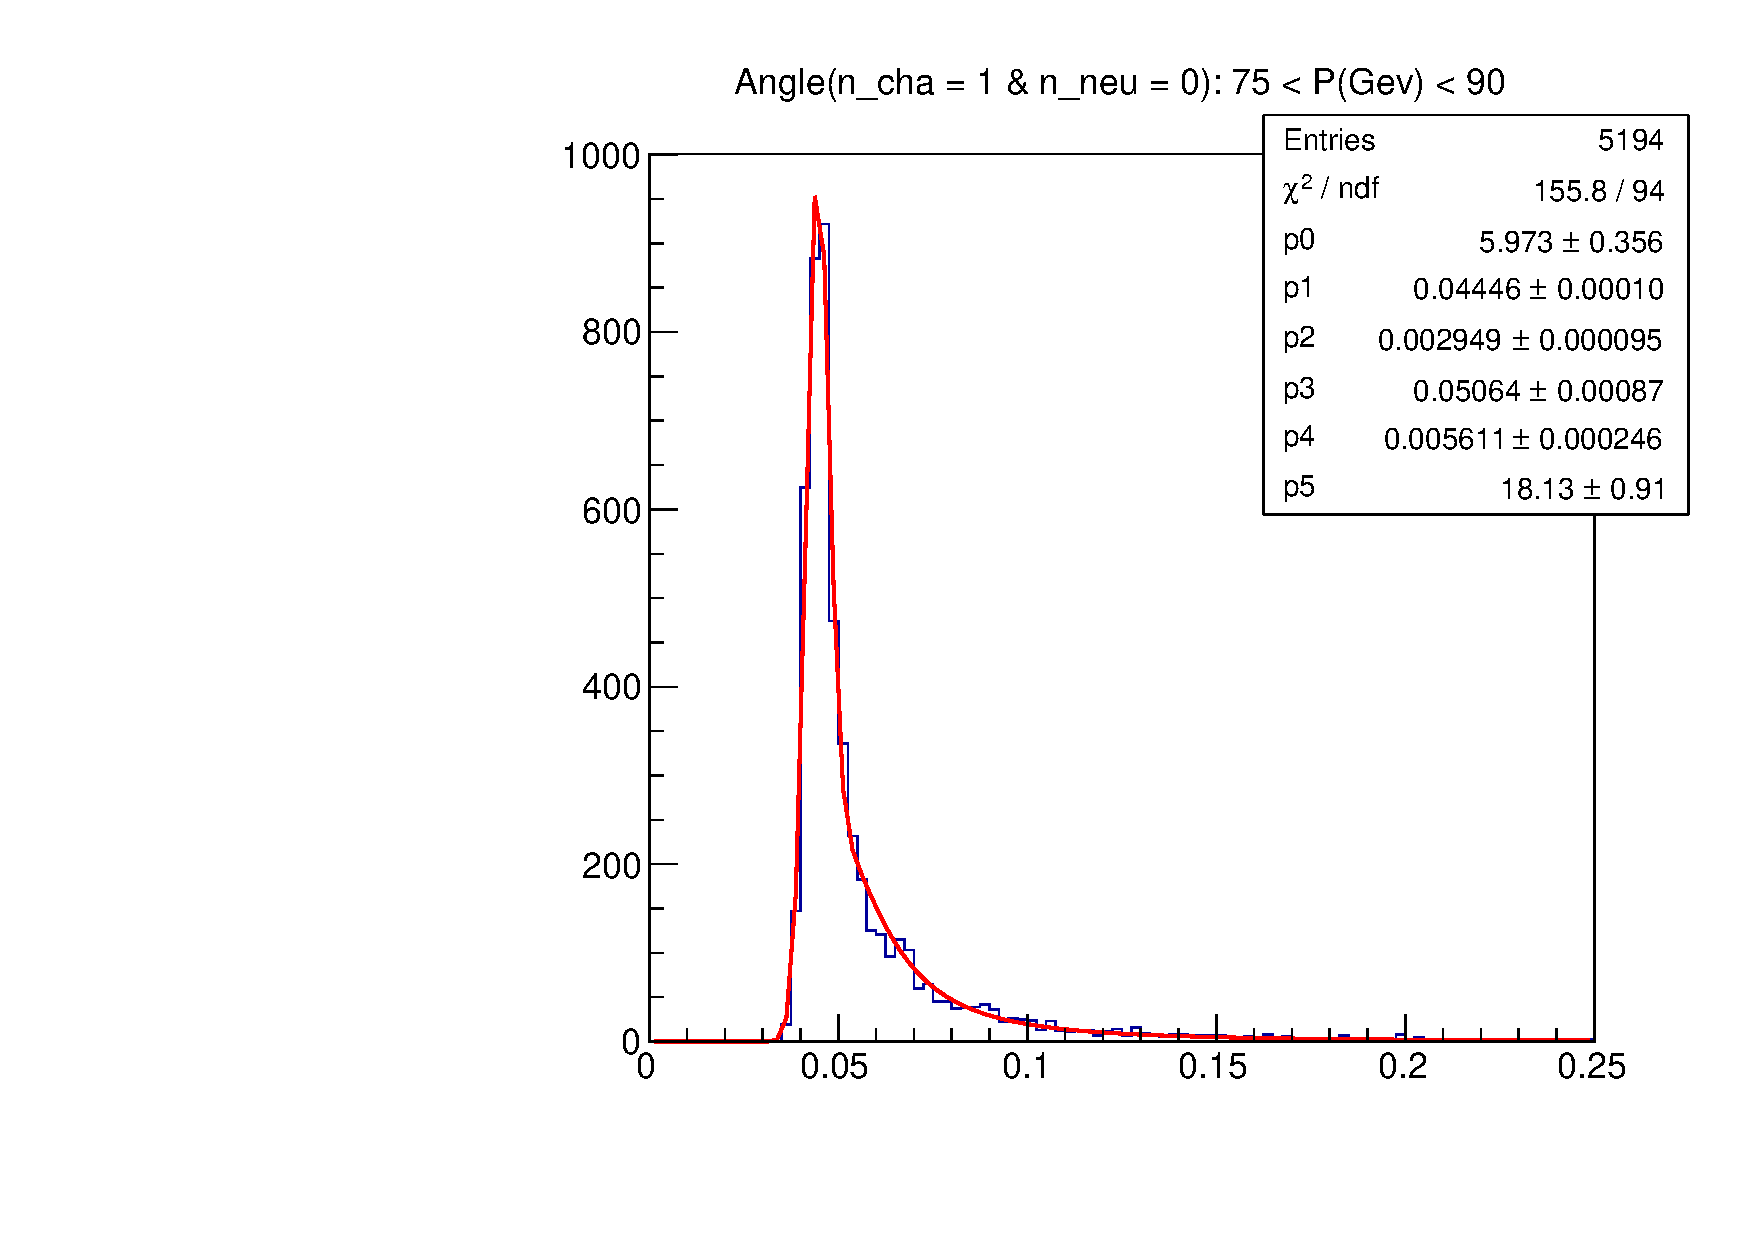
\includegraphics[width=.50\textwidth,height=.50\textheight,type=png,ext=.pdf,read=.pdf]{/afs/cern.ch/work/a/atpathak/public/Pixel/LFV_Plots/Plots_Fit_tautau/Angle_Vis_neutrino_decay1_Fit_5}
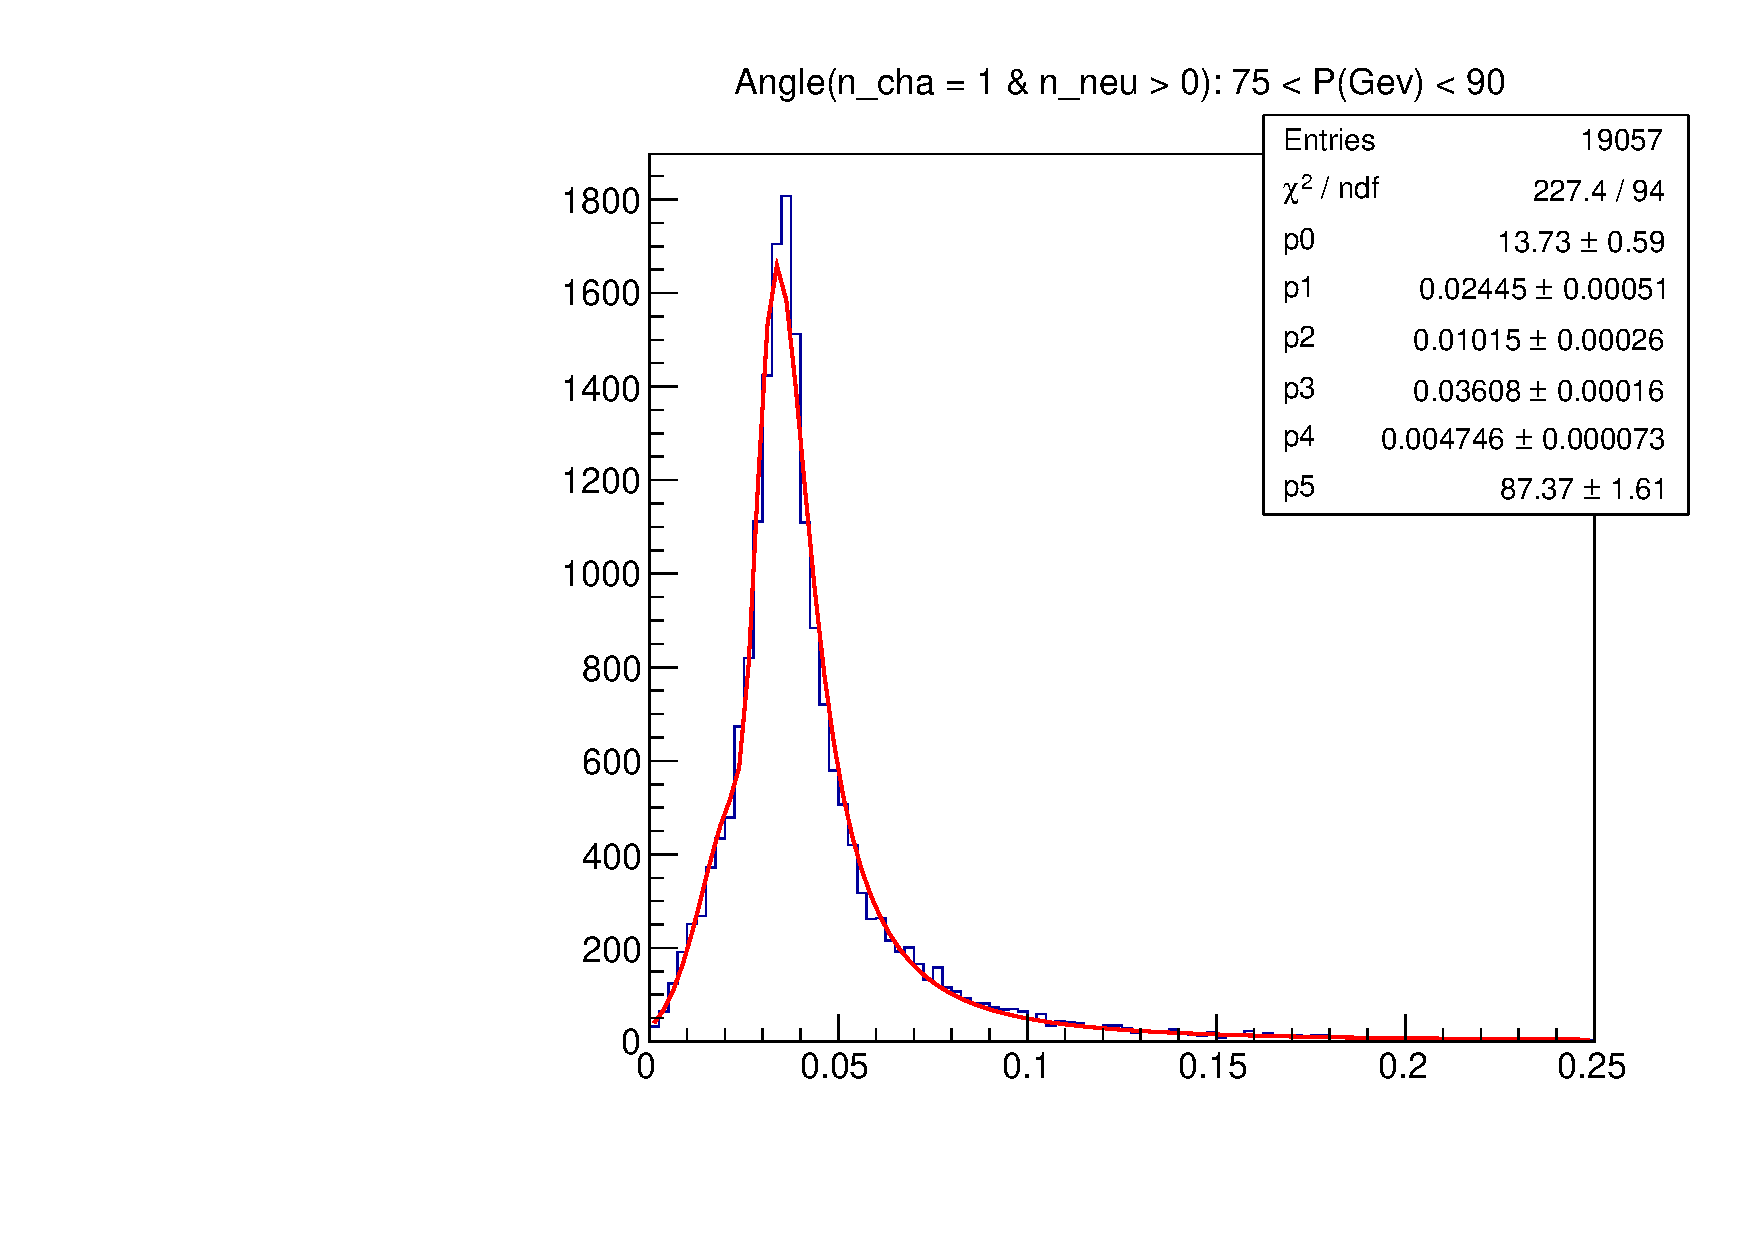
\includegraphics[width=.50\textwidth,height=.50\textheight,type=png,ext=.pdf,read=.pdf]{/afs/cern.ch/work/a/atpathak/public/Pixel/LFV_Plots/Plots_Fit_tautau/Angle_Vis_neutrino_decay2_Fit_5}\\
\includegraphics[width=.45\textwidth,height=.45\textheight,type=png,ext=.pdf,read=.pdf]{/afs/cern.ch/work/a/atpathak/public/Pixel/LFV_Plots/Plots_Fit_tautau/Angle_Vis_neutrino_decay3_Fit_5}  
\end{center}
\end{normalsize}

\end {frame}
%------------------------------------------------
\begin{frame}

\begin{normalsize}
\begin{center}
\includegraphics[width=.50\textwidth,height=.50\textheight,type=png,ext=.pdf,read=.pdf]{/afs/cern.ch/work/a/atpathak/public/Pixel/LFV_Plots/Plots_Fit_tautau/Angle_Vis_neutrino_decay1_Fit_6}
\includegraphics[width=.50\textwidth,height=.50\textheight,type=png,ext=.pdf,read=.pdf]{/afs/cern.ch/work/a/atpathak/public/Pixel/LFV_Plots/Plots_Fit_tautau/Angle_Vis_neutrino_decay2_Fit_6}\\
\includegraphics[width=.45\textwidth,height=.45\textheight,type=png,ext=.pdf,read=.pdf]{/afs/cern.ch/work/a/atpathak/public/Pixel/LFV_Plots/Plots_Fit_tautau/Angle_Vis_neutrino_decay3_Fit_6}   
\end{center}
\end{normalsize}

\end {frame}
%------------------------------------------------
\begin{frame}

\begin{normalsize}
\begin{center}
\includegraphics[width=.50\textwidth,height=.50\textheight,type=png,ext=.pdf,read=.pdf]{/afs/cern.ch/work/a/atpathak/public/Pixel/LFV_Plots/Plots_Fit_tautau/Angle_Vis_neutrino_decay1_Fit_7}
\includegraphics[width=.50\textwidth,height=.50\textheight,type=png,ext=.pdf,read=.pdf]{/afs/cern.ch/work/a/atpathak/public/Pixel/LFV_Plots/Plots_Fit_tautau/Angle_Vis_neutrino_decay2_Fit_7}\\
\includegraphics[width=.45\textwidth,height=.45\textheight,type=png,ext=.pdf,read=.pdf]{/afs/cern.ch/work/a/atpathak/public/Pixel/LFV_Plots/Plots_Fit_tautau/Angle_Vis_neutrino_decay3_Fit_7}  
\end{center}
\end{normalsize}

\end {frame}
%------------------------------------------------
\begin{frame}

\begin{normalsize}
\begin{center}
\includegraphics[width=.50\textwidth,height=.50\textheight,type=png,ext=.pdf,read=.pdf]{/afs/cern.ch/work/a/atpathak/public/Pixel/LFV_Plots/Plots_Fit_tautau/Angle_Vis_neutrino_decay1_Fit_8}
\includegraphics[width=.50\textwidth,height=.50\textheight,type=png,ext=.pdf,read=.pdf]{/afs/cern.ch/work/a/atpathak/public/Pixel/LFV_Plots/Plots_Fit_tautau/Angle_Vis_neutrino_decay2_Fit_8}\\
\includegraphics[width=.45\textwidth,height=.45\textheight,type=png,ext=.pdf,read=.pdf]{/afs/cern.ch/work/a/atpathak/public/Pixel/LFV_Plots/Plots_Fit_tautau/Angle_Vis_neutrino_decay3_Fit_8} 
\end{center}
\end{normalsize}

\end {frame}
%------------------------------------------------
\begin{frame}

\begin{normalsize}
\begin{center}
\includegraphics[width=.50\textwidth,height=.50\textheight,type=png,ext=.pdf,read=.pdf]{/afs/cern.ch/work/a/atpathak/public/Pixel/LFV_Plots/Plots_Fit_tautau/Angle_Vis_neutrino_decay1_Fit_9}
\includegraphics[width=.50\textwidth,height=.50\textheight,type=png,ext=.pdf,read=.pdf]{/afs/cern.ch/work/a/atpathak/public/Pixel/LFV_Plots/Plots_Fit_tautau/Angle_Vis_neutrino_decay2_Fit_9}\\
\includegraphics[width=.45\textwidth,height=.45\textheight,type=png,ext=.pdf,read=.pdf]{/afs/cern.ch/work/a/atpathak/public/Pixel/LFV_Plots/Plots_Fit_tautau/Angle_Vis_neutrino_decay3_Fit_9} 
\end{center}
\end{normalsize}

\end {frame}
%------------------------------------------------
\begin{frame}

\begin{normalsize}
\begin{center}
\includegraphics[width=.50\textwidth,height=.50\textheight,type=png,ext=.pdf,read=.pdf]{/afs/cern.ch/work/a/atpathak/public/Pixel/LFV_Plots/Plots_Fit_tautau/Angle_Vis_neutrino_decay1_Fit_10}
\includegraphics[width=.50\textwidth,height=.50\textheight,type=png,ext=.pdf,read=.pdf]{/afs/cern.ch/work/a/atpathak/public/Pixel/LFV_Plots/Plots_Fit_tautau/Angle_Vis_neutrino_decay2_Fit_10}\\
\includegraphics[width=.45\textwidth,height=.45\textheight,type=png,ext=.pdf,read=.pdf]{/afs/cern.ch/work/a/atpathak/public/Pixel/LFV_Plots/Plots_Fit_tautau/Angle_Vis_neutrino_decay3_Fit_10} 
\end{center}
\end{normalsize}

\end {frame}
%------------------------------------------------
\begin{frame}

\begin{normalsize}
\begin{center}
\includegraphics[width=.50\textwidth,height=.50\textheight,type=png,ext=.pdf,read=.pdf]{/afs/cern.ch/work/a/atpathak/public/Pixel/LFV_Plots/Plots_Fit_tautau/decay0_FitP0}
\includegraphics[width=.50\textwidth,height=.50\textheight,type=png,ext=.pdf,read=.pdf]{/afs/cern.ch/work/a/atpathak/public/Pixel/LFV_Plots/Plots_Fit_tautau/decay1_FitP0}\\
\includegraphics[width=.45\textwidth,height=.45\textheight,type=png,ext=.pdf,read=.pdf]{/afs/cern.ch/work/a/atpathak/public/Pixel/LFV_Plots/Plots_Fit_tautau/decay2_FitP0}  
\end{center}
\end{normalsize}

\end {frame}
%------------------------------------------------
\begin{frame}

\begin{normalsize}
\begin{center}
\includegraphics[width=.50\textwidth,height=.50\textheight,type=png,ext=.pdf,read=.pdf]{/afs/cern.ch/work/a/atpathak/public/Pixel/LFV_Plots/Plots_Fit_tautau/decay0_FitP1}
\includegraphics[width=.50\textwidth,height=.50\textheight,type=png,ext=.pdf,read=.pdf]{/afs/cern.ch/work/a/atpathak/public/Pixel/LFV_Plots/Plots_Fit_tautau/decay1_FitP1}\\
\includegraphics[width=.45\textwidth,height=.45\textheight,type=png,ext=.pdf,read=.pdf]{/afs/cern.ch/work/a/atpathak/public/Pixel/LFV_Plots/Plots_Fit_tautau/decay2_FitP1}  
\end{center}
\end{normalsize}

\end {frame}
%------------------------------------------------
\begin{frame}

\begin{normalsize}
\begin{center}
\includegraphics[width=.50\textwidth,height=.50\textheight,type=png,ext=.pdf,read=.pdf]{/afs/cern.ch/work/a/atpathak/public/Pixel/LFV_Plots/Plots_Fit_tautau/decay0_FitP2}
\includegraphics[width=.50\textwidth,height=.50\textheight,type=png,ext=.pdf,read=.pdf]{/afs/cern.ch/work/a/atpathak/public/Pixel/LFV_Plots/Plots_Fit_tautau/decay1_FitP2}\\
\includegraphics[width=.45\textwidth,height=.45\textheight,type=png,ext=.pdf,read=.pdf]{/afs/cern.ch/work/a/atpathak/public/Pixel/LFV_Plots/Plots_Fit_tautau/decay2_FitP2}  
\end{center}
\end{normalsize}

\end {frame}
%------------------------------------------------
\begin{frame}

\begin{normalsize}
\begin{center}
\includegraphics[width=.50\textwidth,height=.50\textheight,type=png,ext=.pdf,read=.pdf]{/afs/cern.ch/work/a/atpathak/public/Pixel/LFV_Plots/Plots_Fit_tautau/decay0_FitP3}
\includegraphics[width=.50\textwidth,height=.50\textheight,type=png,ext=.pdf,read=.pdf]{/afs/cern.ch/work/a/atpathak/public/Pixel/LFV_Plots/Plots_Fit_tautau/decay1_FitP3}\\
\includegraphics[width=.45\textwidth,height=.45\textheight,type=png,ext=.pdf,read=.pdf]{/afs/cern.ch/work/a/atpathak/public/Pixel/LFV_Plots/Plots_Fit_tautau/decay2_FitP3}  
\end{center}
\end{normalsize}

\end {frame}
%------------------------------------------------
\begin{frame}

\begin{normalsize}
\begin{center}
\includegraphics[width=.50\textwidth,height=.50\textheight,type=png,ext=.pdf,read=.pdf]{/afs/cern.ch/work/a/atpathak/public/Pixel/LFV_Plots/Plots_Fit_tautau/decay0_FitP4}
\includegraphics[width=.50\textwidth,height=.50\textheight,type=png,ext=.pdf,read=.pdf]{/afs/cern.ch/work/a/atpathak/public/Pixel/LFV_Plots/Plots_Fit_tautau/decay1_FitP4}\\
\includegraphics[width=.45\textwidth,height=.45\textheight,type=png,ext=.pdf,read=.pdf]{/afs/cern.ch/work/a/atpathak/public/Pixel/LFV_Plots/Plots_Fit_tautau/decay2_FitP4}  
\end{center}
\end{normalsize}

\end {frame}
%------------------------------------------------
\begin{frame}

\begin{normalsize}
\begin{center}
\includegraphics[width=.50\textwidth,height=.50\textheight,type=png,ext=.pdf,read=.pdf]{/afs/cern.ch/work/a/atpathak/public/Pixel/LFV_Plots/Plots_Fit_tautau/decay0_FitP5}
\includegraphics[width=.50\textwidth,height=.50\textheight,type=png,ext=.pdf,read=.pdf]{/afs/cern.ch/work/a/atpathak/public/Pixel/LFV_Plots/Plots_Fit_tautau/decay1_FitP5}\\
\includegraphics[width=.45\textwidth,height=.45\textheight,type=png,ext=.pdf,read=.pdf]{/afs/cern.ch/work/a/atpathak/public/Pixel/LFV_Plots/Plots_Fit_tautau/decay2_FitP5}  
\end{center}
\end{normalsize}

\end {frame}
\fi
\end{document}
%------------------------------------------------
\begin{frame}

\begin{normalsize}
\begin{center}
\includegraphics[width=.44\textwidth,height=.40\textheight,type=png,ext=.pdf,read=.pdf]{/afs/cern.ch/work/a/atpathak/public/ROOTAnalysisTutorial/Plots/Angle_Vis_neutrino_numCharged1_7}
\includegraphics[width=.44\textwidth,height=.40\textheight,type=png,ext=.pdf,read=.pdf]{/afs/cern.ch/work/a/atpathak/public/ROOTAnalysisTutorial/Plots/Angle_Vis_neutrino_numChargedPion1_7}\\
\includegraphics[width=.44\textwidth,height=.40\textheight,type=png,ext=.pdf,read=.pdf]{/afs/cern.ch/work/a/atpathak/public/ROOTAnalysisTutorial/Plots/Angle_Vis_neutrino_numCharged3_7}
\includegraphics[width=.44\textwidth,height=.40\textheight,type=png,ext=.pdf,read=.pdf]{/afs/cern.ch/work/a/atpathak/public/ROOTAnalysisTutorial/Plots/Angle_Vis_neutrino_numChargedPion3_7}
\end{center}
\end{normalsize}

\end {frame}
%------------------------------------------------
\end{document}
%-------------------------------------------------
\begin{frame}
\frametitle{Status of direct search at the LHC}
\begin{changemargin}{-7mm}{0mm}
\textcolor{blue}{\bf Direct search in Run 1}
%\vspace{-1em}
\begin{table}
\begin{center}
{\bf
{\scalebox{.45}{
\renewcommand{\arraystretch}{1.2}
\begin{tabular}{| r | l | c | c | c | c | c | c |}
\hline
\multicolumn{1}{|l|}{H $\to$} & Experiment & \boldmath$ {
                \sqrt{s}}$ (TeV) & \boldmath$ {\int L}$ (fb \boldmath$ {^{-1}}$) & \multicolumn {2}{c|} {Upper
                           Limits at 95\% CL}  & Best Fit Value & Significance \\
\cline{5-6}
& & & & Expected & Observed &(Branching Fraction) & (Observed) \\
\hline
\boldmath$ {\mu\tau}$ & CMS (2012 Data) & 8 & 19.7 & (0.75 \boldmath$ {\pm}$ 0.38)\% & 1.51\%
                            & (0.84 \boldmath$ {^{+0.39}_{-0.37}}$)\% & \textcolor{red}{2.4 \boldmath$ {\sigma}$}\\
&\href{https://arxiv.org/abs/1502.07400}{PLB749 (2015) 337 [1502.07400]} & & & & & & \\
\cline{2-8}
& ATLAS (2012 Data) & 8 & 20.3 &(1.01$\mathbf {^{+0.40}_{-0.29}}$)\%  & 1.43\% &
                              (0.53 $\mathbf {\pm}$ 0.51)\% & \textcolor{red}{1 \boldmath$ {\sigma}$} \\
&\href{https://arxiv.org/abs/1604.07730}{EPJC77 (2017) 70 [1604.07730]} & & & & & & \\
\cline{2-8}
\hline
\boldmath$ { e\tau}$ & CMS (2012 Data) & 8 & 19.7 &(0.75 \boldmath$ {^{+0.32}_{-0.22}}$)\% & 0.69\% &
                               (-0.10 \boldmath$ {^{+0.37}_{-0.36}}$)\% &  \\
&\href{https://arxiv.org/abs/1607.03561}{PLB763 (2016) 472 [1607.03561]} & & & & & & \\
\cline{2-8}
& ATLAS (2012 Data) & 8 & 20.3 &(1.21 \boldmath$ {^{+0.49}_{-0.34}}$)\%  & 1.04\% &
                              (-0.34 \boldmath$ {^{+0.64}_{-0.66}}$)\% &   \\
&\href{https://arxiv.org/abs/1604.07730}{EPJC77 (2017) 70 [1604.07730]} & & & & & & \\
\hline
\boldmath$ { e\mu}$ & CMS (2012 Data) & 8 & 19.7  &0.048\% & 0.035\% &
                               &  \\
&\href{https://arxiv.org/abs/1607.03561}{PLB763 (2016) 472 [1607.03561]} & & & & & & \\

\hline
\end{tabular}
}}}
\end{center}
\end{table}
%\begin{itemize}
%\setlength{\itemsep}{5pt}
%\justifying
%\item In $H\rightarrow\mu\tau$ channel at Run 1 (8 TeV), CMS \& ATLAS experiments found 2.4$\sigma$ and 1$\sigma$ differences.
%\end{itemize}
\vspace{0.3em}
\textcolor{blue}{\bf Direct search in Run 2 (LHCP, May 2017)}
\begin{table}
\begin{center}
{\bf
{\scalebox{.45}{
\renewcommand{\arraystretch}{1.2}
\begin{tabular}{| r | l | c | c | c | c | c | c |}
\hline
\multicolumn{1}{|l|}{H $\to$} & Experiment & \boldmath$ {
                \sqrt{s}}$ (TeV) & \boldmath$ {\int L}$ (fb \boldmath$ {^{-1}}$) & \multicolumn {2}{c|} {Upper
                           Limits at 95\% CL}  & Best Fit Value & Significance \\
\cline{5-6}
& & & & Expected & Observed &(Branching Fraction) & (Observed) \\
\hline
\boldmath$ { \mu\tau}$ & CMS (2015-16 Data) & 13 & 35.9  &0.25\% & 0.25\% &
                               (0.00 \boldmath${\pm}$ 0.12)\%  &  \\
&\href{https://cds.cern.ch/record/2264540/files/HIG-17-001-pas.pdf?version=2}{PAS HIG-17-001} & & & & & & \\
\hline

\boldmath$ { e\tau}$ & CMS (2015-16 Data) & 13 & 35.9 &0.37\% & 0.61\% &
                             (0.30 \boldmath$ {^{+0.19}_{-0.18}}$)\% & \textcolor{red}{1.6 \boldmath$ {\sigma}$} \\
&\href{https://cds.cern.ch/record/2264540/files/HIG-17-001-pas.pdf?version=2}{PAS HIG-17-001} & & & & & & \\
\hline
\end{tabular}
}}}
\end{center}
\end{table}
%\begin{itemize}
%\setlength{\itemsep}{5pt}
%\justifying
%\item In Run 2 (13 TeV), CMS finds 1.6$\sigma$ difference in $H\rightarrow e\tau$ channel. 
%\end{itemize}
\end{changemargin}
\end{frame}
%------------------------------------------------
\begin{frame}

\begin{table}
\begin{center}
{\bf
{\scalebox{.45}{
\renewcommand{\arraystretch}{1.2}
\begin{tabular}{| r | c | c | c | c | c || c | c | c | c |}
\hline
& & \multicolumn {4}{c||} {Significance} & \multicolumn {4}{c|} {
                           Upper limits at 95\% CL} \\
\cline{3-10}
& & SR1 & SR2 & SR3 & Combined & SR1 & SR2 & SR3 & Combined \\
\hline
& & & & & & & & & \\
& Without Systematics & \textcolor{magenta}{2.79 \boldmath$ {\sigma}$} & \textcolor{magenta}{2.19 \boldmath$ {\sigma}$}
                   & \textcolor{magenta}{1.98 \boldmath$ {\sigma}$} & \textcolor{magenta}{4.07 \boldmath$ {\sigma}$} & \textcolor{magenta} {(0.70 \boldmath${^{+0.28}_{-0.20}}$)\%}
                   & \textcolor{magenta} {(0.90 \boldmath${^{+0.35}_{-0.25}}$)\%} & \textcolor{magenta} {(0.99 \boldmath${^{+0.39}_{-0.28}}$)\%} &\textcolor{magenta} {(0.48 \boldmath${^{+0.19}_{-0.13}}$)\%} \\
H $\to$ \boldmath$ { \mu\tau_{had}}$& & & & & & & & & \\
\cline{2-10}
& & & & & & & & & \\
& With Systematics & \textcolor{red}{2.40 \boldmath$ {\sigma}$} & \textcolor{red}{1.73 \boldmath$ {\sigma}$}
                   & \textcolor{red}{1.60 \boldmath$ {\sigma}$} & \textcolor{red}{3.66 \boldmath$ {\sigma}$} & \textcolor{red} {(0.82 \boldmath${^{+0.32}_{-0.23}}$)\%}
                   & \textcolor{red} {(1.12 \boldmath${^{+0.44}_{-0.31}}$)\%} & \textcolor{red} {(1.25 \boldmath${^{+0.49}_{-0.38}}$)\%} &\textcolor{red} {(0.56 \boldmath${^{+0.22}_{-0.16}}$)\%} \\
& & & & & & & & & \\
\hline
\end{tabular}
}}}
\end{center}
\end{table}
\vspace{0.3em}
\begin{table}
\begin{center}
{\bf
{\scalebox{.45}{
\renewcommand{\arraystretch}{1.2}
\begin{tabular}{| r | c | c || c | c | c |}
\hline
&  \multicolumn {2}{c||} {Significance} & \multicolumn {2}{c} {
                           Upper limits at 95\% CL} &  \\
\cline{2-6}
&  Run 1 & Run 2 & \multicolumn {2}{c|} {Run 1} &
                                      Run 2 \\
\cline{2-5}
& Observed & Expected & Observed & Expected & Expected \\
\hline
%& & & & & & \\
%& Without Systematics & & \textcolor{red}{4.07 \boldmath$ {\sigma}$}
  %                 & & & \textcolor{red} {(0.48 \boldmath${^{+0.19}_{-0.13}}$)\%} \\
%H $\to$ \boldmath$ { \mu\tau_{had}}$& & & & & & \\
%\cline{2-7}
& & & & &  \\
H $\to$ \boldmath$ { \mu\tau_{had}}$ & \textcolor{blue}{1.3 \boldmath$ {\sigma}$}& \textcolor{red}{3.66 \boldmath$ {\sigma}$}
                   & \textcolor{blue}{1.85\%} & \textcolor{blue} {(1.24 \boldmath${^{+0.50}_{-0.35}}$)\%}  & \textcolor{red} {(0.56 \boldmath${^{+0.22}_{-0.16}}$)\%} \\
& & & & &  \\
\hline
\end{tabular}
}}}
\end{center}
\end{table}




\end{frame}
%------------------------------------------------
\begin{frame}

\begin{table}
\begin{center}
{\bf
{\scalebox{.45}{
\renewcommand{\arraystretch}{1.2}
\begin{tabular}{| r | c | c | c | c | c || c | c | c | c |}
\hline
& & \multicolumn {4}{c||} {Significance} & \multicolumn {4}{c|} {
                           Upper limits at 95\% CL} \\
\cline{3-10}
& & SR1 & SR2 & SR3 & Combined & SR1 & SR2 & SR3 & Combined \\
\hline
& & & & & & & & & \\
& Without Systematics & \textcolor{magenta}{2.76 \boldmath$ {\sigma}$} & \textcolor{magenta}{1.89 \boldmath$ {\sigma}$}
                   & \textcolor{magenta}{1.96 \boldmath$ {\sigma}$} & \textcolor{magenta}{3.88 \boldmath$ {\sigma}$} & \textcolor{magenta} {(0.71 \boldmath${^{+0.28}_{-0.21}}$)\%}
                   & \textcolor{magenta} {(1.04 \boldmath${^{+0.41}_{-0.29}}$)\%} & \textcolor{magenta} {(1.00 \boldmath${^{+0.39}_{-0.28}}$)\%} &\textcolor{magenta} {(0.51 \boldmath${^{+0.20}_{-0.14}}$)\%} \\
H $\to$ \boldmath$ { e\tau_{had}}$& & & & & & & & & \\
\cline{2-10}
& & & & & & & & & \\
& With Systematics & \textcolor{red}{2.38 \boldmath$ {\sigma}$} & \textcolor{red}{1.72 \boldmath$ {\sigma}$}
                   & \textcolor{red}{1.48 \boldmath$ {\sigma}$} & \textcolor{red}{3.28 \boldmath$ {\sigma}$} & \textcolor{red} {(0.82 \boldmath${^{+0.32}_{-0.23}}$)\%}
                   & \textcolor{red} {(1.12 \boldmath${^{+0.44}_{-0.31}}$)\%} & \textcolor{red} {(1.27 \boldmath${^{+0.49}_{-0.38}}$)\%} &\textcolor{red} {(0.58 \boldmath${^{+0.23}_{-0.17}}$)\%} \\
& & & & & & & & & \\
\hline
\end{tabular}
}}}
\end{center}
\end{table}
\vspace{0.3em}
\begin{table}
\begin{center}
{\bf
{\scalebox{.45}{
\renewcommand{\arraystretch}{1.2}
\begin{tabular}{| r | c | c || c | c | c |}
\hline
&  \multicolumn {2}{c||} {Significance} & \multicolumn {2}{c} {
                           Upper limits at 95\% CL} &  \\
\cline{2-6}
&  Run 1 & Run 2 & \multicolumn {2}{c|} {Run 1} &
                                      Run 2 \\
\cline{2-5}
&  Observed & Expected & Observed & Expected & Expected \\
\hline
%& & & & & & \\
%& Without Systematics & & \textcolor{red}{3.88 \boldmath$ {\sigma}$}
  %                 & & & \textcolor{red} {(0.51 \boldmath${^{+0.20}_{-0.14}}$)\%} \\
%H $\to$ \boldmath$ { e\tau_{had}}$& & & & & & \\
%\cline{2-7}
&  & & & & \\
H $\to$ \boldmath$ { e\tau_{had}}$& \textcolor{blue}{0.89 \boldmath$ {\sigma}$}& \textcolor{red}{3.28 \boldmath$ {\sigma}$}
                   & \textcolor{blue}{1.81\%} & \textcolor{blue} {(2.07 \boldmath${^{+0.82}_{-0.58}}$)\%}  & \textcolor{red} {(0.58 \boldmath${^{+0.23}_{-0.17}}$)\%} \\
&  & & & & \\
\hline
\end{tabular}
}}}
\end{center}
\end{table}

\end{frame}
%------------------------------------------------
\end{document}
%------------------------------------------------
\begin{frame}

\begin{normalsize}
\includegraphics[width=.55\textwidth,height=.44\textheight,type=png,ext=.pdf,read=.pdf]{/afs/cern.ch/work/a/atpathak/private/LFV_area/LFVlephad/share/mtau_CutMTRecoTauMETSR2_MT_RecoLep_vs_Recotau_MET_1}
\includegraphics[width=.55\textwidth,height=.44\textheight,type=png,ext=.pdf,read=.pdf]{/afs/cern.ch/work/a/atpathak/private/LFV_area/LFVlephad/share/mtau_CutMTRecoTauMETSR2_DPhi_recoLep_vs_recotau_MET_2} \\
\includegraphics[width=.55\textwidth,height=.44\textheight,type=png,ext=.pdf,read=.pdf]{/afs/cern.ch/work/a/atpathak/private/LFV_area/LFVlephad/share/mtau_CutMTRecoTauMETSR2_MT_trueLep_vs_truetauVis_MET_3}
\includegraphics[width=.55\textwidth,height=.44\textheight,type=png,ext=.pdf,read=.pdf]{/afs/cern.ch/work/a/atpathak/private/LFV_area/LFVlephad/share/mtau_CutMTRecoTauMETSR2_DPhi_trueLep_vs_truetauVis_MET_4}

\end{normalsize}

\end {frame}
%------------------------------------------------
\end{document}
%-------------------------------------------------
\begin{frame}
\begin{center}
\begin{normalsize}

%\includegraphics[width=.85\textwidth,height=.85\textheight,type=png,ext=.pdf,read=.pdf]{/afs/cern.ch/work/a/atpathak/private/xTauFramework/xTauFramework/testnew_9/Plots/plots/mtau-CutBase-Vis_Nu_dR-lin}
\includegraphics[width=.85\textwidth,height=.85\textheight,type=png,ext=.pdf,read=.pdf]{/afs/cern.ch/work/a/atpathak/private/LFV_area/LFVlephad/share/mtau_CutBase_RecoTauPt_vs_TrueTauPt}
\end{normalsize}
\end{center}
\end {frame}
%------------------------------------------------
\begin{frame}
After Reco\_tau\_pt $>$ 20. Cut
\begin{center}
\begin{normalsize}

%\includegraphics[width=.85\textwidth,height=.85\textheight,type=png,ext=.pdf,read=.pdf]{/afs/cern.ch/work/a/atpathak/private/xTauFramework/xTauFramework/testnew_9/Plots/plots/mtau-CutSR1-Vis_Nu_dR-lin}
\includegraphics[width=.85\textwidth,height=.85\textheight,type=png,ext=.pdf,read=.pdf]{/afs/cern.ch/work/a/atpathak/private/LFV_area/LFVlephad/share/mtau_CutBaseTauPt_RecoTauPt_vs_TrueTauPt} 
\end{normalsize}
\end{center}
\end {frame}
%------------------------------------------------
\begin{frame}
Without Cut
\begin{center}
\begin{normalsize}

%\includegraphics[width=.85\textwidth,height=.85\textheight,type=png,ext=.pdf,read=.pdf]{/afs/cern.ch/work/a/atpathak/private/xTauFramework/xTauFramework/testnew_9/Plots/plots/mtau-CutSR2-Vis_Nu_dR-lin}
\includegraphics[width=.85\textwidth,height=.85\textheight,type=png,ext=.pdf,read=.pdf]{/afs/cern.ch/work/a/atpathak/private/LFV_area/LFVlephad/share/mtau_CutBase_MT_vistrue_vs_MT_recotau_MET} 
\end{normalsize}
\end{center}
\end {frame}
%------------------------------------------------
\begin{frame}
After Reco\_tau\_pt $>$ 20. Cut
\begin{center}
\begin{normalsize}

%\includegraphics[width=.85\textwidth,height=.85\textheight,type=png,ext=.pdf,read=.pdf]{/afs/cern.ch/work/a/atpathak/private/xTauFramework/xTauFramework/testnew_9/Plots/plots/mtau-CutSR2-Vis_Nu_dR-lin}
\includegraphics[width=.85\textwidth,height=.85\textheight,type=png,ext=.pdf,read=.pdf]{/afs/cern.ch/work/a/atpathak/private/LFV_area/LFVlephad/share/mtau_CutBaseTauPt_MT_vistrue_vs_MT_recotau_MET} 
\end{normalsize}
\end{center}
\end {frame}
%------------------------------------------------
\begin{frame}
SR1
\begin{center}
\begin{normalsize}

%\includegraphics[width=.85\textwidth,height=.85\textheight,type=png,ext=.pdf,read=.pdf]{/afs/cern.ch/work/a/atpathak/private/xTauFramework/xTauFramework/testnew_9/Plots/plots/mtau-CutSR2-Vis_Nu_dR-lin}
\includegraphics[width=.85\textwidth,height=.85\textheight,type=png,ext=.pdf,read=.pdf]{/afs/cern.ch/work/a/atpathak/private/LFV_area/LFVlephad/share/mtau_CutRecoTauMTSR1_MT_vistrue_vs_MT_recotau_MET} 
\end{normalsize}
\end{center}
\end {frame}
%------------------------------------------------
\begin{frame}
SR2
\begin{center}
\begin{normalsize}

%\includegraphics[width=.85\textwidth,height=.85\textheight,type=png,ext=.pdf,read=.pdf]{/afs/cern.ch/work/a/atpathak/private/xTauFramework/xTauFramework/testnew_9/Plots/plots/mtau-CutSR2-Vis_Nu_dR-lin}
\includegraphics[width=.85\textwidth,height=.85\textheight,type=png,ext=.pdf,read=.pdf]{/afs/cern.ch/work/a/atpathak/private/LFV_area/LFVlephad/share/mtau_CutRecoTauMTSR2_MT_vistrue_vs_MT_recotau_MET} 
\end{normalsize}
\end{center}
\end {frame}
%------------------------------------------------
\begin{frame}
Without Cut
\begin{center}
\begin{normalsize}

%\includegraphics[width=.85\textwidth,height=.85\textheight,type=png,ext=.pdf,read=.pdf]{/afs/cern.ch/work/a/atpathak/private/xTauFramework/xTauFramework/testnew_9/Plots/plots/mtau-CutSR2-Vis_Nu_dR-lin}
\includegraphics[width=.85\textwidth,height=.85\textheight,type=png,ext=.pdf,read=.pdf]{/afs/cern.ch/work/a/atpathak/private/LFV_area/LFVlephad/share/mtau_CutBase_MT_nutrue_vs_MT_recotau_MET} 
\end{normalsize}
\end{center}
\end {frame}
%------------------------------------------------
\begin{frame}
After Reco\_tau\_pt $>$ 20. Cut
\begin{center}
\begin{normalsize}

%\includegraphics[width=.85\textwidth,height=.85\textheight,type=png,ext=.pdf,read=.pdf]{/afs/cern.ch/work/a/atpathak/private/xTauFramework/xTauFramework/testnew_9/Plots/plots/mtau-CutSR2-Vis_Nu_dR-lin}
\includegraphics[width=.85\textwidth,height=.85\textheight,type=png,ext=.pdf,read=.pdf]{/afs/cern.ch/work/a/atpathak/private/LFV_area/LFVlephad/share/mtau_CutBaseTauPt_MT_nutrue_vs_MT_recotau_MET} 
\end{normalsize}
\end{center}
\end {frame}
%------------------------------------------------
\begin{frame}
SR1
\begin{center}
\begin{normalsize}

%\includegraphics[width=.85\textwidth,height=.85\textheight,type=png,ext=.pdf,read=.pdf]{/afs/cern.ch/work/a/atpathak/private/xTauFramework/xTauFramework/testnew_9/Plots/plots/mtau-CutSR2-Vis_Nu_dR-lin}
\includegraphics[width=.85\textwidth,height=.85\textheight,type=png,ext=.pdf,read=.pdf]{/afs/cern.ch/work/a/atpathak/private/LFV_area/LFVlephad/share/mtau_CutRecoTauMTSR1_MT_nutrue_vs_MT_recotau_MET} 
\end{normalsize}
\end{center}
\end {frame}
%------------------------------------------------
\begin{frame}
SR2
\begin{center}
\begin{normalsize}

%\includegraphics[width=.85\textwidth,height=.85\textheight,type=png,ext=.pdf,read=.pdf]{/afs/cern.ch/work/a/atpathak/private/xTauFramework/xTauFramework/testnew_9/Plots/plots/mtau-CutSR2-Vis_Nu_dR-lin}
\includegraphics[width=.85\textwidth,height=.85\textheight,type=png,ext=.pdf,read=.pdf]{/afs/cern.ch/work/a/atpathak/private/LFV_area/LFVlephad/share/mtau_CutRecoTauMTSR2_MT_nutrue_vs_MT_recotau_MET} 
\end{normalsize}
\end{center}
\end {frame}
%------------------------------------------------
\begin{frame}
Without Cut
\begin{center}
\begin{normalsize}

%\includegraphics[width=.85\textwidth,height=.85\textheight,type=png,ext=.pdf,read=.pdf]{/afs/cern.ch/work/a/atpathak/private/xTauFramework/xTauFramework/testnew_9/Plots/plots/mtau-CutSR2-Vis_Nu_dR-lin}
\includegraphics[width=.85\textwidth,height=.85\textheight,type=png,ext=.pdf,read=.pdf]{/afs/cern.ch/work/a/atpathak/private/LFV_area/LFVlephad/share/mtau_CutBase_MT_leptrue_vs_MT_recolep_MET} 
\end{normalsize}
\end{center}
\end {frame}
%------------------------------------------------
\begin{frame}
With Muon\_pt $>$ 27.3 Cut
\begin{center}
\begin{normalsize}

%\includegraphics[width=.85\textwidth,height=.85\textheight,type=png,ext=.pdf,read=.pdf]{/afs/cern.ch/work/a/atpathak/private/xTauFramework/xTauFramework/testnew_9/Plots/plots/mtau-CutSR2-Vis_Nu_dR-lin}
\includegraphics[width=.85\textwidth,height=.85\textheight,type=png,ext=.pdf,read=.pdf]{/afs/cern.ch/work/a/atpathak/private/LFV_area/LFVlephad/share/mtau_CutBaseMuonPt_MT_leptrue_vs_MT_recolep_MET} 
\end{normalsize}
\end{center}
\end {frame}
%------------------------------------------------
\begin{frame}
Without Cut
\begin{center}
\begin{normalsize}

%\includegraphics[width=.85\textwidth,height=.85\textheight,type=png,ext=.pdf,read=.pdf]{/afs/cern.ch/work/a/atpathak/private/xTauFramework/xTauFramework/testnew_9/Plots/plots/mtau-CutSR2-Vis_Nu_dR-lin}
\includegraphics[width=.85\textwidth,height=.85\textheight,type=png,ext=.pdf,read=.pdf]{/afs/cern.ch/work/a/atpathak/private/LFV_area/LFVlephad/share/mtau_CutBase_MT_nutrue_vs_MT_recolep_MET} 
\end{normalsize}
\end{center}
\end {frame}
%------------------------------------------------
\begin{frame}
After Reco\_tau\_pt $>$ 20. Cut
\begin{center}
\begin{normalsize}

%\includegraphics[width=.85\textwidth,height=.85\textheight,type=png,ext=.pdf,read=.pdf]{/afs/cern.ch/work/a/atpathak/private/xTauFramework/xTauFramework/testnew_9/Plots/plots/mtau-CutSR2-Vis_Nu_dR-lin}
\includegraphics[width=.85\textwidth,height=.85\textheight,type=png,ext=.pdf,read=.pdf]{/afs/cern.ch/work/a/atpathak/private/LFV_area/LFVlephad/share/mtau_CutBaseTauPt_MT_nutrue_vs_MT_recolep_MET} 
\end{normalsize}
\end{center}
\end {frame}
%------------------------------------------------
\begin{frame}
With Muon\_pt $>$ 27.3 Cut
\begin{center}
\begin{normalsize}

%\includegraphics[width=.85\textwidth,height=.85\textheight,type=png,ext=.pdf,read=.pdf]{/afs/cern.ch/work/a/atpathak/private/xTauFramework/xTauFramework/testnew_9/Plots/plots/mtau-CutSR2-Vis_Nu_dR-lin}
\includegraphics[width=.85\textwidth,height=.85\textheight,type=png,ext=.pdf,read=.pdf]{/afs/cern.ch/work/a/atpathak/private/LFV_area/LFVlephad/share/mtau_CutBaseMuonPt_MT_nutrue_vs_MT_recolep_MET} 
\end{normalsize}
\end{center}
\end {frame}
%------------------------------------------------
\iffalse
\begin{frame}
Without Cut
\begin{center}
\begin{normalsize}

%\includegraphics[width=.85\textwidth,height=.85\textheight,type=png,ext=.pdf,read=.pdf]{/afs/cern.ch/work/a/atpathak/private/xTauFramework/xTauFramework/testnew_9/Plots/plots/mtau-CutSR2-Vis_Nu_dR-lin}
\includegraphics[width=.85\textwidth,height=.85\textheight,type=png,ext=.pdf,read=.pdf]{/afs/cern.ch/work/a/atpathak/private/LFV_area/LFVlephad/share/mtau_CutBase_RecoMetEt_vs_TrueMetEt} 
\end{normalsize}
\end{center}
\end {frame}
%------------------------------------------------
\begin{frame}
SR1
\begin{center}
\begin{normalsize}

%\includegraphics[width=.85\textwidth,height=.85\textheight,type=png,ext=.pdf,read=.pdf]{/afs/cern.ch/work/a/atpathak/private/xTauFramework/xTauFramework/testnew_9/Plots/plots/mtau-CutBase-TrueMT_lep_met-lin}
\includegraphics[width=.85\textwidth,height=.85\textheight,type=png,ext=.pdf,read=.pdf]{/afs/cern.ch/work/a/atpathak/private/LFV_area/LFVlephad/share/mtau_CutRecoTauMTSR1_RecoMetEt_vs_TrueMetEt}  
\end{normalsize}
\end{center}
\end {frame}
%------------------------------------------------
\begin{frame}
SR2
\begin{center}
\begin{normalsize}

%\includegraphics[width=.85\textwidth,height=.85\textheight,type=png,ext=.pdf,read=.pdf]{/afs/cern.ch/work/a/atpathak/private/xTauFramework/xTauFramework/testnew_9/Plots/plots/mtau-CutMETLepSR1-TrueMT_lep_met-lin}
\includegraphics[width=.85\textwidth,height=.85\textheight,type=png,ext=.pdf,read=.pdf]{/afs/cern.ch/work/a/atpathak/private/LFV_area/LFVlephad/share/mtau_CutRecoTauMTSR2_RecoMetEt_vs_TrueMetEt} 
\end{normalsize}
\end{center}
\end {frame}
\fi
%------------------------------------------------
\begin{frame}
Without Cut
\begin{center}
\begin{normalsize}

%\includegraphics[width=.85\textwidth,height=.85\textheight,type=png,ext=.pdf,read=.pdf]{/afs/cern.ch/work/a/atpathak/private/xTauFramework/xTauFramework/testnew_9/Plots/plots/mtau-CutMETLepSR2-TrueMT_lep_met-lin}
\includegraphics[width=.85\textwidth,height=.85\textheight,type=png,ext=.pdf,read=.pdf]{/afs/cern.ch/work/a/atpathak/private/LFV_area/LFVlephad/share/mtau_CutBase_RecoLepPt_vs_TrueLepPt} 
\end{normalsize}
\end{center}
\end {frame}
%------------------------------------------------
\begin{frame}
With Muon\_pt $>$ 27.3 Cut
\begin{center}
\begin{normalsize}

%\includegraphics[width=.85\textwidth,height=.85\textheight,type=png,ext=.pdf,read=.pdf]{/afs/cern.ch/work/a/atpathak/private/xTauFramework/xTauFramework/testnew_9/Plots/plots/mtau-CutBase-TrueMT_vis_met-lin}
\includegraphics[width=.85\textwidth,height=.85\textheight,type=png,ext=.pdf,read=.pdf]{/afs/cern.ch/work/a/atpathak/private/LFV_area/LFVlephad/share/mtau_CutBaseMuonPt_RecoLepPt_vs_TrueLepPt} 
\end{normalsize}
\end{center}
\end {frame}
%------------------------------------------------
\begin{frame}
\begin{center}
\begin{normalsize}

%\includegraphics[width=.85\textwidth,height=.85\textheight,type=png,ext=.pdf,read=.pdf]{/afs/cern.ch/work/a/atpathak/private/xTauFramework/xTauFramework/testnew_9/Plots/plots/mtau-CutMETvisSR1-TrueMT_vis_met-lin}
\includegraphics[width=.85\textwidth,height=.85\textheight,type=png,ext=.pdf,read=.pdf]{/afs/cern.ch/work/a/atpathak/private/LFV_area/LFVlephad/share/mtau_CutBase_Reco_Tau_EtaReco_vs_true_eta} 
\end{normalsize}
\end{center}
\end {frame}
%------------------------------------------------
\begin{frame}
\begin{center}
\begin{normalsize}

%\includegraphics[width=.85\textwidth,height=.85\textheight,type=png,ext=.pdf,read=.pdf]{/afs/cern.ch/work/a/atpathak/private/xTauFramework/xTauFramework/testnew_9/Plots/plots/mtau-CutMETvisSR2-TrueMT_vis_met-lin}
\includegraphics[width=.85\textwidth,height=.85\textheight,type=png,ext=.pdf,read=.pdf]{/afs/cern.ch/work/a/atpathak/private/LFV_area/LFVlephad/share/mtau_CutBaseTauPt_Reco_Tau_EtaReco_vs_true_eta} 
\end{normalsize}
\end{center}
\end {frame}
%------------------------------------------------
\begin{frame}
\begin{center}
\begin{normalsize}

%\includegraphics[width=.85\textwidth,height=.85\textheight,type=png,ext=.pdf,read=.pdf]{/afs/cern.ch/work/a/atpathak/private/xTauFramework/xTauFramework/testnew_9/Plots/plots/mtau-CutBase-dPhiMETTruthLep-lin}
\includegraphics[width=.85\textwidth,height=.85\textheight,type=png,ext=.pdf,read=.pdf]{/afs/cern.ch/work/a/atpathak/private/LFV_area/LFVlephad/share/mtau_CutBase_Reco_Tau_PhiReco_vs_true_Phi} 
\end{normalsize}
\end{center}
\end {frame}
%------------------------------------------------
\begin{frame}
\begin{center}
\begin{normalsize}

%\includegraphics[width=.85\textwidth,height=.85\textheight,type=png,ext=.pdf,read=.pdf]{/afs/cern.ch/work/a/atpathak/private/xTauFramework/xTauFramework/testnew_9/Plots/plots/mtau-CutDphiMETLepSR1-dPhiMETTruthLep-lin}
\includegraphics[width=.85\textwidth,height=.85\textheight,type=png,ext=.pdf,read=.pdf]{/afs/cern.ch/work/a/atpathak/private/LFV_area/LFVlephad/share/mtau_CutBaseTauPt_Reco_Tau_PhiReco_vs_true_Phi} 
\end{normalsize}
\end{center}
\end {frame}
%------------------------------------------------
\begin{frame}
\begin{center}
\begin{normalsize}

%\includegraphics[width=.85\textwidth,height=.85\textheight,type=png,ext=.pdf,read=.pdf]{/afs/cern.ch/work/a/atpathak/private/xTauFramework/xTauFramework/testnew_9/Plots/plots/mtau-CutDphiMETLepSR2-dPhiMETTruthLep-lin}
\includegraphics[width=.85\textwidth,height=.85\textheight,type=png,ext=.pdf,read=.pdf]{/afs/cern.ch/work/a/atpathak/private/LFV_area/LFVlephad/share/mtau_CutBase_Reco_Lep_EtaReco_vs_true_Lep_Eta}  
\end{normalsize}
\end{center}
\end {frame}
%------------------------------------------------
\begin{frame}
\begin{center}
\begin{normalsize}

%\includegraphics[width=.85\textwidth,height=.85\textheight,type=png,ext=.pdf,read=.pdf]{/afs/cern.ch/work/a/atpathak/private/xTauFramework/xTauFramework/testnew_9/Plots/plots/mtau-CutBase-dPhiMETTruthvis-lin}
\includegraphics[width=.85\textwidth,height=.85\textheight,type=png,ext=.pdf,read=.pdf]{/afs/cern.ch/work/a/atpathak/private/LFV_area/LFVlephad/share/mtau_CutBaseMuonPt_Reco_Lep_EtaReco_vs_true_Lep_Eta}  
\end{normalsize}
\end{center}
\end {frame}
%------------------------------------------------
\begin{frame}
\begin{center}
\begin{normalsize}

%\includegraphics[width=.85\textwidth,height=.85\textheight,type=png,ext=.pdf,read=.pdf]{/afs/cern.ch/work/a/atpathak/private/xTauFramework/xTauFramework/testnew_9/Plots/plots/mtau-CutDphiMETVisSR1-dPhiMETTruthvis-lin}
\includegraphics[width=.85\textwidth,height=.85\textheight,type=png,ext=.pdf,read=.pdf]{/afs/cern.ch/work/a/atpathak/private/LFV_area/LFVlephad/share/mtau_CutBase_Reco_Lep_PhiReco_vs_true_Lep_Phi} 
\end{normalsize}
\end{center}
\end {frame}
%------------------------------------------------
\begin{frame}
\begin{center}
\begin{normalsize}

%\includegraphics[width=.85\textwidth,height=.85\textheight,type=png,ext=.pdf,read=.pdf]{/afs/cern.ch/work/a/atpathak/private/xTauFramework/xTauFramework/testnew_9/Plots/plots/mtau-CutDphiMETVisSR2-dPhiMETTruthvis-lin}
\includegraphics[width=.85\textwidth,height=.85\textheight,type=png,ext=.pdf,read=.pdf]{/afs/cern.ch/work/a/atpathak/private/LFV_area/LFVlephad/share/mtau_CutBaseMuonPt_Reco_Lep_PhiReco_vs_true_Lep_Phi} 
\end{normalsize}
\end{center}
\end {frame}
%------------------------------------
\end{document}
%------------------------------------------------
%------------------------------------------------
\begin{frame}
\begin{center}
\begin{normalsize}

\includegraphics[width=.85\textwidth,height=.85\textheight,type=png,ext=.pdf,read=.pdf]{/afs/cern.ch/work/a/atpathak/private/xTauFramework/xTauFramework/testnew_9/Plots/plots/mtau-CutBase-dPhiLepVis-lin}
 
\end{normalsize}
\end{center}
\end {frame}
%------------------------------------------------
\begin{frame}
\begin{center}
\begin{normalsize}

\includegraphics[width=.85\textwidth,height=.85\textheight,type=png,ext=.pdf,read=.pdf]{/afs/cern.ch/work/a/atpathak/private/xTauFramework/xTauFramework/testnew_9/Plots/plots/mtau-CutDphiLepVisSR1-dPhiLepVis-lin}
 
\end{normalsize}
\end{center}
\end {frame}
%------------------------------------------------
\begin{frame}
\begin{center}
\begin{normalsize}

\includegraphics[width=.85\textwidth,height=.85\textheight,type=png,ext=.pdf,read=.pdf]{/afs/cern.ch/work/a/atpathak/private/xTauFramework/xTauFramework/testnew_9/Plots/plots/mtau-CutDphiLepVisSR2-dPhiLepVis-lin}
 
\end{normalsize}
\end{center}
\end {frame}
%------------------------------------------------
\end{document}
%------------------------------------------------
\begin{frame}
\frametitle{Introduction}
\vspace*{1cm}
\begin{itemize}
%\item This work is part of my authorship qualification task, which is
  %work in progress
\item Reconstruction times should prefereably be benchmarked in
  a controlled environment, eg. uniform cpuEfficiency/job
\item Many thanks to Dr.~Dang for installing ATLAS software using {\tt
    cvmfs} in the new computing clusters at UofL.
\item This study compares RAWtoESD output run over RDO files 
\item The following 3 different configurations are studied:
\end{itemize}
%\vspace*{.5cm}
\begin{table}
%\caption{Configuration}
%\label{tab:config}
\begin{center}
\begin{tabular}{llll}\hline\hline
Description & Reco release & Reco flag & Input RDO  \\\hline
Nominal     & 20.20.7.4    & AMI=r9060 & r-tag=8832 \\
Long strips & 20.20.7.6    & AMI=r9133 & r-tag=9133 \\
BCL         & 20.20.7.8    & AMI=r9139 & r-tag=9139 \\
\hline \hline
\end{tabular}
\end{center}
\end{table}

\vspace*{-.25cm}
\begin{center}
All 3 configurations use for seeding:
SiCombinatorialTrackFinderTool\_xk-01-00-34-06,
SiSpacePointsSeedTool\_xk-01-00-35-05, 
SiSPSeededTrackFinder-01-00-07
\end{center}

\end{frame}
%------------------------------------------------
\begin{frame}
\frametitle{Reconstruction times for AthAlgSeq}

\begin{center}
\begin{normalsize}

\begin{itemize}

\item Time (minute) / event for 20 sets of jobs, each over 50 events \\
\item Timing for r9060 [left], r9133 [center] and r9139 [right]\\
%\item \\
%\item \\
\vspace*{-.5cm}
\begin{center}
%\item For r9060(left) and For r9133(right) \\
\includegraphics[width=.32\textwidth,height=.4\textheight,type=png,ext=.png,read=.png]{/afs/cern.ch/user/a/atpathak/afswork/public/Pixel/Plots_11May_2016/pic/mydata_AthAlgSeq_r9060} 
\includegraphics[width=.32\textwidth,height=.4\textheight,type=png,ext=.png,read=.png]{/afs/cern.ch/user/a/atpathak/afswork/public/Pixel/Plots_11May_2016/pic/mydata_AthAlgSeq_r9133}
 \includegraphics[width=.32\textwidth,height=.4\textheight,type=png,ext=.png,read=.png]{/afs/cern.ch/user/a/atpathak/afswork/public/Pixel/Plots_11May_2016/pic/mydata_AthAlgSeq_r9139} 
\end{center}
%\item \\
\end{itemize}
\end{normalsize}

\end{center}
%\vspace*{1cm}
\begin{table}
%\caption{Time Taken}
%\label{tab:Time}
\begin{center}
\begin{tabular}{lccc}\hline\hline
Algorithm                        & r9060 & r9133 & r9139 \\\hline
AthAlgSeq:Execute                &  6.185  & 6.522   & 6.41   \\\hline \hline
\end{tabular}
\end{center}
\end{table}
 

\end{frame}
%------------------------------------------------
\begin{frame}
\frametitle{Reconstruction times for InDetSiSpTrackFinderSLHC}

\begin{center}
\begin{normalsize}

\begin{itemize}

\item Time (minute) / event for 20 sets of jobs, each over 50 events \\
\item Timing for r9060 [left], r9133 [center] and r9139 [right]\\
%\item  \\
%\item \\
%\item \\
\vspace*{-.5cm}
\begin{center}
\includegraphics[width=.32\textwidth,height=.4\textheight,type=png,ext=.png,read=.png]{/afs/cern.ch/user/a/atpathak/afswork/public/Pixel/Plots_11May_2016/pic/mydata_InDetSiSpTrackFinderSLHC_r9060} 
\includegraphics[width=.32\textwidth,height=.4\textheight,type=png,ext=.png,read=.png]{/afs/cern.ch/user/a/atpathak/afswork/public/Pixel/Plots_11May_2016/pic/mydata_InDetSiSpTrackFinderSLHC_r9133}
\includegraphics[width=.32\textwidth,height=.4\textheight,type=png,ext=.png,read=.png]{/afs/cern.ch/user/a/atpathak/afswork/public/Pixel/Plots_11May_2016/pic/mydata_InDetSiSpTrackFinderSLHC_r9139} 
\end{center}
%\item \\
\end{itemize}
\end{normalsize}

\end{center}
%\vspace*{1cm}
\begin{table}
%\caption{Time Taken}
%\label{tab:Time}
\begin{center}
\begin{tabular}{lccc}\hline\hline
Algorithm                        & r9060 & r9133 & r9139 \\\hline
InDetSiSpTrackFinderSLHC:Execute & 1.127  & 1.377  & 1.155  \\\hline \hline 
\end{tabular}
\end{center}
\end{table}

\end{frame}
%------------------------------------------------
\begin{frame}
\frametitle{Reconstruction times for InDetAmbiguitySolverSLHC}

\begin{center}
\begin{normalsize}

\begin{itemize}

\item Time (minute) / event for 20 sets of jobs, each over 50 events \\
\item Timing for r9060 [left], r9133 [center] and r9139 [right]\\
%\item  \\
%\item \\
%\item \\
\vspace*{-.5cm}
\begin{center}
\includegraphics[width=.32\textwidth,height=.4\textheight,type=png,ext=.png,read=.png]{/afs/cern.ch/user/a/atpathak/afswork/public/Pixel/Plots_11May_2016/pic/mydata_InDetAmbiguitySolverSLHC_r9060} 
\includegraphics[width=.32\textwidth,height=.4\textheight,type=png,ext=.png,read=.png]{/afs/cern.ch/user/a/atpathak/afswork/public/Pixel/Plots_11May_2016/pic/mydata_InDetAmbiguitySolverSLHC_r9133}
\includegraphics[width=.32\textwidth,height=.4\textheight,type=png,ext=.png,read=.png]{/afs/cern.ch/user/a/atpathak/afswork/public/Pixel/Plots_11May_2016/pic/mydata_InDetAmbiguitySolverSLHC_r9139} 
\end{center}
%\item \\
\end{itemize}
\end{normalsize}

\end{center}

%\vspace*{1cm}
\begin{table}
%\caption{Time Taken}
%\label{tab:Time}
\begin{center}
\begin{tabular}{lccc}\hline\hline
Algorithm                        & r9060 & r9133 & r9139 \\\hline
InDetAmbiguitySolverSLHC:Execute & 0.325  & 0.3375  & 0.335   \\\hline \hline
\end{tabular}
\end{center}
\end{table}

\end{frame}
%------------------------------------------------
\begin{frame}
\frametitle{Reconstruction times for InDetSCT\_Clusterization}

\begin{center}
\begin{normalsize}

\begin{itemize}

\item Time (second) / event for 20 sets of jobs, each over 50 events \\
\item Timing for r9060 [left], r9133 [center] and r9139 [right]\\
%\item  \\
%\item \\
%\item \\
\vspace*{-.5cm}
\begin{center}
\includegraphics[width=.32\textwidth,height=.4\textheight,type=png,ext=.png,read=.png]{/afs/cern.ch/user/a/atpathak/afswork/public/Pixel/Plots_11May_2016/pic/mydata_InDetSCTClusterization_r9060} 
\includegraphics[width=.32\textwidth,height=.4\textheight,type=png,ext=.png,read=.png]{/afs/cern.ch/user/a/atpathak/afswork/public/Pixel/Plots_11May_2016/pic/mydata_InDetSCTClusterization_r9133}
\includegraphics[width=.32\textwidth,height=.4\textheight,type=png,ext=.png,read=.png]{/afs/cern.ch/user/a/atpathak/afswork/public/Pixel/Plots_11May_2016/pic/mydata_InDetSCTClusterization_r9139} 
\end{center}
%\item \\
\end{itemize}
\end{normalsize}

\end{center}

%\vspace*{1cm}
\begin{table}
%\caption{Time Taken}
%\label{tab:Time}
\begin{center}
\begin{tabular}{lccc}\hline\hline
Algorithm                        & r9060 & r9133 & r9139 \\\hline
InDetSCT\_Clusterization:Execute & 0.7933 & 0.8413 & 0.8592 \\\hline \hline
\end{tabular}
\end{center}
\end{table}

\end{frame}
%------------------------------------------------
\begin{frame}
\frametitle{\begin{normalsize} Summary \end{normalsize}}

\vspace*{1cm}
\begin{itemize} 
\item Time per event from study over 1000 events : 20 jobs of 50 events each \\
\end{itemize}
\vspace*{.25cm}
\begin{table}
%\caption{Time Taken}
%\label{tab:Time}
\begin{center}
\begin{tabular}{lccc}\hline\hline
Algorithm                        & r9060 & r9133 & r9139 \\\hline
AthAlgSeq:Execute(min)  &  6.185  & 6.522   & 6.41   \\ 
InDetSiSpTrackFinderSLHC:Execute(min) & 1.127  & 1.377  & 1.155  \\ 
InDetAmbiguitySolverSLHC:Execute(min) & 0.325  & 0.3375  & 0.335  \\
InDetSCT\_Clusterization:Execute(sec) & 0.7933 & 0.8413 & 0.8592 \\\hline \hline
\end{tabular}
\end{center}
\end{table}

\vspace*{1cm}

\end{frame}
%------------------------------------------------
\end{document}
%------------------------------------------------
\begin{frame}
\frametitle{\begin{normalsize} Summary \end{normalsize}}

\begin{center}
\begin{normalsize}

\begin{itemize}

\item Work in progress to benchmark reconstruction times\\

\item Looked at four different Algorithm for 20 sets of 50 events jobs \\

%\item Cannot yet make firm conclusion in the trend observed

%\item Large variations are seen in 2 sets of jobs [50 events each]\\

%\item Preparing to run 20 sets of jobs [50 events each] \& average\\

\end{itemize}
\end{normalsize}
\end{center}
\end{frame}
%------------------------------------------------
\end{document}
%------------------------------------------------
\begin{frame}
\frametitle{Reconstruction times}

\vspace*{1cm}  
Average time (seconds) per event for job \# 2 run over 50 events

\vspace*{1cm}  
\begin{table}
%\caption{Time Taken}
%\label{tab:Time}
\begin{center}
\begin{tabular}{lccc}\hline\hline
Algorithm                        & r9060 & r9133 & r9139 \\\hline
AthAlgSeq:Execute                &  365  & 340   & 366   \\ 
InDetSiSpTrackFinderSLHC:Execute & 68.5  & 75.2  & 67.0  \\ 
InDetAmbiguitySolverSLHC:Execute & 18.8  & 18.1  & 19.1  \\
InDetSCT\_Clusterization:Execute & 0.789 & 0.757 & 0.794 \\ \hline \hline
\end{tabular}
\end{center}
\end{table}

\vspace*{1cm}
\end{frame}
%------------------------------------------------
\begin{frame}
\frametitle{Reconstruction times}

\vspace*{1cm} 
Average time (seconds) per event averaged over 100 events

\vspace*{1cm}
\begin{table}
%\caption{Time Taken}
%\label{tab:Time}
\begin{center}
\begin{tabular}{lccc}\hline\hline
Algorithm                        & r9060 & r9133 & r9139 \\\hline
AthAlgSeq:Execute                &  381  & 365   & 383.5 \\ 
InDetSiSpTrackFinderSLHC:Execute & 69.6  & 79.1  & 67.8  \\ 
InDetAmbiguitySolverSLHC:Execute & 19.8  & 18.6  & 19.0  \\
InDetSCT\_Clusterization:Execute & 0.874 & 0.767 & 0.794 \\\hline \hline
\end{tabular}
\end{center}
\end{table}

\vspace*{1cm}
\end{frame}
%------------------------------------------------
\begin{frame}
\frametitle{\begin{normalsize} Summary \end{normalsize}}

\begin{center}
\begin{normalsize}

\begin{itemize}

\item Work in progress to benchmark reconstruction times\\

\item Cannot yet make firm conclusion in the trend observed

\item Large variations are seen in 2 sets of jobs [50 events each]\\

\item Preparing to run 20 sets of jobs [50 events each] \& average\\

\end{itemize}
\end{normalsize}
\end{center}
\end{frame}
%------------------------------------------------
\end{document}
%------------------------------------------------
\begin{frame}
\frametitle{\begin{normalsize} Introduction \end{normalsize}}

\begin{center}
\begin{normalsize}

\begin{itemize}

\item Investigating X0 mapping plots for Step 1.6 using 20.20.6.2 \\
\item Tag G4UserActions-00-01-19 in release 20.20.6.2 didn't work \\
\item Trunk (= tag G4UserActions-00-01-24) works in release 20.20.6.2, but this older code does not make needed plots\\
\item {\bf Migrated codes from previous working version [G4UserActions-00-01-05-branch] to work in 20.20.6.2}\\
\vspace*{-.5cm}
\begin{center}
\includegraphics[width=.49\textwidth,height=.44\textheight,type=png,ext=.png,read=.png]{/afs/cern.ch/user/s/swaban/afswork/public/Pixel/VF_ITK_5Dec2016_3/RunArea/MyPlots/Default/x0_plots_3/ExtBrl4/Geantino_all/ExtBrl4_DM__Pos} 
\includegraphics[width=.49\textwidth,height=.44\textheight,type=png,ext=.png,read=.png]{/afs/cern.ch/user/s/swaban/afswork/public/Pixel/VF_ITK_5Dec2016_3/RunArea/MyPlots/Default/x0_plots_3/InclBrl4/Geantino_all/InclBrl4_DM__Pos} 
\end{center}
\item But as reported earlier, this overlaps with LAr [Polystyrene]\\
\end{itemize}
\end{normalsize}

\end{center}
\end{frame}
%------------------------------------------------
\begin{frame}
\frametitle{\begin{normalsize} [X0 vs eta] for ExtBrl4 \& InclBrl4 (Step 1.6) \end{normalsize}}

\begin{center}
\begin{scriptsize}

\begin{itemize}

\item $1^{st}$ fix : $|z|$ $<$ 3512mm $\to$ 3475mm [remove overlap with LAr Polystyrene] \\
\vspace*{-.35cm}
\begin{center}
\includegraphics[width=.49\textwidth,height=.4\textheight,type=png,ext=.png,read=.png]{/afs/cern.ch/user/s/swaban/afswork/public/Pixel/VF_ITK_5Dec2016_2/RunArea/MyPlots/Default/x0_plots_3/ExtBrl4/Geantino_all/ExtBrl4_DM__Pos} 
\includegraphics[width=.49\textwidth,height=.4\textheight,type=png,ext=.png,read=.png]{/afs/cern.ch/user/s/swaban/afswork/public/Pixel/VF_ITK_5Dec2016_2/RunArea/MyPlots/Default/x0_plots_3/InclBrl4/Geantino_all/InclBrl4_DM__Pos} 
\end{center}
\item $2^{nd}$ fix : $|r|$ $<$ 1152mm $\to$ 1148 mm [No Al double counting in Beampipe]\\
\vspace*{-.35cm}
\begin{center}
\includegraphics[width=.49\textwidth,height=.4\textheight,type=png,ext=.png,read=.png]{/afs/cern.ch/user/s/swaban/afswork/public/Pixel/VF_ITK_5Dec2016_1/RunArea/MyPlots/Default/x0_plots_3/ExtBrl4/Geantino_all/ExtBrl4_DM__Pos} 
\includegraphics[width=.49\textwidth,height=.4\textheight,type=png,ext=.png,read=.png]{/afs/cern.ch/user/s/swaban/afswork/public/Pixel/VF_ITK_5Dec2016_1/RunArea/MyPlots/Default/x0_plots_3/InclBrl4/Geantino_all/InclBrl4_DM__Pos} 
\end{center}
\end{itemize}
\end{scriptsize}

\end{center}
\end{frame}
%------------------------------------------------
\begin{frame}
\frametitle{\begin{normalsize} [X0 vs eta] for InclBrl4 - ExtBrl4 (Step 1.6)\end{normalsize}}
\begin{center}
\begin{scriptsize}
\vspace*{-0.5cm}
\begin{tabular}{cc}
\includegraphics[width=.49\textwidth,height=.44\textheight,type=png,ext=.png,read=.png]{/afs/cern.ch/user/s/swaban/afswork/public/Pixel/VF_ITK_5Dec2016_1/RunArea/MyPlots/plot_diff_geom_dir/InclBrl4-ExtBrl4_all_PixelChips}  &
\includegraphics[width=.49\textwidth,height=.44\textheight,type=png,ext=.png,read=.png]{/afs/cern.ch/user/s/swaban/afswork/public/Pixel/VF_ITK_5Dec2016_1/RunArea/MyPlots/plot_diff_geom_dir/InclBrl4-ExtBrl4_all_SupportStructure}  \\
\includegraphics[width=.49\textwidth,height=.44\textheight,type=png,ext=.png,read=.png]{/afs/cern.ch/user/s/swaban/afswork/public/Pixel/VF_ITK_5Dec2016_1/RunArea/MyPlots/plot_diff_geom_dir/InclBrl4-ExtBrl4_all_TitaniumCooling}  &
\includegraphics[width=.49\textwidth,height=.44\textheight,type=png,ext=.png,read=.png]{/afs/cern.ch/user/s/swaban/afswork/public/Pixel/VF_ITK_5Dec2016_1/RunArea/MyPlots/plot_diff_geom_dir/InclBrl4-ExtBrl4_all_ElectricalCabling}  \\
\end{tabular}
\end{scriptsize}
\end{center}
\end{frame}
%------------------------------------------------
\begin{frame}
\frametitle{\begin{normalsize} [X0 vs eta] for IExtBrl4 - ExtBrl4 (Step 1.6)\end{normalsize}}
\begin{center}
\begin{scriptsize}
\vspace*{-0.5cm}
\begin{tabular}{cc}
\includegraphics[width=.49\textwidth,height=.44\textheight,type=png,ext=.png,read=.png]{/afs/cern.ch/user/s/swaban/afswork/public/Pixel/VF_ITK_5Dec2016_1/RunArea/MyPlots/plot_diff_geom_dir/IExtBrl4-ExtBrl4_all_PixelChips}  &
\includegraphics[width=.49\textwidth,height=.44\textheight,type=png,ext=.png,read=.png]{/afs/cern.ch/user/s/swaban/afswork/public/Pixel/VF_ITK_5Dec2016_1/RunArea/MyPlots/plot_diff_geom_dir/IExtBrl4-ExtBrl4_all_SupportStructure}  \\
\includegraphics[width=.49\textwidth,height=.44\textheight,type=png,ext=.png,read=.png]{/afs/cern.ch/user/s/swaban/afswork/public/Pixel/VF_ITK_5Dec2016_1/RunArea/MyPlots/plot_diff_geom_dir/IExtBrl4-ExtBrl4_all_TitaniumCooling}  &
\includegraphics[width=.49\textwidth,height=.44\textheight,type=png,ext=.png,read=.png]{/afs/cern.ch/user/s/swaban/afswork/public/Pixel/VF_ITK_5Dec2016_1/RunArea/MyPlots/plot_diff_geom_dir/IExtBrl4-ExtBrl4_all_ElectricalCabling}  \\
\end{tabular}
\end{scriptsize}
\end{center}
\end{frame}
%------------------------------------------------
\begin{frame}
\frametitle{\begin{normalsize} [X0 vs eta] for IExtBrl4 - InclBrl4 (Step 1.6)\end{normalsize}}
\begin{center}
\begin{scriptsize}
\vspace*{-0.5cm}
\begin{tabular}{cc}
\includegraphics[width=.49\textwidth,height=.44\textheight,type=png,ext=.png,read=.png]{/afs/cern.ch/user/s/swaban/afswork/public/Pixel/VF_ITK_5Dec2016_1/RunArea/MyPlots/plot_diff_geom_dir/IExtBrl4-InclBrl4_all_PixelChips}  &
\includegraphics[width=.49\textwidth,height=.44\textheight,type=png,ext=.png,read=.png]{/afs/cern.ch/user/s/swaban/afswork/public/Pixel/VF_ITK_5Dec2016_1/RunArea/MyPlots/plot_diff_geom_dir/IExtBrl4-InclBrl4_all_SupportStructure}  \\
\includegraphics[width=.49\textwidth,height=.44\textheight,type=png,ext=.png,read=.png]{/afs/cern.ch/user/s/swaban/afswork/public/Pixel/VF_ITK_5Dec2016_1/RunArea/MyPlots/plot_diff_geom_dir/IExtBrl4-InclBrl4_all_TitaniumCooling}  &
\includegraphics[width=.49\textwidth,height=.44\textheight,type=png,ext=.png,read=.png]{/afs/cern.ch/user/s/swaban/afswork/public/Pixel/VF_ITK_5Dec2016_1/RunArea/MyPlots/plot_diff_geom_dir/IExtBrl4-InclBrl4_all_ElectricalCabling}  \\
\end{tabular}
\end{scriptsize}
\end{center}
\end{frame}
%------------------------------------------------
\begin{frame}
\frametitle{\begin{normalsize} [X0 vs eta] for ExtBrl4 (Step 1.7) \end{normalsize}}

\begin{center}
\begin{scriptsize}

\begin{itemize}

\item 20.20.X.Y-VAL,rel$_0$ [29 Jan 2017] \& trunk updates to G4UserActions-00-01-25\\
\vspace*{-.15cm}
\begin{center}
\includegraphics[width=.49\textwidth,height=.39\textheight,type=png,ext=.png,read=.png]{/afs/cern.ch/user/s/swaban/afswork/public/Pixel/VF_ITK_29Jan2017_1/RunArea/MyPlots/Default/x0_plots_3/ExtBrl4/Geantino_all/ExtBrl4_DM__Pos} 
\end{center}
\item 20.20.X.Y-VAL,rel$_0$ [29 Jan 2017] \& private updates to G4UserActions-00-01-24\\
\vspace*{-.15cm}
\begin{center}
\includegraphics[width=.49\textwidth,height=.39\textheight,type=png,ext=.png,read=.png]{/afs/cern.ch/user/s/swaban/afswork/public/Pixel/VF_ITK_31Jan2017_1/RunArea/MyPlots/Default/x0_plots_3/ExtBrl4/Geantino_all/ExtBrl4_DM__Pos} 
\end{center}
\end{itemize}
\end{scriptsize}

\end{center}
\end{frame}
%------------------------------------------------
\begin{frame}
\frametitle{\begin{normalsize} [X0 vs eta] for ExtBrl4 (Step 1.7 - 1.6)\end{normalsize}}
\begin{center}
\begin{scriptsize}
\vspace*{-0.5cm}
\begin{tabular}{cc}
\includegraphics[width=.49\textwidth,height=.44\textheight,type=png,ext=.png,read=.png]{/afs/cern.ch/user/s/swaban/afswork/public/Pixel/VF_ITK_5Dec2016_1/RunArea/MyPlots/plot_diff_dir/ExtBrl4_all_PixelChips_31Jan2017_1-5Dec2016_1}  &
\includegraphics[width=.49\textwidth,height=.44\textheight,type=png,ext=.png,read=.png]{/afs/cern.ch/user/s/swaban/afswork/public/Pixel/VF_ITK_5Dec2016_1/RunArea/MyPlots/plot_diff_dir/ExtBrl4_all_SupportStructure_31Jan2017_1-5Dec2016_1}  \\
\includegraphics[width=.49\textwidth,height=.44\textheight,type=png,ext=.png,read=.png]{/afs/cern.ch/user/s/swaban/afswork/public/Pixel/VF_ITK_5Dec2016_1/RunArea/MyPlots/plot_diff_dir/ExtBrl4_all_TitaniumCooling_31Jan2017_1-5Dec2016_1}  &
\includegraphics[width=.49\textwidth,height=.44\textheight,type=png,ext=.png,read=.png]{/afs/cern.ch/user/s/swaban/afswork/public/Pixel/VF_ITK_5Dec2016_1/RunArea/MyPlots/plot_diff_dir/ExtBrl4_all_ElectricalCabling_31Jan2017_1-5Dec2016_1}  \\
\end{tabular}
\end{scriptsize}
\end{center}
\end{frame}
%------------------------------------------------
\begin{frame}
\frametitle{\begin{normalsize} [X0 vs eta] for InclBrl4 (Step 1.7) \end{normalsize}}

\begin{center}
\begin{scriptsize}

\begin{itemize}

\item 20.20.X.Y-VAL,rel$_0$ [29 Jan 2017] \& trunk updates to G4UserActions-00-01-25\\
\vspace*{-.15cm}
\begin{center}
\includegraphics[width=.49\textwidth,height=.39\textheight,type=png,ext=.png,read=.png]{/afs/cern.ch/user/s/swaban/afswork/public/Pixel/VF_ITK_29Jan2017_1/RunArea/MyPlots/Default/x0_plots_3/InclBrl4/Geantino_all/InclBrl4_DM__Pos} 
\end{center}
\item 20.20.X.Y-VAL,rel$_0$ [29 Jan 2017] \& private updates to G4UserActions-00-01-24\\
\vspace*{-.15cm}
\begin{center}
\includegraphics[width=.49\textwidth,height=.39\textheight,type=png,ext=.png,read=.png]{/afs/cern.ch/user/s/swaban/afswork/public/Pixel/VF_ITK_31Jan2017_1/RunArea/MyPlots/Default/x0_plots_3/InclBrl4/Geantino_all/InclBrl4_DM__Pos} 
\end{center}
\end{itemize}
\end{scriptsize}

\end{center}
\end{frame}
%------------------------------------------------
\begin{frame}
\frametitle{\begin{normalsize} [X0 vs eta] for InclBrl4 (Step 1.7 - 1.6)\end{normalsize}}
\begin{center}
\begin{scriptsize}
\vspace*{-0.5cm}
\begin{tabular}{cc}
\includegraphics[width=.49\textwidth,height=.44\textheight,type=png,ext=.png,read=.png]{/afs/cern.ch/user/s/swaban/afswork/public/Pixel/VF_ITK_5Dec2016_1/RunArea/MyPlots/plot_diff_dir/InclBrl4_all_PixelChips_31Jan2017_1-5Dec2016_1}  &
\includegraphics[width=.49\textwidth,height=.44\textheight,type=png,ext=.png,read=.png]{/afs/cern.ch/user/s/swaban/afswork/public/Pixel/VF_ITK_5Dec2016_1/RunArea/MyPlots/plot_diff_dir/InclBrl4_all_SupportStructure_31Jan2017_1-5Dec2016_1}  \\
\includegraphics[width=.49\textwidth,height=.44\textheight,type=png,ext=.png,read=.png]{/afs/cern.ch/user/s/swaban/afswork/public/Pixel/VF_ITK_5Dec2016_1/RunArea/MyPlots/plot_diff_dir/InclBrl4_all_TitaniumCooling_31Jan2017_1-5Dec2016_1}  &
\includegraphics[width=.49\textwidth,height=.44\textheight,type=png,ext=.png,read=.png]{/afs/cern.ch/user/s/swaban/afswork/public/Pixel/VF_ITK_5Dec2016_1/RunArea/MyPlots/plot_diff_dir/InclBrl4_all_ElectricalCabling_31Jan2017_1-5Dec2016_1}  \\
\end{tabular}
\end{scriptsize}
\end{center}
\end{frame}
%------------------------------------------------
\begin{frame}
\frametitle{\begin{normalsize} [X0 vs eta] for IExtBrl4 (Step 1.7) \end{normalsize}}

\begin{center}
\begin{scriptsize}

\begin{itemize}

\item 20.20.X.Y-VAL,rel$_0$ [29 Jan 2017] \& trunk updates to G4UserActions-00-01-25\\
\vspace*{-.15cm}
\begin{center}
\includegraphics[width=.49\textwidth,height=.39\textheight,type=png,ext=.png,read=.png]{/afs/cern.ch/user/s/swaban/afswork/public/Pixel/VF_ITK_29Jan2017_1/RunArea/MyPlots/Default/x0_plots_3/IExtBrl4/Geantino_all/IExtBrl4_DM__Pos} 
\end{center}
\item 20.20.X.Y-VAL,rel$_0$ [29 Jan 2017] \& private updates to G4UserActions-00-01-24\\
\vspace*{-.15cm}
\begin{center}
\includegraphics[width=.49\textwidth,height=.39\textheight,type=png,ext=.png,read=.png]{/afs/cern.ch/user/s/swaban/afswork/public/Pixel/VF_ITK_31Jan2017_1/RunArea/MyPlots/Default/x0_plots_3/IExtBrl4/Geantino_all/IExtBrl4_DM__Pos} 
\end{center}
\end{itemize}
\end{scriptsize}

\end{center}
\end{frame}
%------------------------------------------------
\begin{frame}
\frametitle{\begin{normalsize} [X0 vs eta] for IExtBrl4 (Step 1.7 - 1.6)\end{normalsize}}
\begin{center}
\begin{scriptsize}
\vspace*{-0.5cm}
\begin{tabular}{cc}
\includegraphics[width=.49\textwidth,height=.44\textheight,type=png,ext=.png,read=.png]{/afs/cern.ch/user/s/swaban/afswork/public/Pixel/VF_ITK_5Dec2016_1/RunArea/MyPlots/plot_diff_dir/IExtBrl4_all_PixelChips_31Jan2017_1-5Dec2016_1}  &
\includegraphics[width=.49\textwidth,height=.44\textheight,type=png,ext=.png,read=.png]{/afs/cern.ch/user/s/swaban/afswork/public/Pixel/VF_ITK_5Dec2016_1/RunArea/MyPlots/plot_diff_dir/IExtBrl4_all_SupportStructure_31Jan2017_1-5Dec2016_1}  \\
\includegraphics[width=.49\textwidth,height=.44\textheight,type=png,ext=.png,read=.png]{/afs/cern.ch/user/s/swaban/afswork/public/Pixel/VF_ITK_5Dec2016_1/RunArea/MyPlots/plot_diff_dir/IExtBrl4_all_TitaniumCooling_31Jan2017_1-5Dec2016_1}  &
\includegraphics[width=.49\textwidth,height=.44\textheight,type=png,ext=.png,read=.png]{/afs/cern.ch/user/s/swaban/afswork/public/Pixel/VF_ITK_5Dec2016_1/RunArea/MyPlots/plot_diff_dir/IExtBrl4_all_ElectricalCabling_31Jan2017_1-5Dec2016_1}  \\
\end{tabular}
\end{scriptsize}
\end{center}
\end{frame}
%------------------------------------------------
\begin{frame}
\frametitle{\begin{normalsize} Summary \end{normalsize}}

\begin{center}
\begin{normalsize}

\begin{itemize}

\item Work in progress to study differences of X0 plots in layouts.\\

\item Upgraded G4UserActions code to study Step 1.6 (20.20.6.2) and Step 1.7 (20.20.X.Y-val, rel$_0$ Sun 29 Jan 2017) \\

\item Looked at ExtBrl4 (ATLAS-P2-ITK-09-00-01) in Step 1.6  and Step 1.7 \\

\item Looked at InclBrl4 (ATLAS-P2-ITK-10-00-01)  in Step 1.6 and Step 1.7 \\

\item Looked at IExtBrl4 (ATLAS-P2-ITK-12-00-01)  in Step 1.6 and Step 1.7 \\

\end{itemize}
\end{normalsize}
\end{center}
\end{frame}
%------------------------------------------------
\end{document}
%------------------------------------------------
\begin{frame}
\frametitle{\begin{normalsize} X0 vs eta for IExtBrl4(3475mm and 1148mm) \end{normalsize}}
\begin{center}
\begin{scriptsize}
\vspace*{-0.5cm}
\begin{tabular}{cc}
\includegraphics[width=.9\textwidth,height=.8\textheight,type=png,ext=.png,read=.png]{/afs/cern.ch/user/a/atpathak/afswork/public/Pixel/VF_ITK_5Dec2016_1/RunArea/MyPlots/Default/x0_plots_3/IExtBrl4/Geantino_all/IExtBrl4_DM__Pos}
%\includegraphics[width=.49\textwidth,height=.44\textheight,type=png,ext=.png,read=.png]{figures/fig_06_z} \\
%\includegraphics[width=.49\textwidth,height=.44\textheight,type=png,ext=.png,read=.png]{figures/fig_07_z}  &
%\includegraphics[width=.49\textwidth,height=.44\textheight,type=png,ext=.png,read=.png]{figures/fig_08_z} \\
\end{tabular}
\end{scriptsize}
\end{center}
\end{frame}
%------------------------------------------------
\begin{frame}
\frametitle{\begin{normalsize} X0 vs eta for InclBrl4(3475mm and 1148mm) \end{normalsize}}
\begin{center}
\begin{scriptsize}
\vspace*{-0.5cm}
\begin{tabular}{cc}
\includegraphics[width=.9\textwidth,height=.8\textheight,type=png,ext=.png,read=.png]{/afs/cern.ch/user/a/atpathak/afswork/public/Pixel/VF_ITK_5Dec2016_1/RunArea/MyPlots/Default/x0_plots_3/InclBrl4/Geantino_all/InclBrl4_DM__Pos}
%\includegraphics[width=.49\textwidth,height=.44\textheight,type=png,ext=.png,read=.png]{figures/fig_06_z} \\
%\includegraphics[width=.49\textwidth,height=.44\textheight,type=png,ext=.png,read=.png]{figures/fig_07_z}  &
%\includegraphics[width=.49\textwidth,height=.44\textheight,type=png,ext=.png,read=.png]{figures/fig_08_z} \\
\end{tabular}
\end{scriptsize}
\end{center}
\end{frame}


\end{document}
%------------------------------------------------
\begin{frame}
%\frametitle{\begin{normalsize} 7 Geantino ParticleGuns shot from z=[-7.0,7.0], [491.7,505.7], [997.4,1011.5], [1411.8,1425.9], [2015.9,2029.9], [2528.64,2542.69], [2943.06,2957.1 mm\end{normalsize}}
\frametitle{\begin{normalsize} $\pm 7.024$mm wide geantino shot at z=0,499,1004,1419,2023,2536,2950mm \end{normalsize}}
\begin{center}
\begin{scriptsize}
\begin{center}[Zoomed inside the Pixel Support Tube]\end{center}
\vspace*{-0.5cm}
\begin{tabular}{cc}
\\
\\
\\
\\
\includegraphics[width=.49\textwidth,height=.22\textheight,type=png,ext=.png,read=.png]{figures/fig_05_z_zoom}  &
\includegraphics[width=.49\textwidth,height=.22\textheight,type=png,ext=.png,read=.png]{figures/fig_06_z_zoom}
  \\
\\
\\
\\
\includegraphics[width=.49\textwidth,height=.22\textheight,type=png,ext=.png,read=.png]{figures/fig_07_z_zoom}  &
\includegraphics[width=.49\textwidth,height=.22\textheight,type=png,ext=.png,read=.png]{figures/fig_08_z_zoom} \\
\end{tabular}
\end{scriptsize}
\end{center}
\end{frame}
%------------------------------------------------
\begin{frame}
\frametitle{\begin{normalsize} Setup \end{normalsize}}

\begin{center}
\begin{normalsize}

\begin{itemize}

\item asetup 20.20.4.1,AtlasProduction,here \\

\item Packages :

\begin{itemize}

\item G4UserActions-00-01-05-branch 

[plotting code modification w.r.t G4UserActions-00-01-05-04] \\

\end{itemize}

\item Plotting Radiation Length only for aStep$\to$GetPreStepPoint() 
[and  not for aStep$\to$GetPostStepPoint()].
Thus there is only one entry in the histogram for each Geant4 Step.\\

\end{itemize}
\end{normalsize}
\end{center}
\end{frame}
%%------------------------------------------------
%\begin{frame}
%\frametitle{\begin{normalsize} RZ Plots for Total$\_$X0 for four different ITk layouts\end{normalsize}}
%\begin{center}
%\begin{scriptsize}
%\vspace*{-0.5cm}
%\begin{tabular}{cc}
%\includegraphics[width=.49\textwidth,height=.44\textheight,type=png,ext=.png,read=.png]{figout/RZRadLen_Total_X0_ExtBrl32_z0}  &
%\includegraphics[width=.49\textwidth,height=.44\textheight,type=png,ext=.png,read=.png]{figout/RZRadLen_Total_X0_ExtBrl40_z0} \\
%\includegraphics[width=.49\textwidth,height=.44\textheight,type=png,ext=.png,read=.png]{figout/RZRadLen_Total_X0_IExtBrl4_z0}  &
%\includegraphics[width=.49\textwidth,height=.44\textheight,type=png,ext=.png,read=.png]{figout/RZRadLen_Total_X0_InclBrl4_z0} \\
%\end{tabular}
%\end{scriptsize}
%\end{center}
%\end{frame}
%------------------------------------------------
\begin{frame}
\frametitle{\begin{normalsize} RZ Plots for Total$\_$X0 for four different ITk layouts\end{normalsize}}
\begin{center}
\begin{scriptsize}
\vspace*{-0.5cm}
\begin{tabular}{cc}
\includegraphics[width=.49\textwidth,height=.44\textheight,type=png,ext=.png,read=.png]{figout/RZRadLen_Total_X0_ExtBrl32}  &
\includegraphics[width=.49\textwidth,height=.44\textheight,type=png,ext=.png,read=.png]{figout/RZRadLen_Total_X0_ExtBrl40} \\
\includegraphics[width=.49\textwidth,height=.44\textheight,type=png,ext=.png,read=.png]{figout/RZRadLen_Total_X0_IExtBrl4}  &
\includegraphics[width=.49\textwidth,height=.44\textheight,type=png,ext=.png,read=.png]{figout/RZRadLen_Total_X0_InclBrl4} \\
\end{tabular}
\end{scriptsize}
\end{center}
\end{frame}
%------------------------------------------------
\begin{frame}
\frametitle{\begin{normalsize} Slice at Z=0 for Total$\_$X0 for four different ITk layouts\end{normalsize}}
\begin{center}
\begin{scriptsize}
\vspace*{-0.5cm}
\begin{tabular}{cc}
\includegraphics[width=.49\textwidth,height=.44\textheight,type=png,ext=.png,read=.png]{figout/XYRadLen_Total_X0_ExtBrl32_z0}  &
\includegraphics[width=.49\textwidth,height=.44\textheight,type=png,ext=.png,read=.png]{figout/XYRadLen_Total_X0_ExtBrl40_z0} \\
\includegraphics[width=.49\textwidth,height=.44\textheight,type=png,ext=.png,read=.png]{figout/XYRadLen_Total_X0_IExtBrl4_z0}  &
\includegraphics[width=.49\textwidth,height=.44\textheight,type=png,ext=.png,read=.png]{figout/XYRadLen_Total_X0_InclBrl4_z0} \\
\end{tabular}
\end{scriptsize}
\end{center}
\end{frame}
%------------------------------------------------
\begin{frame}
\frametitle{\begin{normalsize} Slice at Z=0 for E$\_$Silicon for four different ITk layouts\end{normalsize}}
\begin{center}
\begin{scriptsize}
\vspace*{-0.5cm}
\begin{tabular}{cc}
\includegraphics[width=.49\textwidth,height=.44\textheight,type=png,ext=.png,read=.png]{figout/RRadLen_E_Silicon_ExtBrl32_z0_zoom}  &
\includegraphics[width=.49\textwidth,height=.44\textheight,type=png,ext=.png,read=.png]{figout/RRadLen_E_Silicon_ExtBrl40_z0_zoom} \\
\includegraphics[width=.49\textwidth,height=.44\textheight,type=png,ext=.png,read=.png]{figout/RRadLen_E_Silicon_IExtBrl4_z0_zoom}  &
\includegraphics[width=.49\textwidth,height=.44\textheight,type=png,ext=.png,read=.png]{figout/RRadLen_E_Silicon_InclBrl4_z0_zoom} \\
\end{tabular}
\textcolor{red}{150 $\mu$ sensor + 150 $\mu$ chip with 15 degrees tilt corresponds to 0.3\% [X0$_{Si}$ = 9.36 cm]}
\end{scriptsize}
\end{center}
\end{frame}
%------------------------------------------------
\begin{frame}
\frametitle{\begin{normalsize} Slice at Z=0 for E$\_$Silicon for four different ITk layouts\end{normalsize}}
\begin{center}
\begin{scriptsize}
\vspace*{-0.5cm}
\begin{tabular}{cc}
\includegraphics[width=.49\textwidth,height=.44\textheight,type=png,ext=.png,read=.png]{figout/RRadLen_E_Silicon_ExtBrl32_ExtBrl32_z0}  &
\includegraphics[width=.49\textwidth,height=.44\textheight,type=png,ext=.png,read=.png]{figout/RRadLen_E_Silicon_ExtBrl40_ExtBrl32_z0} \\
\includegraphics[width=.49\textwidth,height=.44\textheight,type=png,ext=.png,read=.png]{figout/RRadLen_E_Silicon_IExtBrl4_ExtBrl32_z0}  &
\includegraphics[width=.49\textwidth,height=.44\textheight,type=png,ext=.png,read=.png]{figout/RRadLen_E_Silicon_InclBrl4_ExtBrl32_z0} \\
\end{tabular}
\end{scriptsize}
\end{center}
\end{frame}
%------------------------------------------------
\input{E_Silicon.tex}
\input{M_Services.tex}
\input{M_SupportStructure.tex}
\end{document}
%------------------------------------------------
\input{E_Silicon.tex}
%------------------------------------------------
\input{E_Carbon.tex}
%------------------------------------------------
\input{E_Titanium.tex}
%------------------------------------------------
\input{E_Beryllium.tex}
%------------------------------------------------
\end{document}
%------------------------------------------------
\begin{frame}
\frametitle{\begin{normalsize}  RZ Plots for Silicon for four different ITk layouts\end{normalsize}}
\begin{center}
\begin{scriptsize}
\vspace*{-0.5cm}
\begin{tabular}{cc}
\includegraphics[width=.49\textwidth,height=.44\textheight,type=png,ext=.png,read=.png]{figout/RZRadLen_E_Silicon_ExtBrl32_z0}  &
\includegraphics[width=.49\textwidth,height=.44\textheight,type=png,ext=.png,read=.png]{figout/RZRadLen_E_Silicon_ExtBrl40_z0} \\
\includegraphics[width=.49\textwidth,height=.44\textheight,type=png,ext=.png,read=.png]{figout/RZRadLen_E_Silicon_IExtBrl4_z0}  &
\includegraphics[width=.49\textwidth,height=.44\textheight,type=png,ext=.png,read=.png]{figout/RZRadLen_E_Silicon_InclBrl4_z0} \\
\end{tabular}
\end{scriptsize}
\end{center}
\end{frame}
%------------------------------------------------
\begin{frame}
\frametitle{\begin{normalsize} Slice at Z=0 for Silicon for four different ITk layouts\end{normalsize}}
\begin{center}
\begin{scriptsize}
\vspace*{-0.5cm}
\begin{tabular}{cc}
\includegraphics[width=.49\textwidth,height=.44\textheight,type=png,ext=.png,read=.png]{figout/RRadLen_E_Silicon_ExtBrl32_z0}  &
\includegraphics[width=.49\textwidth,height=.44\textheight,type=png,ext=.png,read=.png]{figout/RRadLen_E_Silicon_ExtBrl40_z0} \\
\includegraphics[width=.49\textwidth,height=.44\textheight,type=png,ext=.png,read=.png]{figout/RRadLen_E_Silicon_IExtBrl4_z0}  &
\includegraphics[width=.49\textwidth,height=.44\textheight,type=png,ext=.png,read=.png]{figout/RRadLen_E_Silicon_InclBrl4_z0} \\
\end{tabular}
\end{scriptsize}
\end{center}
\end{frame}
%------------------------------------------------
\end{document}
%------------------------------------------------
\begin{frame}
\frametitle{\begin{normalsize}Slice at Zall is taken for TotalX0 for four different ITk layouts\end{normalsize}}

\begin{center}
\begin{scriptsize}
\vspace*{-0.5cm}
\begin{tabular}{cc}
\includegraphics[width=.49\textwidth,height=.44\textheight,type=png,ext=.png,read=.png]{figout/RZRadLenExtBrl32_zall__Total_X0_v17_histo}  &
\includegraphics[width=.49\textwidth,height=.44\textheight,type=png,ext=.png,read=.png]{figout/RZRadLenExtBrl4_zall__Total_X0_v17_histo} \\
\includegraphics[width=.49\textwidth,height=.44\textheight,type=png,ext=.png,read=.png]{figout/RZRadLenIExtBrl4_zall__Total_X0_v17_histo}  &
\includegraphics[width=.49\textwidth,height=.44\textheight,type=png,ext=.png,read=.png]{figout/RZRadLenInclBrl4_zall__Total_X0_v17_histo} \\
\end{tabular}
\end{scriptsize}
\end{center}

\end{frame}
%------------------------------------------------
\begin{frame}
\frametitle{\begin{normalsize} Slice at Z=0 is taken for TotalX0 for four different ITk layouts\end{normalsize}}

\begin{center}
\begin{scriptsize}
\vspace*{-0.5cm}
\begin{tabular}{cc}
\includegraphics[width=.49\textwidth,height=.44\textheight,type=png,ext=.png,read=.png]{figout/RZRadLenExtBrl32_z0__Total_X0_v17_histo}  &
\includegraphics[width=.49\textwidth,height=.44\textheight,type=png,ext=.png,read=.png]{figout/RZRadLenExtBrl4_z0__Total_X0_v17_histo} \\
\includegraphics[width=.49\textwidth,height=.44\textheight,type=png,ext=.png,read=.png]{figout/RZRadLenIExtBrl4_z0__Total_X0_v17_histo}  &
\includegraphics[width=.49\textwidth,height=.44\textheight,type=png,ext=.png,read=.png]{figout/RZRadLenInclBrl4_z0__Total_X0_v17_histo} \\
\end{tabular}
\end{scriptsize}
\end{center}

\end{frame}
%------------------------------------------------
\begin{frame}
\frametitle{\begin{normalsize}Slice at Z=50 is taken for TotalX0 for four different ITk layouts\end{normalsize}}

\begin{center}
\begin{scriptsize}
\vspace*{-0.5cm}
\begin{tabular}{cc}
\includegraphics[width=.49\textwidth,height=.44\textheight,type=png,ext=.png,read=.png]{figout/RZRadLenExtBrl32_z50__Total_X0_v17_histo}  &
\includegraphics[width=.49\textwidth,height=.44\textheight,type=png,ext=.png,read=.png]{figout/RZRadLenExtBrl4_z50__Total_X0_v17_histo} \\
\includegraphics[width=.49\textwidth,height=.44\textheight,type=png,ext=.png,read=.png]{figout/RZRadLenIExtBrl4_z50__Total_X0_v17_histo}  &
\includegraphics[width=.49\textwidth,height=.44\textheight,type=png,ext=.png,read=.png]{figout/RZRadLenInclBrl4_z50__Total_X0_v17_histo} \\
\end{tabular}
\end{scriptsize}
\end{center}

\end{frame}
%------------------------------------------------
\begin{frame}
\frametitle{\begin{normalsize}Slice at Z=100 is taken for TotalX0 for four different ITk layouts\end{normalsize}}

\begin{center}
\begin{scriptsize}
\vspace*{-0.5cm}
\begin{tabular}{cc}
\includegraphics[width=.49\textwidth,height=.44\textheight,type=png,ext=.png,read=.png]{figout/RZRadLenExtBrl32_z100__Total_X0_v17_histo}  &
\includegraphics[width=.49\textwidth,height=.44\textheight,type=png,ext=.png,read=.png]{figout/RZRadLenExtBrl4_z100__Total_X0_v17_histo} \\
\includegraphics[width=.49\textwidth,height=.44\textheight,type=png,ext=.png,read=.png]{figout/RZRadLenIExtBrl4_z100__Total_X0_v17_histo}  &
\includegraphics[width=.49\textwidth,height=.44\textheight,type=png,ext=.png,read=.png]{figout/RZRadLenInclBrl4_z100__Total_X0_v17_histo} \\
\end{tabular}
\end{scriptsize}
\end{center}

\end{frame}
%------------------------------------------------
\begin{frame}
\frametitle{\begin{normalsize}Slice at Z=150 is taken for TotalX0 for four different ITk layouts\end{normalsize}}

\begin{center}
\begin{scriptsize}
\vspace*{-0.5cm}
\begin{tabular}{cc}
\includegraphics[width=.49\textwidth,height=.44\textheight,type=png,ext=.png,read=.png]{figout/RZRadLenExtBrl32_z150__Total_X0_v17_histo}  &
\includegraphics[width=.49\textwidth,height=.44\textheight,type=png,ext=.png,read=.png]{figout/RZRadLenExtBrl4_z150__Total_X0_v17_histo} \\
\includegraphics[width=.49\textwidth,height=.44\textheight,type=png,ext=.png,read=.png]{figout/RZRadLenIExtBrl4_z150__Total_X0_v17_histo}  &
\includegraphics[width=.49\textwidth,height=.44\textheight,type=png,ext=.png,read=.png]{figout/RZRadLenInclBrl4_z150__Total_X0_v17_histo} \\
\end{tabular}
\end{scriptsize}
\end{center}

\end{frame}
%------------------------------------------------
\begin{frame}
\frametitle{\begin{normalsize}  RZ Plots for Silicon for four different ITk layouts\end{normalsize}}

\begin{center}
\begin{scriptsize}
\vspace*{-0.5cm}
\begin{tabular}{cc}
\includegraphics[width=.49\textwidth,height=.44\textheight,type=png,ext=.png,read=.png]{figout/RZRadLen_E_Silicon_ExtBrl32_v17_histo}  &
\includegraphics[width=.49\textwidth,height=.44\textheight,type=png,ext=.png,read=.png]{figout/RZRadLen_E_Silicon_ExtBrl4_v17_histo} \\
\includegraphics[width=.49\textwidth,height=.44\textheight,type=png,ext=.png,read=.png]{figout/RZRadLen_E_Silicon_IExtBrl4_v17_histo}  &
\includegraphics[width=.49\textwidth,height=.44\textheight,type=png,ext=.png,read=.png]{figout/RZRadLen_E_Silicon_InclBrl4_v17_histo} \\
\end{tabular}
\end{scriptsize}
\end{center}

\end{frame}
%------------------------------------------------
\begin{frame}
\frametitle{\begin{normalsize} Slice at Zall is taken for Silicon for four different ITk layouts\end{normalsize}}

\begin{center}
\begin{scriptsize}
\vspace*{-0.5cm}
\begin{tabular}{cc}
\includegraphics[width=.49\textwidth,height=.44\textheight,type=png,ext=.png,read=.png]{figout/RZRadLenExtBrl32_zall__E_Silicon_v17_histo}  &
\includegraphics[width=.49\textwidth,height=.44\textheight,type=png,ext=.png,read=.png]{figout/RZRadLenExtBrl4_zall__E_Silicon_v17_histo} \\
\includegraphics[width=.49\textwidth,height=.44\textheight,type=png,ext=.png,read=.png]{figout/RZRadLenIExtBrl4_zall__E_Silicon_v17_histo}  &
\includegraphics[width=.49\textwidth,height=.44\textheight,type=png,ext=.png,read=.png]{figout/RZRadLenInclBrl4_zall__E_Silicon_v17_histo} \\
\end{tabular}
\end{scriptsize}
\end{center}

\end{frame}
%------------------------------------------------
\begin{frame}
\frametitle{\begin{normalsize} Slice at Z=0 is taken for Silicon for four different ITk layouts\end{normalsize}}

\begin{center}
\begin{scriptsize}
\vspace*{-0.5cm}
\begin{tabular}{cc}
\includegraphics[width=.49\textwidth,height=.44\textheight,type=png,ext=.png,read=.png]{figout/RZRadLenExtBrl32_z0__E_Silicon_v17_histo}  &
\includegraphics[width=.49\textwidth,height=.44\textheight,type=png,ext=.png,read=.png]{figout/RZRadLenExtBrl4_z0__E_Silicon_v17_histo} \\
\includegraphics[width=.49\textwidth,height=.44\textheight,type=png,ext=.png,read=.png]{figout/RZRadLenIExtBrl4_z0__E_Silicon_v17_histo}  &
\includegraphics[width=.49\textwidth,height=.44\textheight,type=png,ext=.png,read=.png]{figout/RZRadLenInclBrl4_z0__E_Silicon_v17_histo} \\
\end{tabular}
\end{scriptsize}
\end{center}

\end{frame}
%------------------------------------------------
\begin{frame}
\frametitle{\begin{normalsize} Slice at Z=50 is taken for Silicon for four different ITk layouts\end{normalsize}}

\begin{center}
\begin{scriptsize}
\vspace*{-0.5cm}
\begin{tabular}{cc}
\includegraphics[width=.49\textwidth,height=.44\textheight,type=png,ext=.png,read=.png]{figout/RZRadLenExtBrl32_z50__E_Silicon_v17_histo}  &
\includegraphics[width=.49\textwidth,height=.44\textheight,type=png,ext=.png,read=.png]{figout/RZRadLenExtBrl4_z50__E_Silicon_v17_histo} \\
\includegraphics[width=.49\textwidth,height=.44\textheight,type=png,ext=.png,read=.png]{figout/RZRadLenIExtBrl4_z50__E_Silicon_v17_histo}  &
\includegraphics[width=.49\textwidth,height=.44\textheight,type=png,ext=.png,read=.png]{figout/RZRadLenInclBrl4_z50__E_Silicon_v17_histo} \\
\end{tabular}
\end{scriptsize}
\end{center}

\end{frame}
%------------------------------------------------
\begin{frame}
\frametitle{\begin{normalsize} Slice at Z=100 is taken for Silicon for four different ITk layouts\end{normalsize}}

\begin{center}
\begin{scriptsize}
\vspace*{-0.5cm}
\begin{tabular}{cc}
\includegraphics[width=.49\textwidth,height=.44\textheight,type=png,ext=.png,read=.png]{figout/RZRadLenExtBrl32_z100__E_Silicon_v17_histo}  &
\includegraphics[width=.49\textwidth,height=.44\textheight,type=png,ext=.png,read=.png]{figout/RZRadLenExtBrl4_z100__E_Silicon_v17_histo} \\
\includegraphics[width=.49\textwidth,height=.44\textheight,type=png,ext=.png,read=.png]{figout/RZRadLenIExtBrl4_z100__E_Silicon_v17_histo}  &
\includegraphics[width=.49\textwidth,height=.44\textheight,type=png,ext=.png,read=.png]{figout/RZRadLenInclBrl4_z100__E_Silicon_v17_histo} \\
\end{tabular}
\end{scriptsize}
\end{center}

\end{frame}
%--------------------------------------------------
\begin{frame}
\frametitle{\begin{normalsize} Slice at Z=150 is taken for Silicon for four different ITk layouts\end{normalsize}}

\begin{center}
\begin{scriptsize}
\vspace*{-0.5cm}
\begin{tabular}{cc}
\includegraphics[width=.49\textwidth,height=.44\textheight,type=png,ext=.png,read=.png]{figout/RZRadLenExtBrl32_z150__E_Silicon_v17_histo}  &
\includegraphics[width=.49\textwidth,height=.44\textheight,type=png,ext=.png,read=.png]{figout/RZRadLenExtBrl4_z150__E_Silicon_v17_histo} \\
\includegraphics[width=.49\textwidth,height=.44\textheight,type=png,ext=.png,read=.png]{figout/RZRadLenIExtBrl4_z150__E_Silicon_v17_histo}  &
\includegraphics[width=.49\textwidth,height=.44\textheight,type=png,ext=.png,read=.png]{figout/RZRadLenInclBrl4_z150__E_Silicon_v17_histo} \\
\end{tabular}
\end{scriptsize}
\end{center}

\end{frame}
%------------------------------------------------
\begin{frame}
\frametitle{\begin{normalsize}  RZ Plots for Titanium for four different ITk layouts\end{normalsize}}

\begin{center}
\begin{scriptsize}
\vspace*{-0.5cm}
\begin{tabular}{cc}
\includegraphics[width=.49\textwidth,height=.44\textheight,type=png,ext=.png,read=.png]{figout/RZRadLen_E_Titanium_ExtBrl32_v17_histo}  &
\includegraphics[width=.49\textwidth,height=.44\textheight,type=png,ext=.png,read=.png]{figout/RZRadLen_E_Titanium_ExtBrl4_v17_histo} \\
\includegraphics[width=.49\textwidth,height=.44\textheight,type=png,ext=.png,read=.png]{figout/RZRadLen_E_Titanium_IExtBrl4_v17_histo}  &
\includegraphics[width=.49\textwidth,height=.44\textheight,type=png,ext=.png,read=.png]{figout/RZRadLen_E_Titanium_InclBrl4_v17_histo} \\
\end{tabular}
\end{scriptsize}
\end{center}

\end{frame}
%------------------------------------------------
\begin{frame}
\frametitle{\begin{normalsize}Slice at Zall is taken for Titanium for four different ITk layouts \end{normalsize}}

\begin{center}
\begin{scriptsize}
\vspace*{-0.5cm}
\begin{tabular}{cc}
\includegraphics[width=.49\textwidth,height=.44\textheight,type=png,ext=.png,read=.png]{figout/RZRadLenExtBrl32_zall__E_Titanium_v17_histo}  &
\includegraphics[width=.49\textwidth,height=.44\textheight,type=png,ext=.png,read=.png]{figout/RZRadLenExtBrl4_zall__E_Titanium_v17_histo} \\
\includegraphics[width=.49\textwidth,height=.44\textheight,type=png,ext=.png,read=.png]{figout/RZRadLenIExtBrl4_zall__E_Titanium_v17_histo}  &
\includegraphics[width=.49\textwidth,height=.44\textheight,type=png,ext=.png,read=.png]{figout/RZRadLenInclBrl4_zall__E_Titanium_v17_histo} \\
\end{tabular}
\end{scriptsize}
\end{center}

\end{frame}
%------------------------------------------------
\begin{frame}
\frametitle{\begin{normalsize}Slice at Z=0 is taken for Titanium for four different ITk layouts \end{normalsize}}

\begin{center}
\begin{scriptsize}
\vspace*{-0.5cm}
\begin{tabular}{cc}
\includegraphics[width=.49\textwidth,height=.44\textheight,type=png,ext=.png,read=.png]{figout/RZRadLenExtBrl32_z0__E_Titanium_v17_histo}  &
\includegraphics[width=.49\textwidth,height=.44\textheight,type=png,ext=.png,read=.png]{figout/RZRadLenExtBrl4_z0__E_Titanium_v17_histo} \\
\includegraphics[width=.49\textwidth,height=.44\textheight,type=png,ext=.png,read=.png]{figout/RZRadLenIExtBrl4_z0__E_Titanium_v17_histo}  &
\includegraphics[width=.49\textwidth,height=.44\textheight,type=png,ext=.png,read=.png]{figout/RZRadLenInclBrl4_z0__E_Titanium_v17_histo} \\
\end{tabular}
\end{scriptsize}
\end{center}

\end{frame}
%------------------------------------------------
\begin{frame}
\frametitle{\begin{normalsize}Slice at Z=50 is taken for Titanium for four different ITk layouts \end{normalsize}}

\begin{center}
\begin{scriptsize}
\vspace*{-0.5cm}
\begin{tabular}{cc}
\includegraphics[width=.49\textwidth,height=.44\textheight,type=png,ext=.png,read=.png]{figout/RZRadLenExtBrl32_z50__E_Titanium_v17_histo}  &
\includegraphics[width=.49\textwidth,height=.44\textheight,type=png,ext=.png,read=.png]{figout/RZRadLenExtBrl4_z50__E_Titanium_v17_histo} \\
\includegraphics[width=.49\textwidth,height=.44\textheight,type=png,ext=.png,read=.png]{figout/RZRadLenIExtBrl4_z50__E_Titanium_v17_histo}  &
\includegraphics[width=.49\textwidth,height=.44\textheight,type=png,ext=.png,read=.png]{figout/RZRadLenInclBrl4_z50__E_Titanium_v17_histo} \\
\end{tabular}
\end{scriptsize}
\end{center}

\end{frame}
%------------------------------------------------
\begin{frame}
\frametitle{\begin{normalsize}Slice at Z=100 is taken for Titanium for four different ITk layouts \end{normalsize}}

\begin{center}
\begin{scriptsize}
\vspace*{-0.5cm}
\begin{tabular}{cc}
\includegraphics[width=.49\textwidth,height=.44\textheight,type=png,ext=.png,read=.png]{figout/RZRadLenExtBrl32_z100__E_Titanium_v17_histo}  &
\includegraphics[width=.49\textwidth,height=.44\textheight,type=png,ext=.png,read=.png]{figout/RZRadLenExtBrl4_z100__E_Titanium_v17_histo} \\
\includegraphics[width=.49\textwidth,height=.44\textheight,type=png,ext=.png,read=.png]{figout/RZRadLenIExtBrl4_z100__E_Titanium_v17_histo}  &
\includegraphics[width=.49\textwidth,height=.44\textheight,type=png,ext=.png,read=.png]{figout/RZRadLenInclBrl4_z100__E_Titanium_v17_histo} \\
\end{tabular}
\end{scriptsize}
\end{center}

\end{frame}
%------------------------------------------------
\begin{frame}
\frametitle{\begin{normalsize}Slice at Z=150 is taken for Titanium for four different ITk layouts \end{normalsize}}

\begin{center}
\begin{scriptsize}
\vspace*{-0.5cm}
\begin{tabular}{cc}
\includegraphics[width=.49\textwidth,height=.44\textheight,type=png,ext=.png,read=.png]{figout/RZRadLenExtBrl32_z150__E_Titanium_v17_histo}  &
\includegraphics[width=.49\textwidth,height=.44\textheight,type=png,ext=.png,read=.png]{figout/RZRadLenExtBrl4_z150__E_Titanium_v17_histo} \\
\includegraphics[width=.49\textwidth,height=.44\textheight,type=png,ext=.png,read=.png]{figout/RZRadLenIExtBrl4_z150__E_Titanium_v17_histo}  &
\includegraphics[width=.49\textwidth,height=.44\textheight,type=png,ext=.png,read=.png]{figout/RZRadLenInclBrl4_z150__E_Titanium_v17_histo} \\
\end{tabular}
\end{scriptsize}
\end{center}

\end{frame}
%------------------------------------------------

\begin{frame}
\frametitle{\begin{normalsize}  RZ Plots for Carbon for four different ITk layouts\end{normalsize}}

\begin{center}
\begin{scriptsize}
\vspace*{-0.5cm}
\begin{tabular}{cc}
\includegraphics[width=.49\textwidth,height=.44\textheight,type=png,ext=.png,read=.png]{figout/RZRadLen_E_Carbon_ExtBrl32_v17_histo}  &
\includegraphics[width=.49\textwidth,height=.44\textheight,type=png,ext=.png,read=.png]{figout/RZRadLen_E_Carbon_ExtBrl4_v17_histo} \\
\includegraphics[width=.49\textwidth,height=.44\textheight,type=png,ext=.png,read=.png]{figout/RZRadLen_E_Carbon_IExtBrl4_v17_histo}  &
\includegraphics[width=.49\textwidth,height=.44\textheight,type=png,ext=.png,read=.png]{figout/RZRadLen_E_Carbon_InclBrl4_v17_histo} \\
\end{tabular}
\end{scriptsize}
\end{center}

\end{frame}
%------------------------------------------------
\begin{frame}
\frametitle{\begin{normalsize} Slice at Zall is taken for Carbon for four different ITk layouts)\end{normalsize}}

\begin{center}
\begin{scriptsize}
\vspace*{-0.5cm}
\begin{tabular}{cc}
\includegraphics[width=.49\textwidth,height=.44\textheight,type=png,ext=.png,read=.png]{figout/RZRadLenExtBrl32_zall__E_Carbon_v17_histo}  &
\includegraphics[width=.49\textwidth,height=.44\textheight,type=png,ext=.png,read=.png]{figout/RZRadLenExtBrl4_zall__E_Carbon_v17_histo} \\
\includegraphics[width=.49\textwidth,height=.44\textheight,type=png,ext=.png,read=.png]{figout/RZRadLenIExtBrl4_zall__E_Carbon_v17_histo}  &
\includegraphics[width=.49\textwidth,height=.44\textheight,type=png,ext=.png,read=.png]{figout/RZRadLenInclBrl4_zall__E_Carbon_v17_histo} \\
\end{tabular}
\end{scriptsize}
\end{center}

\end{frame}
%------------------------------------------------
\begin{frame}
\frametitle{\begin{normalsize} Slice at Z=0 is taken for Carbon for four different ITk layouts \end{normalsize}}

\begin{center}
\begin{scriptsize}
\vspace*{-0.5cm}
\begin{tabular}{cc}
\includegraphics[width=.49\textwidth,height=.44\textheight,type=png,ext=.png,read=.png]{figout/RZRadLenExtBrl32_z0__E_Carbon_v17_histo}  &
\includegraphics[width=.49\textwidth,height=.44\textheight,type=png,ext=.png,read=.png]{figout/RZRadLenExtBrl4_z0__E_Carbon_v17_histo} \\
\includegraphics[width=.49\textwidth,height=.44\textheight,type=png,ext=.png,read=.png]{figout/RZRadLenIExtBrl4_z0__E_Carbon_v17_histo}  &
\includegraphics[width=.49\textwidth,height=.44\textheight,type=png,ext=.png,read=.png]{figout/RZRadLenInclBrl4_z0__E_Carbon_v17_histo} \\
\end{tabular}
\end{scriptsize}
\end{center}

\end{frame}
%------------------------------------------------
\begin{frame}
\frametitle{\begin{normalsize} Slice at Z=50 is taken for Carbon for four different ITk layouts)\end{normalsize}}

\begin{center}
\begin{scriptsize}
\vspace*{-0.5cm}
\begin{tabular}{cc}
\includegraphics[width=.49\textwidth,height=.44\textheight,type=png,ext=.png,read=.png]{figout/RZRadLenExtBrl32_z50__E_Carbon_v17_histo}  &
\includegraphics[width=.49\textwidth,height=.44\textheight,type=png,ext=.png,read=.png]{figout/RZRadLenExtBrl4_z50__E_Carbon_v17_histo} \\
\includegraphics[width=.49\textwidth,height=.44\textheight,type=png,ext=.png,read=.png]{figout/RZRadLenIExtBrl4_z50__E_Carbon_v17_histo}  &
\includegraphics[width=.49\textwidth,height=.44\textheight,type=png,ext=.png,read=.png]{figout/RZRadLenInclBrl4_z50__E_Carbon_v17_histo} \\
\end{tabular}
\end{scriptsize}
\end{center}

\end{frame}
%------------------------------------------------
\begin{frame}
\frametitle{\begin{normalsize} Slice at Z=100 is taken for Carbon for four different ITk layouts)\end{normalsize}}

\begin{center}
\begin{scriptsize}
\vspace*{-0.5cm}
\begin{tabular}{cc}
\includegraphics[width=.49\textwidth,height=.44\textheight,type=png,ext=.png,read=.png]{figout/RZRadLenExtBrl32_z100__E_Carbon_v17_histo}  &
\includegraphics[width=.49\textwidth,height=.44\textheight,type=png,ext=.png,read=.png]{figout/RZRadLenExtBrl4_z100__E_Carbon_v17_histo} \\
\includegraphics[width=.49\textwidth,height=.44\textheight,type=png,ext=.png,read=.png]{figout/RZRadLenIExtBrl4_z100__E_Carbon_v17_histo}  &
\includegraphics[width=.49\textwidth,height=.44\textheight,type=png,ext=.png,read=.png]{figout/RZRadLenInclBrl4_z100__E_Carbon_v17_histo} \\
\end{tabular}
\end{scriptsize}
\end{center}

\end{frame}
%------------------------------------------------
\begin{frame}
\frametitle{\begin{normalsize} Slice at Z=150 is taken for Carbon for four different ITk layouts)\end{normalsize}}

\begin{center}
\begin{scriptsize}
\vspace*{-0.5cm}
\begin{tabular}{cc}
\includegraphics[width=.49\textwidth,height=.44\textheight,type=png,ext=.png,read=.png]{figout/RZRadLenExtBrl32_z150__E_Carbon_v17_histo}  &
\includegraphics[width=.49\textwidth,height=.44\textheight,type=png,ext=.png,read=.png]{figout/RZRadLenExtBrl4_z150__E_Carbon_v17_histo} \\
\includegraphics[width=.49\textwidth,height=.44\textheight,type=png,ext=.png,read=.png]{figout/RZRadLenIExtBrl4_z150__E_Carbon_v17_histo}  &
\includegraphics[width=.49\textwidth,height=.44\textheight,type=png,ext=.png,read=.png]{figout/RZRadLenInclBrl4_z150__E_Carbon_v17_histo} \\
\end{tabular}
\end{scriptsize}
\end{center}

\end{frame}
%------------------------------------------------
\begin{frame}
\frametitle{\begin{normalsize}  RZ Plots for Beryllium for four different ITk layouts\end{normalsize}}

\begin{center}
\begin{scriptsize}
\vspace*{-0.5cm}
\begin{tabular}{cc}
\includegraphics[width=.49\textwidth,height=.44\textheight,type=png,ext=.png,read=.png]{figout/RZRadLen_E_Beryllium_ExtBrl32_v17_histo}  &
\includegraphics[width=.49\textwidth,height=.44\textheight,type=png,ext=.png,read=.png]{figout/RZRadLen_E_Beryllium_ExtBrl4_v17_histo} \\
\includegraphics[width=.49\textwidth,height=.44\textheight,type=png,ext=.png,read=.png]{figout/RZRadLen_E_Beryllium_IExtBrl4_v17_histo}  &
\includegraphics[width=.49\textwidth,height=.44\textheight,type=png,ext=.png,read=.png]{figout/RZRadLen_E_Beryllium_InclBrl4_v17_histo} \\
\end{tabular}
\end{scriptsize}
\end{center}

\end{frame}
%------------------------------------------------
\begin{frame}
\frametitle{\begin{normalsize} Slice at Zall is taken for Beryllium for four different ITk layouts\end{normalsize}}

\begin{center}
\begin{scriptsize}
\vspace*{-0.5cm}
\begin{tabular}{cc}
\includegraphics[width=.49\textwidth,height=.44\textheight,type=png,ext=.png,read=.png]{figout/RZRadLenExtBrl32_zall__E_Beryllium_v17_histo}  &
\includegraphics[width=.49\textwidth,height=.44\textheight,type=png,ext=.png,read=.png]{figout/RZRadLenExtBrl4_zall__E_Beryllium_v17_histo} \\
\includegraphics[width=.49\textwidth,height=.44\textheight,type=png,ext=.png,read=.png]{figout/RZRadLenIExtBrl4_zall__E_Beryllium_v17_histo}  &
\includegraphics[width=.49\textwidth,height=.44\textheight,type=png,ext=.png,read=.png]{figout/RZRadLenInclBrl4_zall__E_Beryllium_v17_histo} \\
\end{tabular}
\end{scriptsize}
\end{center}

\end{frame}
%------------------------------------------------
\begin{frame}
\frametitle{\begin{normalsize} Slice at Z=0 is taken for Beryllium for four different ITk layouts \end{normalsize}}

\begin{center}
\begin{scriptsize}
\vspace*{-0.5cm}
\begin{tabular}{cc}
\includegraphics[width=.49\textwidth,height=.44\textheight,type=png,ext=.png,read=.png]{figout/RZRadLenExtBrl32_z0__E_Beryllium_v17_histo}  &
\includegraphics[width=.49\textwidth,height=.44\textheight,type=png,ext=.png,read=.png]{figout/RZRadLenExtBrl4_z0__E_Beryllium_v17_histo} \\
\includegraphics[width=.49\textwidth,height=.44\textheight,type=png,ext=.png,read=.png]{figout/RZRadLenIExtBrl4_z0__E_Beryllium_v17_histo}  &
\includegraphics[width=.49\textwidth,height=.44\textheight,type=png,ext=.png,read=.png]{figout/RZRadLenInclBrl4_z0__E_Beryllium_v17_histo} \\
\end{tabular}
\end{scriptsize}
\end{center}

\end{frame}
%------------------------------------------------
\begin{frame}
\frametitle{\begin{normalsize} Slice at Z=50 is taken for Beryllium for four different ITk layouts\end{normalsize}}

\begin{center}
\begin{scriptsize}
\vspace*{-0.5cm}
\begin{tabular}{cc}
\includegraphics[width=.49\textwidth,height=.44\textheight,type=png,ext=.png,read=.png]{figout/RZRadLenExtBrl32_z50__E_Beryllium_v17_histo}  &
\includegraphics[width=.49\textwidth,height=.44\textheight,type=png,ext=.png,read=.png]{figout/RZRadLenExtBrl4_z50__E_Beryllium_v17_histo} \\
\includegraphics[width=.49\textwidth,height=.44\textheight,type=png,ext=.png,read=.png]{figout/RZRadLenIExtBrl4_z50__E_Beryllium_v17_histo}  &
\includegraphics[width=.49\textwidth,height=.44\textheight,type=png,ext=.png,read=.png]{figout/RZRadLenInclBrl4_z50__E_Beryllium_v17_histo} \\
\end{tabular}
\end{scriptsize}
\end{center}

\end{frame}
%------------------------------------------------
\begin{frame}
\frametitle{\begin{normalsize} Slice at Z=100 is taken for Beryllium for four different ITk layouts\end{normalsize}}

\begin{center}
\begin{scriptsize}
\vspace*{-0.5cm}
\begin{tabular}{cc}
\includegraphics[width=.49\textwidth,height=.44\textheight,type=png,ext=.png,read=.png]{figout/RZRadLenExtBrl32_z100__E_Beryllium_v17_histo}  &
\includegraphics[width=.49\textwidth,height=.44\textheight,type=png,ext=.png,read=.png]{figout/RZRadLenExtBrl4_z100__E_Beryllium_v17_histo} \\
\includegraphics[width=.49\textwidth,height=.44\textheight,type=png,ext=.png,read=.png]{figout/RZRadLenIExtBrl4_z100__E_Beryllium_v17_histo}  &
\includegraphics[width=.49\textwidth,height=.44\textheight,type=png,ext=.png,read=.png]{figout/RZRadLenInclBrl4_z100__E_Beryllium_v17_histo} \\
\end{tabular}
\end{scriptsize}
\end{center}

\end{frame}
%------------------------------------------------
\begin{frame}
\frametitle{\begin{normalsize} Slice at Z=150 is taken for Beryllium for four different ITk layouts\end{normalsize}}

\begin{center}
\begin{scriptsize}
\vspace*{-0.5cm}
\begin{tabular}{cc}
\includegraphics[width=.49\textwidth,height=.44\textheight,type=png,ext=.png,read=.png]{figout/RZRadLenExtBrl32_z150__E_Beryllium_v17_histo}  &
\includegraphics[width=.49\textwidth,height=.44\textheight,type=png,ext=.png,read=.png]{figout/RZRadLenExtBrl4_z150__E_Beryllium_v17_histo} \\
\includegraphics[width=.49\textwidth,height=.44\textheight,type=png,ext=.png,read=.png]{figout/RZRadLenIExtBrl4_z150__E_Beryllium_v17_histo}  &
\includegraphics[width=.49\textwidth,height=.44\textheight,type=png,ext=.png,read=.png]{figout/RZRadLenInclBrl4_z150__E_Beryllium_v17_histo} \\
\end{tabular}
\end{scriptsize}
\end{center}

\end{frame}
%------------------------------------------------
\begin{frame}
\frametitle{\begin{normalsize}RZ Plots for Services for four different ITk layouts\end{normalsize}}

\begin{center}
\begin{scriptsize}
\vspace*{-0.5cm}
\begin{tabular}{cc}
\includegraphics[width=.49\textwidth,height=.44\textheight,type=png,ext=.png,read=.png]{figout/RZRadLen_M_Services_ExtBrl32_v17_histo}  &
\includegraphics[width=.49\textwidth,height=.44\textheight,type=png,ext=.png,read=.png]{figout/RZRadLen_M_Services_ExtBrl4_v17_histo} \\
\includegraphics[width=.49\textwidth,height=.44\textheight,type=png,ext=.png,read=.png]{figout/RZRadLen_M_Services_IExtBrl4_v17_histo}  &
\includegraphics[width=.49\textwidth,height=.44\textheight,type=png,ext=.png,read=.png]{figout/RZRadLen_M_Services_InclBrl4_v17_histo} \\
\end{tabular}
\end{scriptsize}
\end{center}

\end{frame}
%-------------------------------------------------
\begin{frame}
\frametitle{\begin{normalsize} Slice at Zall is taken for Services for four different ITk layouts\end{normalsize}}

\begin{center}
\begin{scriptsize}
\vspace*{-0.5cm}
\begin{tabular}{cc}
\includegraphics[width=.49\textwidth,height=.44\textheight,type=png,ext=.png,read=.png]{figout/RZRadLenExtBrl32_zall__M_Services_v17_histo}  &
\includegraphics[width=.49\textwidth,height=.44\textheight,type=png,ext=.png,read=.png]{figout/RZRadLenExtBrl4_zall__M_Services_v17_histo} \\
\includegraphics[width=.49\textwidth,height=.44\textheight,type=png,ext=.png,read=.png]{figout/RZRadLenIExtBrl4_zall__M_Services_v17_histo}  &
\includegraphics[width=.49\textwidth,height=.44\textheight,type=png,ext=.png,read=.png]{figout/RZRadLenInclBrl4_zall__M_Services_v17_histo} \\
\end{tabular}
\end{scriptsize}
\end{center}

\end{frame}
%------------------------------------------------
\begin{frame}
\frametitle{\begin{normalsize} Slice at Z=0 is taken for Services for four different ITk layouts\end{normalsize}}

\begin{center}
\begin{scriptsize}
\vspace*{-0.5cm}
\begin{tabular}{cc}
\includegraphics[width=.49\textwidth,height=.44\textheight,type=png,ext=.png,read=.png]{figout/RZRadLenExtBrl32_z0__M_Services_v17_histo}  &
\includegraphics[width=.49\textwidth,height=.44\textheight,type=png,ext=.png,read=.png]{figout/RZRadLenExtBrl4_z0__M_Services_v17_histo} \\
\includegraphics[width=.49\textwidth,height=.44\textheight,type=png,ext=.png,read=.png]{figout/RZRadLenIExtBrl4_z0__M_Services_v17_histo}  &
\includegraphics[width=.49\textwidth,height=.44\textheight,type=png,ext=.png,read=.png]{figout/RZRadLenInclBrl4_z0__M_Services_v17_histo} \\
\end{tabular}
\end{scriptsize}
\end{center}

\end{frame}
%------------------------------------------------
\begin{frame}
\frametitle{\begin{normalsize} Slice at Z=50 is taken for Services for four different ITk layouts\end{normalsize}}

\begin{center}
\begin{scriptsize}
\vspace*{-0.5cm}
\begin{tabular}{cc}
\includegraphics[width=.49\textwidth,height=.44\textheight,type=png,ext=.png,read=.png]{figout/RZRadLenExtBrl32_z50__M_Services_v17_histo}  &
\includegraphics[width=.49\textwidth,height=.44\textheight,type=png,ext=.png,read=.png]{figout/RZRadLenExtBrl4_z50__M_Services_v17_histo} \\
\includegraphics[width=.49\textwidth,height=.44\textheight,type=png,ext=.png,read=.png]{figout/RZRadLenIExtBrl4_z50__M_Services_v17_histo}  &
\includegraphics[width=.49\textwidth,height=.44\textheight,type=png,ext=.png,read=.png]{figout/RZRadLenInclBrl4_z50__M_Services_v17_histo} \\
\end{tabular}
\end{scriptsize}
\end{center}

\end{frame}
%------------------------------------------------
\begin{frame}
\frametitle{\begin{normalsize} Slice at Z=100 is taken for Services for four different ITk layouts\end{normalsize}}

\begin{center}
\begin{scriptsize}
\vspace*{-0.5cm}
\begin{tabular}{cc}
\includegraphics[width=.49\textwidth,height=.44\textheight,type=png,ext=.png,read=.png]{figout/RZRadLenExtBrl32_z100__M_Services_v17_histo}  &
\includegraphics[width=.49\textwidth,height=.44\textheight,type=png,ext=.png,read=.png]{figout/RZRadLenExtBrl4_z100__M_Services_v17_histo} \\
\includegraphics[width=.49\textwidth,height=.44\textheight,type=png,ext=.png,read=.png]{figout/RZRadLenIExtBrl4_z100__M_Services_v17_histo}  &
\includegraphics[width=.49\textwidth,height=.44\textheight,type=png,ext=.png,read=.png]{figout/RZRadLenInclBrl4_z100__M_Services_v17_histo} \\
\end{tabular}
\end{scriptsize}
\end{center}

\end{frame}
%------------------------------------------------
\begin{frame}
\frametitle{\begin{normalsize} Slice at Z=150 is taken for Services for four different ITk layouts\end{normalsize}}

\begin{center}
\begin{scriptsize}
\vspace*{-0.5cm}
\begin{tabular}{cc}
\includegraphics[width=.49\textwidth,height=.44\textheight,type=png,ext=.png,read=.png]{figout/RZRadLenExtBrl32_z150__M_Services_v17_histo}  &
\includegraphics[width=.49\textwidth,height=.44\textheight,type=png,ext=.png,read=.png]{figout/RZRadLenExtBrl4_z150__M_Services_v17_histo} \\
\includegraphics[width=.49\textwidth,height=.44\textheight,type=png,ext=.png,read=.png]{figout/RZRadLenIExtBrl4_z150__M_Services_v17_histo}  &
\includegraphics[width=.49\textwidth,height=.44\textheight,type=png,ext=.png,read=.png]{figout/RZRadLenInclBrl4_z150__M_Services_v17_histo} \\
\end{tabular}
\end{scriptsize}
\end{center}

\end{frame}
\end{document}
%------------------------------------------------
%\begin{frame}
%\frametitle{\begin{normalsize} NP Ranking: $H\to\tau\tau$ (8 TeV: Boost + VBF)\end{normalsize}}

%\begin{center}
\begin{scriptsize}
\vspace*{-0.5cm}
\begin{tabular}{cc}
\includegraphics[width=.49\textwidth,height=.9\textheight,type=pdf,ext=.pdf,read=.pdf]{../1Jun2014/pdf-files/tt12_bv_125_2_pulls_125} &
\includegraphics[width=.49\textwidth,height=.7\textheight,type=pdf,ext=.pdf,read=.pdf]{../1Jun2014/scans/tt12_bv_125_2/corr_re_muhat_asimovData_1} \vspace*{2cm}\\
\end{tabular}
\end{scriptsize}
\end{center}

\end{frame}
%------------------------------------------------
\begin{frame}
\frametitle{}

\begin{center}
{
\Large
P0 for $H\to\tau_{lep}\tau_{lep}$
}
\end{center}

\end{frame}
%------------------------------------------------
\begin{frame}
\frametitle{\begin{normalsize}P0 for $H\to\tau_{lep}\tau_{lep}$ (Cut Based):
    Overview of profiling\end{normalsize}}
\begin{center}
\includegraphics[width=.3\textwidth,height=.3\textheight]{../1Jun2014/fig/P0_ll12_b_byprofile.pdf}
\includegraphics[width=.3\textwidth,height=.3\textheight]{../1Jun2014/fig/P0_ll12_v_byprofile.pdf}
\includegraphics[width=.3\textwidth,height=.3\textheight]{../1Jun2014/fig/P0_ll12_bv_byprofile.pdf} 
\end{center}
\end{frame}
%------------------------------------------------
\begin{frame}
\frametitle{\begin{normalsize}P0 for $H\to\tau_{lep}\tau_{lep}$ (Cut Based):
    Effect of profiling (8 TeV: by category)\end{normalsize}}
\begin{center}
\includegraphics[width=.4\textwidth,height=.4\textheight]{../1Jun2014/fig/P0_ll12_bv_bycategory_exp.pdf}
\includegraphics[width=.4\textwidth,height=.4\textheight]{../1Jun2014/fig/P0_ll12_bv_bycategory_exp1.pdf} \\
\includegraphics[width=.4\textwidth,height=.4\textheight]{../1Jun2014/fig/P0_ll12_bv_bycategory_exp0.pdf}
\includegraphics[width=.4\textwidth,height=.4\textheight]{../1Jun2014/fig/P0_ll12_bv_bycategory_exph.pdf}
\end{center}
\end{frame}
%------------------------------------------------
\begin{frame}
\frametitle{}

\begin{center}
{
\Large
P0 for $H\to\tau_{lep}\tau_{had}$
}
\end{center}

\end{frame}
%------------------------------------------------
\begin{frame}
\frametitle{\begin{normalsize}P0 for $H\to\tau_{lep}\tau_{had}$ (Cut Based):
    Overview of profiling\end{normalsize}}
\begin{center}
\includegraphics[width=.3\textwidth,height=.3\textheight]{../1Jun2014/fig/P0_lh12_b_byprofile.pdf}
\includegraphics[width=.3\textwidth,height=.3\textheight]{../1Jun2014/fig/P0_lh12_v_byprofile.pdf}
\includegraphics[width=.3\textwidth,height=.3\textheight]{../1Jun2014/fig/P0_lh12_bv_byprofile.pdf} 
\end{center}
\end{frame}
%------------------------------------------------
\begin{frame}
\frametitle{\begin{normalsize}P0 for $H\to\tau_{lep}\tau_{had}$ (Cut Based):
    Effect of profiling (8 TeV: by category)\end{normalsize}}
\begin{center}
\includegraphics[width=.4\textwidth,height=.4\textheight]{../1Jun2014/fig/P0_lh12_bv_bycategory_exp.pdf}
\includegraphics[width=.4\textwidth,height=.4\textheight]{../1Jun2014/fig/P0_lh12_bv_bycategory_exp1.pdf} \\
\includegraphics[width=.4\textwidth,height=.4\textheight]{../1Jun2014/fig/P0_lh12_bv_bycategory_exp0.pdf}
\includegraphics[width=.4\textwidth,height=.4\textheight]{../1Jun2014/fig/P0_lh12_bv_bycategory_exph.pdf}
\end{center}
\end{frame}
%------------------------------------------------
\begin{frame}
\frametitle{}

\begin{center}
{
\Large
P0 for $H\to\tau_{had}\tau_{had}$
}
\end{center}

\end{frame}
%------------------------------------------------
\begin{frame}
\frametitle{\begin{normalsize}P0 for $H\to\tau_{had}\tau_{had}$ (Cut Based):
    Overview of profiling\end{normalsize}}
\begin{center}
\includegraphics[width=.3\textwidth,height=.3\textheight]{../1Jun2014/fig/P0_hh12_b_byprofile.pdf}
\includegraphics[width=.3\textwidth,height=.3\textheight]{../1Jun2014/fig/P0_hh12_v_byprofile.pdf}
\includegraphics[width=.3\textwidth,height=.3\textheight]{../1Jun2014/fig/P0_hh12_bv_byprofile.pdf} 
\end{center}
\end{frame}
%------------------------------------------------
\begin{frame}
\frametitle{\begin{normalsize}P0 for $H\to\tau_{had}\tau_{had}$ (Cut Based):
    Effect of profiling (8 TeV: by category)\end{normalsize}}
\begin{center}
\includegraphics[width=.4\textwidth,height=.4\textheight]{../1Jun2014/fig/P0_hh12_bv_bycategory_exp.pdf}
\includegraphics[width=.4\textwidth,height=.4\textheight]{../1Jun2014/fig/P0_hh12_bv_bycategory_exp1.pdf} \\
\includegraphics[width=.4\textwidth,height=.4\textheight]{../1Jun2014/fig/P0_hh12_bv_bycategory_exp0.pdf}
\includegraphics[width=.4\textwidth,height=.4\textheight]{../1Jun2014/fig/P0_hh12_bv_bycategory_exph.pdf}
\end{center}
\end{frame}
%------------------------------------------------
\begin{frame}
\frametitle{}

\begin{center}
{
\Large
P0 for $H\to\tau\tau$
}
\end{center}

\end{frame}
%------------------------------------------------
\begin{frame}
\frametitle{\begin{normalsize}P0 for $H\to\tau\tau$ (Cut Based):
    Overview of profiling\end{normalsize}}
\begin{center}
\includegraphics[width=.3\textwidth,height=.3\textheight]{../1Jun2014/fig/P0_tt12_b_byprofile.pdf}
\includegraphics[width=.3\textwidth,height=.3\textheight]{../1Jun2014/fig/P0_tt12_v_byprofile.pdf}
\includegraphics[width=.3\textwidth,height=.3\textheight]{../1Jun2014/fig/P0_tt12_bv_byprofile.pdf} 
\end{center}
\end{frame}
%------------------------------------------------
\begin{frame}
\frametitle{\begin{normalsize}P0 for $H\to\tau\tau$ (Cut Based):
    Effect of profiling (8 TeV: by category)\end{normalsize}}
\begin{center}
\includegraphics[width=.4\textwidth,height=.4\textheight]{../1Jun2014/fig/P0_tt12_bv_bycategory_exp.pdf}
\includegraphics[width=.4\textwidth,height=.4\textheight]{../1Jun2014/fig/P0_tt12_bv_bycategory_exp1.pdf} \\
\includegraphics[width=.4\textwidth,height=.4\textheight]{../1Jun2014/fig/P0_tt12_bv_bycategory_exp0.pdf}
\includegraphics[width=.4\textwidth,height=.4\textheight]{../1Jun2014/fig/P0_tt12_bv_bycategory_exph.pdf}
\end{center}
\end{frame}
%------------------------------------------------
\begin{frame}
\frametitle{\begin{normalsize}P0 for $H\to\tau\tau$ (Cut Based):
    Effect of profiling (8 TeV: Boost by channel)\end{normalsize}}
\begin{center}
\includegraphics[width=.4\textwidth,height=.4\textheight]{../1Jun2014/fig/P0_tt12_b_bychannel_exp.pdf}
\includegraphics[width=.4\textwidth,height=.4\textheight]{../1Jun2014/fig/P0_tt12_b_bychannel_exp1.pdf} \\
\includegraphics[width=.4\textwidth,height=.4\textheight]{../1Jun2014/fig/P0_tt12_b_bychannel_exp0.pdf}
\includegraphics[width=.4\textwidth,height=.4\textheight]{../1Jun2014/fig/P0_tt12_b_bychannel_exph.pdf}
\end{center}
\end{frame}
%------------------------------------------------
\begin{frame}
\frametitle{\begin{normalsize}P0 for $H\to\tau\tau$ (Cut Based):
    Effect of profiling (8 TeV: VBF by channel)\end{normalsize}}
\begin{center}
\includegraphics[width=.4\textwidth,height=.4\textheight]{../1Jun2014/fig/P0_tt12_v_bychannel_exp.pdf}
\includegraphics[width=.4\textwidth,height=.4\textheight]{../1Jun2014/fig/P0_tt12_v_bychannel_exp1.pdf} \\
\includegraphics[width=.4\textwidth,height=.4\textheight]{../1Jun2014/fig/P0_tt12_v_bychannel_exp0.pdf}
\includegraphics[width=.4\textwidth,height=.4\textheight]{../1Jun2014/fig/P0_tt12_v_bychannel_exph.pdf}
\end{center}
\end{frame}
%------------------------------------------------
\begin{frame}
\frametitle{\begin{normalsize}P0 for $H\to\tau\tau$ (Cut Based):
    Effect of profiling (8 TeV: Combined by channel)\end{normalsize}}
\begin{center}
\includegraphics[width=.4\textwidth,height=.4\textheight]{../1Jun2014/fig/P0_tt12_bv_bychannel_exp.pdf}
\includegraphics[width=.4\textwidth,height=.4\textheight]{../1Jun2014/fig/P0_tt12_bv_bychannel_exp1.pdf} \\
\includegraphics[width=.4\textwidth,height=.4\textheight]{../1Jun2014/fig/P0_tt12_bv_bychannel_exp0.pdf}
\includegraphics[width=.4\textwidth,height=.4\textheight]{../1Jun2014/fig/P0_tt12_bv_bychannel_exph.pdf}
\end{center}
\end{frame}
%------------------------------------------------
\begin{frame}
\frametitle{\begin{normalsize} Summary \end{normalsize}}

\begin{center}
\begin{scriptsize}

\begin{itemize}

\item Expected Significance by channel at 125 GeV:
\begin{tabular}{c|c|c|c}
& Blinded (no profiling) & Unblinded (profiled at $\mu$ = 1) & Difference \\ \hline
ll\_bv          &  0.729964  &  0.699654  &  -0.03031 \\
lh\_bv          &  1.844143  &  1.819493  &  -0.02465 \\
hh\_bv\  &  1.692491  &  1.709502  &  0.017011 \\
tt\_bv\   &  2.614669  &  2.620674  &  0.006005 \\ \hline
\end{tabular}

\item Expected Significance by category at 125 GeV:
\begin{tabular}{c|c|c|c}
& Blinded (no profiling) & Unblinded (profiled at $\mu$ = 1) & Difference \\  \hline
tt\_b\   &  1.436256  &  1.478497  &  0.042241 \\
tt\_v\   &  2.173285  &  2.159130  &  -0.014155 \\
tt\_bv\ &  2.614669  &  2.620674  &  0.006005 \\ \hline
\end{tabular}


\end{itemize}
\end{scriptsize}
\end{center}
\end{frame}
%------------------------------------------------
\begin{frame}
\frametitle{\begin{normalsize} Summary \end{normalsize}}

\begin{center}
\begin{scriptsize}

\begin{itemize}

\item Expected Significance of Boost by channel at 125 GeV:
\begin{tabular}{c|c|c|c|c|c|c}
Profiling       & ll            & lh           &  hh         & tt            & Quadrature & Difference \\ \hline
None            & 0.398453 & 0.99896 & 0.913742 & 1.43626 & 1.41124 & 0.0250112 \\
$\mu=0$     & 0.424591 & 1.02098 & 0.878897 & 1.44759 & 1.41249 & 0.0350983 \\
$\mu=1$     & 0.422101 & 1.00782 & 0.967296 & 1.4785 & 1.45929 & 0.0192043 \\
$\hat{\mu}$ & 0.421687 & 1.0142 & 0.963251 & 1.48182 & 1.46092 & 0.0209039 \\ \hline
\end{tabular}

\item Expected Significance of VBF by channel at 125 GeV:
\begin{tabular}{c|c|c|c|c|c|c}
Profiling       & ll            & lh           &  hh         & tt            & Quadrature & Difference \\ \hline
None            & 0.630434 & 1.54985 & 1.3874 & 2.17328 & 2.17356 & -0.000273861 \\
$\mu=0$     & 0.536908 & 1.4864 & 1.0819 & 1.93094 & 1.91525 & 0.0156961 \\
$\mu=1$     & 0.56141 & 1.5932 & 1.27861 & 2.15913 & 2.11856 & 0.0405665 \\
$\hat{\mu}$ & 0.651251 & 1.58679 & 1.29584 & 2.08961 & 2.14971 & -0.0600934 \\\hline
\end{tabular}

\item Expected Significance of Boost+VBF by channel at 125 GeV:
\begin{tabular}{c|c|c|c|c|c|c}
Profiling       & ll            & lh           &  hh         & tt            & Quadrature & Difference \\ \hline
None            & 0.729964 & 1.84414 & 1.69249 & 2.61467 & 2.60734 & 0.00732665 \\
$\mu=0$     & 0.671118 & 1.74822 & 1.48471 & 2.41212 & 2.38978 & 0.0223485 \\
$\mu=1$     & 0.699654 & 1.81949 & 1.7095 & 2.62067 & 2.59277 & 0.0279012 \\
$\hat{\mu}$ & 0.738081 & 1.82424 & 1.70361 & 2.58812 & 2.60286 & -0.0147425 \\ \hline
\end{tabular}

\end{itemize}
\end{scriptsize}
\end{center}
\end{frame}
%------------------------------------------------
\begin{frame}
\frametitle{\begin{normalsize} Summary \end{normalsize}}

\begin{center}
\begin{scriptsize}

\begin{itemize}

\item Expected Significance of $H\to\tau_{lep}\tau_{lep}$ by category at 125 GeV:
\begin{tabular}{c|c|c|c|c|c}
Profiling       & Boost      & VBF        & Combined & Quadrature & Difference \\ \hline
None            & 0.398453 & 0.630434 & 0.729964 & 0.745796 & -0.0158325\\
$\mu=0$     & 0.424591 & 0.536908 & 0.671118 & 0.684506 & -0.0133875\\
$\mu=1$     & 0.422101 & 0.56141 & 0.699654 & 0.702389 & -0.00273588\\
$\hat{\mu}$ & 0.421687 & 0.651251 & 0.738081 & 0.775853 & -0.0377721\\\hline
\end{tabular}

\item Expected Significance of $H\to\tau_{lep}\tau_{had}$ by category at 125 GeV:
\begin{tabular}{c|c|c|c|c|c}
Profiling       & Boost      & VBF        & Combined & Quadrature & Difference \\ \hline
None            & 0.99896 & 1.54985 & 1.84414 & 1.8439 & 0.000246614\\
$\mu=0$     & 1.02098 & 1.4864 & 1.74822 & 1.80327 & -0.0550526\\
$\mu=1$     & 1.00782 & 1.5932 & 1.81949 & 1.8852 & -0.0657092\\
$\hat{\mu}$ & 1.0142 & 1.58679 & 1.82424 & 1.88322 & -0.0589818\\ \hline
\end{tabular}

\item Expected Significance of $H\to\tau_{had}\tau_{had}$ by category at 125 GeV:
\begin{tabular}{c|c|c|c|c|c}
Profiling       & Boost      & VBF        & Combined & Quadrature & Difference \\ \hline
None            & 0.913742 & 1.3874 & 1.69249 & 1.66127 & 0.0312261\\
$\mu=0$     & 0.878897 & 1.0819 & 1.48471 & 1.3939 & 0.0908049\\
$\mu=1$     & 0.967296 & 1.27861 & 1.7095 & 1.60328 & 0.106223\\
$\hat{\mu}$ & 0.963251 & 1.29584 & 1.70361 & 1.61464 & 0.0889734\\\hline
\end{tabular}

\item Expected Significance of $H\to\tau\tau$ by category at 125 GeV:
\begin{tabular}{c|c|c|c|c|c}
Profiling       & Boost      & VBF        & Combined & Quadrature & Difference \\ \hline
None            & 1.43626 & 2.17328 & 2.61467 & 2.60499 & 0.00967499\\
$\mu=0$     & 1.44759 & 1.93094 & 2.41212 & 2.41331 & -0.0011843\\
$\mu=1$     & 1.4785 & 2.15913 & 2.62067 & 2.61683 & 0.00384461\\
$\hat{\mu}$ & 1.48182 & 2.08961 & 2.58812 & 2.56169 & 0.0264266\\ \hline
\end{tabular}

\end{itemize}
\end{scriptsize}
\end{center}
\end{frame}
%------------------------------------------------
\begin{frame}
\frametitle{\begin{normalsize}  \end{normalsize}}

\begin{center}

PLL scans for  $H\to\tau\tau$ (still running ...)

\end{center}
\end{frame}
%------------------------------------------------
\end{document}
